%%%%%%%%%%%%  Generated using docx2latex.com  %%%%%%%%%%%%%%

%%%%%%%%%%%%  v2.0.0-beta  %%%%%%%%%%%%%%

\documentclass[12pt]{article}
\usepackage{amsmath}
\usepackage{latexsym}
\usepackage{amsfonts}
\usepackage[normalem]{ulem}
\usepackage{soul}
\usepackage{array}
\usepackage{amssymb}
\usepackage{extarrows}
\usepackage{graphicx}
\usepackage[backend=biber,
style=numeric,
sorting=none,
isbn=false,
doi=false,
url=false,
]{biblatex}\addbibresource{bibliography.bib}

\usepackage{subfig}
\usepackage{wrapfig}
\usepackage{wasysym}
\usepackage{enumitem}
\usepackage{adjustbox}
\usepackage{ragged2e}
\usepackage[svgnames,table]{xcolor}
\usepackage{tikz}
\usepackage{longtable}
\usepackage{changepage}
\usepackage{setspace}
\usepackage{hhline}
\usepackage{multicol}
\usepackage{tabto}
\usepackage{float}
\usepackage{multirow}
\usepackage{makecell}
\usepackage{fancyhdr}
\usepackage[toc,page]{appendix}
\usepackage[hidelinks]{hyperref}
\usetikzlibrary{shapes.symbols,shapes.geometric,shadows,arrows.meta}
\tikzset{>={Latex[width=1.5mm,length=2mm]}}
\usepackage{flowchart}\usepackage[paperheight=11.69in,paperwidth=8.27in,left=1.0in,right=1.0in,top=1.0in,bottom=1.0in,headheight=1in]{geometry}
\usepackage[utf8]{inputenc}
\usepackage[T1]{fontenc}
\TabPositions{0.5in,1.0in,1.5in,2.0in,2.5in,3.0in,3.5in,4.0in,4.5in,5.0in,5.5in,6.0in,}

\urlstyle{same}

\renewcommand{\_}{\kern-1.5pt\textunderscore\kern-1.5pt}

 %%%%%%%%%%%%  Set Depths for Sections  %%%%%%%%%%%%%%

% 1) Section
% 1.1) SubSection
% 1.1.1) SubSubSection
% 1.1.1.1) Paragraph
% 1.1.1.1.1) Subparagraph


\setcounter{tocdepth}{5}
\setcounter{secnumdepth}{5}


 %%%%%%%%%%%%  Set Depths for Nested Lists created by \begin{enumerate}  %%%%%%%%%%%%%%


\setlistdepth{9}
\renewlist{enumerate}{enumerate}{9}
		\setlist[enumerate,1]{label=\arabic*)}
		\setlist[enumerate,2]{label=\alph*)}
		\setlist[enumerate,3]{label=(\roman*)}
		\setlist[enumerate,4]{label=(\arabic*)}
		\setlist[enumerate,5]{label=(\Alph*)}
		\setlist[enumerate,6]{label=(\Roman*)}
		\setlist[enumerate,7]{label=\arabic*}
		\setlist[enumerate,8]{label=\alph*}
		\setlist[enumerate,9]{label=\roman*}

\renewlist{itemize}{itemize}{9}
		\setlist[itemize]{label=$\cdot$}
		\setlist[itemize,1]{label=\textbullet}
		\setlist[itemize,2]{label=$\circ$}
		\setlist[itemize,3]{label=$\ast$}
		\setlist[itemize,4]{label=$\dagger$}
		\setlist[itemize,5]{label=$\triangleright$}
		\setlist[itemize,6]{label=$\bigstar$}
		\setlist[itemize,7]{label=$\blacklozenge$}
		\setlist[itemize,8]{label=$\prime$}

\setlength{\topsep}{0pt}\setlength{\parskip}{8.04pt}
\setlength{\parindent}{0pt}

 %%%%%%%%%%%%  This sets linespacing (verticle gap between Lines) Default=1 %%%%%%%%%%%%%%


\renewcommand{\arraystretch}{1.3}


%%%%%%%%%%%%%%%%%%%% Document code starts here %%%%%%%%%%%%%%%%%%%%



\begin{document}
\section*{Radiation Heat Transfer (Learning Journal)}
\addcontentsline{toc}{section}{Radiation Heat Transfer (Learning Journal)}
Reference:\par



%%%%%%%%%%%%%%%%%%%% Figure/Image No: 1 starts here %%%%%%%%%%%%%%%%%%%%

\begin{figure}[H]
	\begin{Center}
		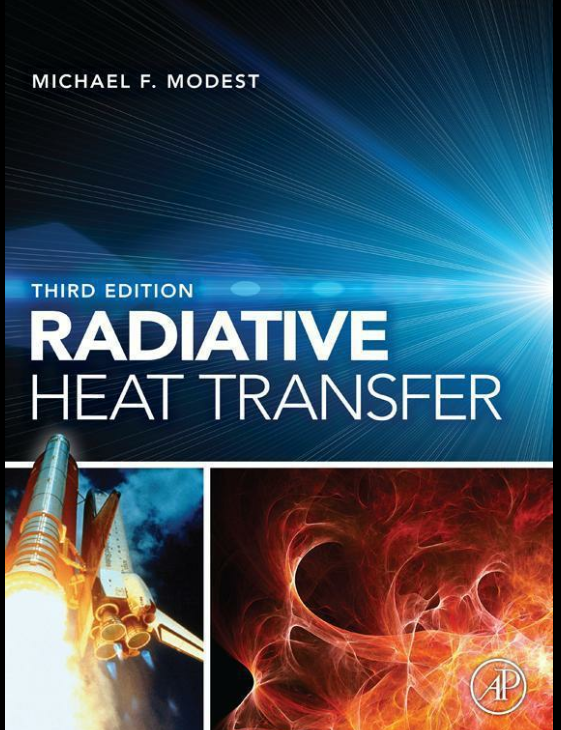
\includegraphics[width=3.11in,height=4.05in]{./media/image1.png}
	\end{Center}
\end{figure}


%%%%%%%%%%%%%%%%%%%% Figure/Image No: 1 Ends here %%%%%%%%%%%%%%%%%%%%

\par

\href{https://www.sciencedirect.com/book/9780123869449/radiative-heat-transfer}{https://www.sciencedirect.com/book/9780123869449/radiative-heat-transfer}\par

\section*{1 – Introduction}
\addcontentsline{toc}{section}{1 – Introduction}
The more advanced stuff$ \ldots $ \par


\vspace{\baselineskip}
What you should know:\par

\begin{itemize}
	\item Basic Conduction:  \( q^{''}=-k\triangledown T \) \par

	\item Basic Convection:  \( q^{''}=h \left( T-T_{\infty} \right)  \) \par

	\item Basic Radiation  \( q^{''}\propto \left( T^{4}-T_{\infty}^{4} \right)  \) \par


\vspace{\baselineskip}
Thermal radiation = electromagnetic wave\par


\vspace{\baselineskip}
Some recap on terms:\par

Refractive index  \( c_{n}=\frac{c_{0}}{n};c_{0}=2.998\ast10^{8}\frac{m}{s}~ \) \par



%%%%%%%%%%%%%%%%%%%% Figure/Image No: 2 starts here %%%%%%%%%%%%%%%%%%%%

\begin{figure}[H]
	\begin{Center}
		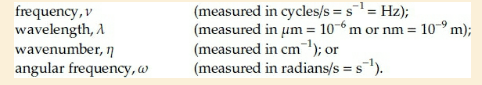
\includegraphics[width=5.02in,height=0.89in]{./media/image2.png}
	\end{Center}
\end{figure}


%%%%%%%%%%%%%%%%%%%% Figure/Image No: 2 Ends here %%%%%%%%%%%%%%%%%%%%

\par

 \[ c_{0}= \nu  \lambda   \left( for electromagnetic waves \right)  \] \par

 \[ c_{n}= \nu  \lambda _{n} \] \par

 \[  \epsilon =h \nu  \] \par

 \[  \nu =\frac{ \omega }{2 \pi }=\frac{c}{ \lambda }=c \eta  \] \par

 \[  \eta =\frac{1}{ \lambda }~ \left( wavenumber \right)  \] \par

Wavelength of thermal radiation:\par

 \[ 10^{-7}\text{m to }10^{2}m \] \par


\vspace{\baselineskip}

\end{itemize}\section*{What is a blackbody?}
\addcontentsline{toc}{section}{What is a blackbody?}


%%%%%%%%%%%%%%%%%%%% Figure/Image No: 3 starts here %%%%%%%%%%%%%%%%%%%%

\begin{figure}[H]
	\begin{Center}
		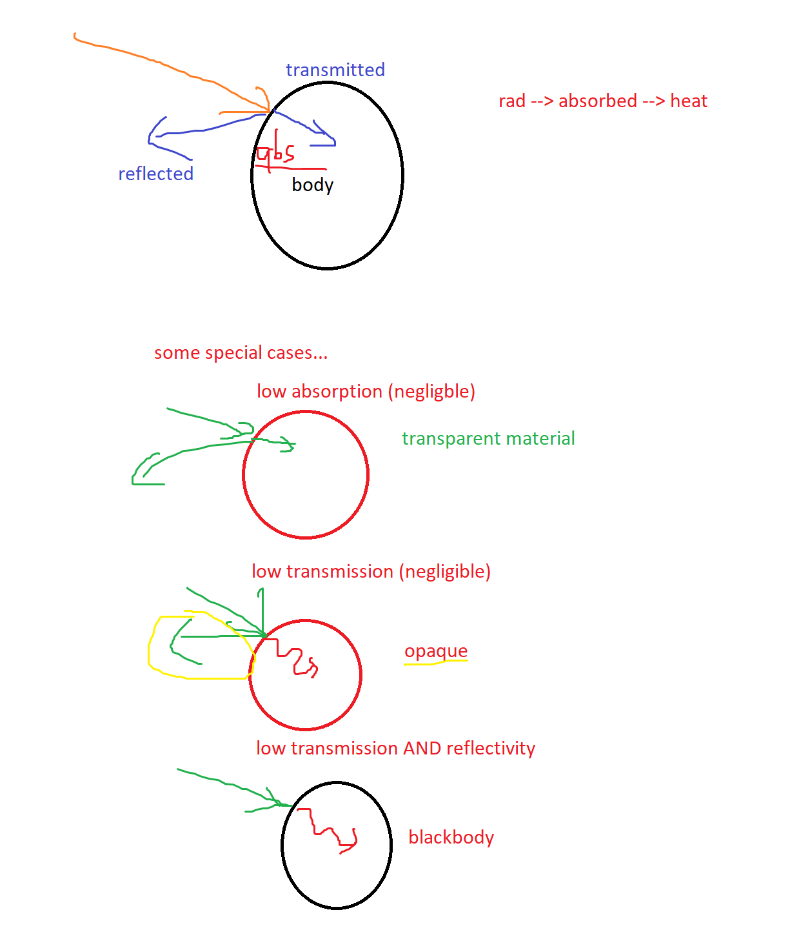
\includegraphics[width=3.58in,height=4.26in]{./media/image3.png}
	\end{Center}
\end{figure}


%%%%%%%%%%%%%%%%%%%% Figure/Image No: 3 Ends here %%%%%%%%%%%%%%%%%%%%

\par

We often say, that a blackbody is a good absorber, but absorbers are good emitters$ \ldots $ \par

How do we prove that?\par


\href{https://en.wikipedia.org/wiki/Kirchhoff\%27s_law_of_thermal_radiation}{https://en.wikipedia.org/wiki/Kirchhoff$'$s\_law\_of\_thermal\_radiation}\par


\setlength{\parskip}{0.0pt}
{\fontsize{10pt}{12.0pt}\selectfont \textcolor[HTML]{222222}{For an arbitrary body emitting and absorbing thermal radiation in thermodynamic equilibrium, the emissivity is equal to the absorptivity.}\par}\par


\vspace{\baselineskip}
 \[  \alpha = \varepsilon  in thermodynamic equilibrium, only radiation heat trf \] \par

\setlength{\parskip}{8.04pt}
\section*{Blackbody Emissions$ \ldots $ }
\addcontentsline{toc}{section}{Blackbody Emissions$ \ldots $ }
What exactly is absorptivity and emissivity?\par

Before we start, we need to look at emissive power$ \ldots $ \par



%%%%%%%%%%%%%%%%%%%% Figure/Image No: 4 starts here %%%%%%%%%%%%%%%%%%%%

\begin{figure}[H]
	\begin{Center}
		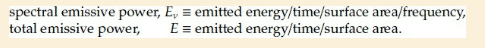
\includegraphics[width=5.05in,height=0.5in]{./media/image5.png}
	\end{Center}
\end{figure}


%%%%%%%%%%%%%%%%%%%% Figure/Image No: 4 Ends here %%%%%%%%%%%%%%%%%%%%

\par

How can we characterize the radiation coming off the body?\par

 \[ E_{ \nu }=\frac{energy}{time \cdot Area \cdot frequency} \] \par

For Total Emissive Power, Integrate across all frequency\par

 \[ E= \int _{0}^{\infty}E_{ \nu } d \nu  \] \par


\vspace{\baselineskip}
Special cases:\par

\begin{itemize}
	\item Blackbody\par

	\item Monochromatic (one frequency), eg. Laser\par

	\item Gray (energy is equally distributed across all frequencies)\par



%%%%%%%%%%%%%%%%%%%% Figure/Image No: 5 starts here %%%%%%%%%%%%%%%%%%%%

\begin{figure}[H]
	\begin{Center}
		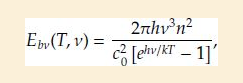
\includegraphics[width=2.53in,height=0.86in]{./media/image6.png}
	\end{Center}
\end{figure}


%%%%%%%%%%%%%%%%%%%% Figure/Image No: 5 Ends here %%%%%%%%%%%%%%%%%%%%

\par

 \[ E_{b \nu } \left( T, \nu  \right) =\frac{2 \pi h \nu ^{3}n^{2}}{c_{0}^{2} \left[ \exp  \left( \frac{h \nu }{kT} \right) -1 \right] } \] \par

Based on quantum physics$ \ldots $ \par



%%%%%%%%%%%%%%%%%%%% Figure/Image No: 6 starts here %%%%%%%%%%%%%%%%%%%%

\begin{figure}[H]
	\begin{Center}
		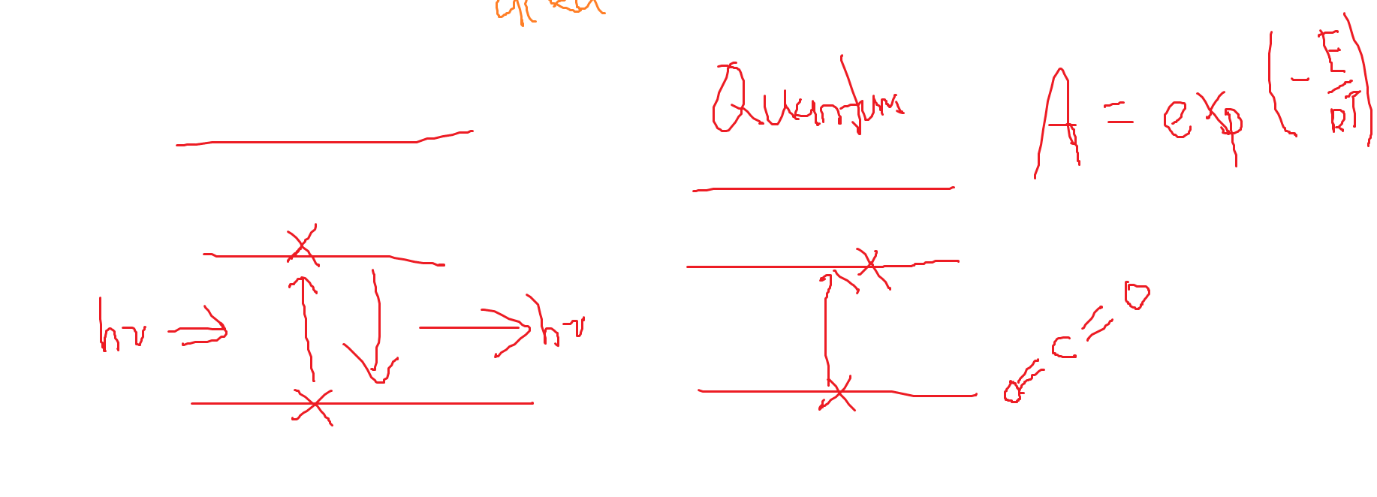
\includegraphics[width=6.27in,height=2.26in]{./media/image7.png}
	\end{Center}
\end{figure}


%%%%%%%%%%%%%%%%%%%% Figure/Image No: 6 Ends here %%%%%%%%%%%%%%%%%%%%

\par



 %%%%%%%%%%%%  Starting New Page here %%%%%%%%%%%%%%

\newpage

\vspace{\baselineskip}

%%%%%%%%%%%%%%%%%%%% Figure/Image No: 7 starts here %%%%%%%%%%%%%%%%%%%%

\begin{figure}[H]
	\begin{Center}
		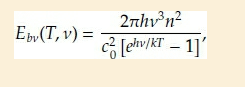
\includegraphics[width=2.55in,height=0.91in]{./media/image8.png}
	\end{Center}
\end{figure}


%%%%%%%%%%%%%%%%%%%% Figure/Image No: 7 Ends here %%%%%%%%%%%%%%%%%%%%

\par

Planck’s Law\par


\vspace{\baselineskip}
 \[ E_{b \nu } \left( T, \nu  \right) =\frac{2 \pi h \nu ^{3}n^{2}}{c_{0}^{2}~ \left[ \exp  \left( \frac{h \nu }{kT} \right) -1 \right] } \] \par

 \[ E_{b \nu } \left( T, \nu  \right) =\frac{2 \pi h \nu ^{3}}{c_{n}^{2}~ \left[ \exp  \left( \frac{h \nu }{kT} \right) -1 \right] } \] \par

\begin{enumerate}
	\item Blackbody emits radiation in all directions equally
\end{enumerate}\par

Total energy emitted?\par

 \[ E_{b} \left( T \right) =  \int _{0}^{\infty}\frac{2 \pi h \nu ^{3}n^{2}}{c_{0}^{2}~ \left[ \exp  \left( \frac{h \nu }{kT} \right) -1 \right] } d \nu  \] \par



%%%%%%%%%%%%%%%%%%%% Figure/Image No: 8 starts here %%%%%%%%%%%%%%%%%%%%

\begin{figure}[H]
	\begin{Center}
		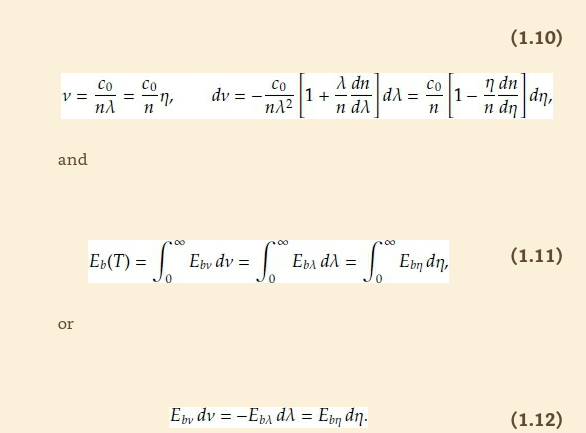
\includegraphics[width=6.1in,height=4.51in]{./media/image9.png}
	\end{Center}
\end{figure}


%%%%%%%%%%%%%%%%%%%% Figure/Image No: 8 Ends here %%%%%%%%%%%%%%%%%%%%

\par

 \[ E_{b} \left( T \right) = \int _{0}^{\infty}E_{b \nu } d \nu =  \int _{0}^{\infty}\frac{2 \pi h \nu ^{3}n^{2}}{c_{0}^{2}~ \left[ \exp  \left( \frac{h \nu }{kT} \right) -1 \right] } d \nu = \int _{0}^{\infty}E_{b \lambda }d \lambda  \] \par

 \[ E_{b} \left( T \right) = \int _{0}^{\infty}E_{b \nu } d \nu =  \int _{0}^{\infty}E_{b \lambda }d \lambda  \] \par

 \[ d \nu = \left( -\frac{c_{0}}{n \lambda } \right)  \left[ 1+\frac{ \lambda }{n}\frac{dn}{d \lambda } \right] d \lambda  \] \par

 \[ E_{b} \left( T \right) =  \int _{\infty}^{0}\frac{2 \pi h \nu ^{3}n^{2}}{c_{0}^{2}~ \left[ \exp  \left( \frac{h \nu }{kT} \right) -1 \right] }~ \left( -\frac{c_{0}}{n \lambda } \right)  \left[ 1+\frac{ \lambda }{n}\frac{dn}{d \lambda } \right] d \lambda  \] \par

 \[ E_{b} \left( T \right) =  \int _{0}^{\infty}\frac{2 \pi h \nu ^{3}n^{2}}{c_{0}^{2}~ \left[ \exp  \left( \frac{h \nu }{kT} \right) -1 \right] }~ \left( \frac{c_{0}}{n \lambda } \right)  \left[ 1+\frac{ \lambda }{n}\frac{dn}{d \lambda } \right] d \lambda =  \int _{0}^{\infty}E_{b \lambda }d \lambda  \] \par


\vspace{\baselineskip}
 \[ E_{b \lambda }=\frac{2 \pi h \nu ^{3}n^{2}}{c_{0}^{2}~ \left[ \exp  \left( \frac{h \nu }{kT} \right) -1 \right] }~ \left( \frac{c_{0}}{n \lambda } \right)  \left[ 1+\frac{ \lambda }{n}\frac{dn}{d \lambda } \right]  \] \par

 \[  \nu =\frac{c_{0}}{n \lambda } \] \par

 \[ E_{b \lambda }=\frac{2 \pi h \left( \frac{c_{0}}{n \lambda } \right) ^{3}n^{2}}{c_{0}^{2}~ \left[ \exp  \left( \frac{h \left( \frac{c_{0}}{n \lambda } \right) }{kT} \right) -1 \right] }~ \left( \frac{c_{0}}{n \lambda } \right)  \left[ 1+\frac{ \lambda }{n}\frac{dn}{d \lambda } \right]  \] \par

 \[ E_{b} \left( T \right) = \int _{0}^{\infty}E_{b \nu } d \nu =  \int _{0}^{\infty}E_{b \eta }d \eta  \] \par

 \[ E_{b} \left( T \right) = \int _{0}^{\infty}\frac{2 \pi h \nu ^{3}n^{2}}{c_{0}^{2}~ \left[ \exp  \left( \frac{h \nu }{kT} \right) -1 \right] } d \nu  \] \par

 \[ d \nu =\frac{c_{0}}{n} \left[ 1-\frac{ \eta }{n} \left( \frac{dn}{d \eta } \right)  \right] d \eta  \] \par


\vspace{\baselineskip}
 \[ E_{b} \left( T \right) =  \int _{0}^{\infty}\frac{2 \pi h \nu ^{3}n^{2}}{c_{0}^{2}~ \left[ \exp  \left( \frac{h \nu }{kT} \right) -1 \right] }\frac{c_{0}}{n} \left[ 1-\frac{ \eta }{n} \left( \frac{dn}{d \eta } \right)  \right] d \eta  \] \par

 \[  \nu =\frac{c_{0}}{n} \eta  \] \par

 \[ E_{b} \left( T \right) =  \int _{0}^{\infty}\frac{2 \pi h \left( \frac{c_{0}}{n} \eta  \right) ^{3}n^{2}}{c_{0}^{2}~ \left[ \exp  \left( \frac{h \left( \frac{c_{0}}{n} \eta  \right) }{kT} \right) -1 \right] }\frac{c_{0}}{n} \left[ 1-\frac{ \eta }{n} \left( \frac{dn}{d \eta } \right)  \right] d \eta  \] \par

 \[ E_{b \eta }=\frac{2 \pi h \left( \frac{c_{0}}{n} \eta  \right) ^{3}n^{2}}{c_{0}^{2}~ \left[ \exp  \left( \frac{h \left( \frac{c_{0}}{n} \eta  \right) }{kT} \right) -1 \right] }\frac{c_{0}}{n} \left[ 1-\frac{ \eta }{n} \left( \frac{dn}{d \eta } \right)  \right]  \] \par

\uline{If we have constant refractive index (not always the case, but true for vacuum and gases)}\par

 \[ E_{b \eta }=\frac{2 \pi h \left( \frac{c_{0}}{n} \eta  \right) ^{3}n^{2}}{c_{0}^{2}~ \left[ \exp  \left( \frac{h \left( \frac{c_{0}}{n} \eta  \right) }{kT} \right) -1 \right] }\frac{c_{0}}{n} \] \par

 \[ E_{b \lambda }=\frac{2 \pi h \left( \frac{c_{0}}{n \lambda } \right) ^{3}n^{2}}{c_{0}^{2}~ \left[ \exp  \left( \frac{h \left( \frac{c_{0}}{n \lambda } \right) }{kT} \right) -1 \right] }~ \left( \frac{c_{0}}{n \lambda } \right)  \] \par

What is the wavelength/frequency/wavenumber where most energy is emitted?\par

At a fixed temperature T, what is the frequency?\par

 \[ E_{b \nu } \left( T, \nu  \right) =\frac{2 \pi h \nu ^{3}}{c_{n}~ \left[ \exp  \left( \frac{h \nu }{kT} \right) -1 \right] } \] \par

 \[ \frac{ \partial }{ \partial  \nu }E_{b \nu } \left( T, \nu  \right) =0 \] \par

 \[ \frac{ \partial }{ \partial  \nu }\frac{2 \pi h \nu ^{3}}{c_{n}~ \left[ \exp  \left( \frac{h \nu }{kT} \right) -1 \right] }=0 \] \par

 \[ \frac{ \partial }{ \partial  \nu }\frac{ \nu ^{3}}{c_{n}~ \left[ \exp  \left( \frac{h \nu }{kT} \right) -1 \right] }=0 \] \par

 \[ \frac{ \partial }{ \partial  \lambda } \] \par



%%%%%%%%%%%%%%%%%%%% Figure/Image No: 9 starts here %%%%%%%%%%%%%%%%%%%%

\begin{figure}[H]
	\begin{Center}
		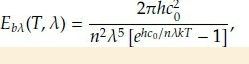
\includegraphics[width=2.59in,height=0.67in]{./media/image10.png}
	\end{Center}
\end{figure}


%%%%%%%%%%%%%%%%%%%% Figure/Image No: 9 Ends here %%%%%%%%%%%%%%%%%%%%

\par

 \[ E_{b \lambda } \left( T, \lambda  \right) =\frac{2 \pi hc_{0}^{2}}{n^{2} \lambda ^{5} \left[ \exp  \left( \frac{h \left( \frac{c_{0}}{n \lambda } \right) }{kT} \right) -1 \right] } \] \par



%%%%%%%%%%%%%%%%%%%% Figure/Image No: 10 starts here %%%%%%%%%%%%%%%%%%%%

\begin{figure}[H]
	\begin{Center}
		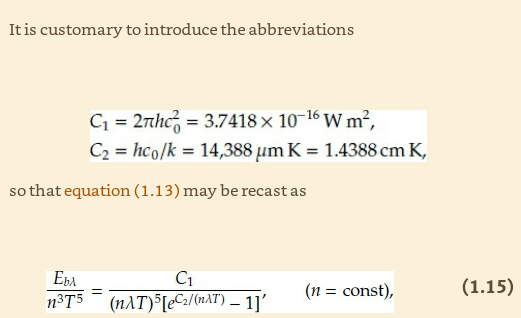
\includegraphics[width=5.43in,height=3.31in]{./media/image11.png}
	\end{Center}
\end{figure}


%%%%%%%%%%%%%%%%%%%% Figure/Image No: 10 Ends here %%%%%%%%%%%%%%%%%%%%

\par

 \[ \frac{E_{b \lambda } \left( T, \lambda  \right) }{n^{3}T^{5}}=\frac{2 \pi hc_{0}^{2}}{T^{5}n^{5} \lambda ^{5} \left[ \exp  \left( \frac{h \left( \frac{c_{0}}{n \lambda } \right) }{kT} \right) -1 \right] } \] \par

We do this so we can group the terms\par

 \( n \lambda T  \) together\par

 \[ \frac{E_{b \lambda } \left( T, \lambda  \right) }{n^{3}T^{5}}=\frac{2 \pi hc_{0}^{2}}{ \left( n \lambda T \right) ^{5} \left[ \exp  \left( \frac{hc_{0}}{k \left( n \lambda T \right) } \right) -1 \right] } \] \par


\vspace{\baselineskip}
 \[ \frac{ \partial }{ \partial  \left( n \lambda T \right) }~\frac{E_{b \lambda } \left( T, \lambda  \right) }{n^{3}T^{5}}=\frac{ \partial }{ \partial  \left( n \lambda T \right) }\frac{2 \pi hc_{0}^{2}}{ \left( n \lambda T \right) ^{5} \left[ \exp  \left( \frac{hc_{0}}{k \left( n \lambda T \right) } \right) -1 \right] }=0 \] \par

 \[ \frac{ \partial }{ \partial  \left( n \lambda T \right) }\frac{2 \pi hc_{0}^{2}}{ \left( n \lambda T \right) ^{5} \left[ \exp  \left( \frac{hc_{0}}{k \left( n \lambda T \right) } \right) -1 \right] }=0 \] \par

When we set the derivative to 0, we find the maximum  \( \frac{E_{b \lambda } \left( T, \lambda  \right) }{n^{3}T^{5}} \) , which corresponds to the maximum energy emitted for a particular wavelength.\par



%%%%%%%%%%%%%%%%%%%% Figure/Image No: 11 starts here %%%%%%%%%%%%%%%%%%%%

\begin{figure}[H]
	\begin{Center}
		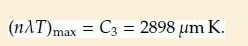
\includegraphics[width=2.58in,height=0.48in]{./media/image12.png}
	\end{Center}
\end{figure}


%%%%%%%%%%%%%%%%%%%% Figure/Image No: 11 Ends here %%%%%%%%%%%%%%%%%%%%

  holds constant for all black bodies\par

\href{https://en.wikipedia.org/wiki/Wien's_displacement_law}{https://en.wikipedia.org/wiki/Wien's\_displacement\_law}\par

So, Planck’s law describes \textbf{black body emission}, Wien’s displacement law describes the wavelength for which maximum energy is emitted in the Planck spectrum. \par


\vspace{\baselineskip}

\end{itemize}\section*{Solid Angles and Directional Dependence}
\addcontentsline{toc}{section}{Solid Angles and Directional Dependence}
\par

Direction is  \( \hat{s} \) \par

The normal area projected in the direction  \( \hat{s} \)  is  \( dA_{j}^{''} \rightarrow normal area receiving the radiation \) \par

 \[ dA \rightarrow area emitting the radiation \] \par

 \[ dA_{j}^{''}=dA_{j}\cos  \theta _{j} \] \par

Solid angle?\par

 \[ solid angle=\frac{dA_{j}^{''}}{r^{2}}=\frac{dA_{j}\cos  \theta _{j}}{r^{2}} \] \par

 \[ d \Omega =\frac{dA_{j}\cos  \theta _{j}}{r^{2}}=\frac{ \left( r sin \theta  d \psi  \right) \ast \left( r d \theta  \right) }{r^{2}}=\sin  \theta d \theta  d \psi  \] \par

 \[ I \left( T, \theta , \psi , \nu  \right) =I \left( T, \Omega , \nu  \right)  \] \par

\par

\par

Just note the difference between spectral intensity and total intensity. \par

 \[ E= \int _{d \Omega }^{}d \Omega  I \left( r,\overrightarrow{s} \right)  \] \par

 \[ E_{ \nu }= \int _{d \Omega }^{}d \Omega I \left( r,\overrightarrow{s}, \nu  \right)  \] \par

\par

Spectral intensity: per unit \textbf{Normal area}\par

Spectral emissive power: per unit \textbf{surface area}\par

 \[ E \left( r, \theta , \psi  \right)  dA=I \left( r, \theta , \psi  \right) ~dA_{p} \] \par

 \[ dA_{p}=dA\cos  \theta  \] \par

 \[ E \left( r, \theta , \psi  \right)  =I \left( r, \theta , \psi  \right) \cos  \theta  \] \par

(Lambert’s law)\par

Unit of solid angle: \uline{steradians}.\par

 \[  \Omega _{hemisphere}=\frac{A}{r^{2}}=\frac{\frac{4 \pi r^{2}}{2}}{r^{2}}=2 \pi  steradians  \] \par

\section*{Emissivity and absorptivity}
\addcontentsline{toc}{section}{Emissivity and absorptivity}
By definition:\par

Emissivity: energy emitted by a real surface compared to a blackbody\par

Absorptivity: energy absorbed by a real surface compared to a blackbody\par

\par

Spectral emissivity\par

 \[  \epsilon  \left( T, \theta , \psi , \nu  \right) =\frac{E_{ \nu } \left( T, \theta , \psi , \nu  \right) }{E_{ \nu b} \left( T, \theta , \psi , \nu  \right) }=\frac{I_{ \nu } \left( T, \theta , \psi , \nu  \right) \cos  \theta }{I_{ \nu b} \left( T, \theta , \psi , \nu  \right) \cos  \theta }=\frac{I_{ \nu } \left( T, \theta , \psi , \nu  \right) }{I_{ \nu b} \left( T, \theta , \psi , \nu  \right) } \] \par

Spectral absorptivity\par

 \[  \alpha  \left( T, \theta , \psi , \nu  \right) =\frac{E_{ \nu ABS} \left( T, \theta , \psi , \nu  \right) }{E_{ \nu bABS} \left( T, \theta , \psi , \nu  \right) }=\frac{I_{ \nu ABS} \left( T, \theta , \psi , \nu  \right) \cos  \theta }{I_{ \nu bABS} \left( T, \theta , \psi , \nu  \right) \cos  \theta }=\frac{I_{ \nu ABS} \left( T, \theta , \psi , \nu  \right) }{I_{ \nu bABS } \left( T, \theta , \psi , \nu  \right) } \] \par


\vspace{\baselineskip}

\vspace{\baselineskip}
\section*{Radiative Heat Transfer Between Surfaces}
\addcontentsline{toc}{section}{Radiative Heat Transfer Between Surfaces}
Case 1: black surfaces\par

\par

Case 2: non black surfaces\par

\par

Case 2.1: grey surfaces\par

\par

Case 2.2 grey diffuse surfaces\par

\par

The simplest case\par

Between two black surfaces$ \ldots $ \par

\par

 \[ I_{b \lambda }=\frac{2 \pi hc_{0}^{2}}{n^{2} \lambda ^{5} \left[ \exp  \left( \frac{h \left( \frac{c_{0}}{n \lambda } \right) }{kT} \right) -1 \right] }\frac{1}{\cos  \theta } \] \par

 \[ E \left( r, \theta , \psi  \right)  =I \left( r, \theta , \psi  \right) \cos  \theta  \] \par

In total, since spectrum is not important, we use:\par

\par

\par

 \[ E_{b \lambda }=\frac{2 \pi hc_{0}^{2}}{n^{2} \lambda ^{5} \left[ \exp  \left( \frac{h \left( \frac{c_{0}}{n \lambda } \right) }{kT} \right) -1 \right] } \] \par

 \[ I_{b}=n^{2} \sigma T^{4}~\frac{1}{\cos  \theta }~ \left( \text{power per unit solid angle per unit normal area} \right)  \] \par

We want to consider the geometric effects on radiation heat transfer$ \ldots $ \par

\uline{We need to consider, view factors.  next video}\par

\par

Principle: So we need to, in general, integrate the heat transfer between the infinitesimally small areas until we get full heat transfer say between A1 and A2$ \ldots $ \par

\begin{enumerate}
	\item How do we find heat transfer between dA1 and dA2?
\end{enumerate}\par

 \[ I_{b \lambda }=\frac{power}{solid angle~\ast~normal~area~\ast~wavelength} \] \par

 \[ I_{b}= \int _{0}^{\infty}I_{b \lambda }d \lambda =\frac{power}{solid~angle\ast~normal~area} \] \par

Heat transfer\par

 \[ dq_{12}=I_{b}\ast \left( \text{normal area} \right) \ast \left( solid angle \right)  \] \par

Normal area of dA2 is  \( dA_{2}\cos  \theta _{2} \) \par

Normal area of dA1 is  \( dA_{1}\cos  \theta _{1} \) \par

 \[ dq_{12}=I_{b}\ast \left( dA_{1}\cos  \theta _{1} \right) \ast \left( solid angle \right)  \] \par

 \[ solid angle=\frac{dA_{normal}}{r^{2}} \] \par

 \[ dq_{12}=I_{b}\ast \left( dA_{1}\cos  \theta _{1} \right) \ast \left( \frac{dA_{normal}}{r^{2}} \right)  \] \par

 \[ dq_{12}=I_{b}\ast \left( dA_{1}\cos  \theta _{1} \right) \ast \left( \frac{dA_{2}\cos  \theta _{2}}{r^{2}} \right)  \] \par

 \[ q_{12}= \int _{A_{1}}^{} \int _{A_{2}}^{}~I_{b}\ast \left( \cos  \theta _{1} \right) \ast \left( \frac{\cos  \theta _{2}}{r^{2}} \right) dA_{2}dA_{1} \] \par

\textbf{How to find  \( I_{b} \) }\par

\par

Total energy output?\par

 \[ \frac{power}{area}~\ast~area=n^{2} \sigma T^{4}~\ast~dA_{3}=E_{b} \left( T \right) ~\ast~dA_{3} \] \par

Express total energy output in terms of intensity?\par

 \[ I_{b} \left( T \right) =\frac{power}{normal area~\ast~solid angle} \] \par

 \[ power=I_{b} \left( T \right) ~\ast~normal area~\ast~solid angle \] \par

 \[ power= \int _{ \Omega }^{}I_{b} \left( T \right) ~\ast~dA_{3}\cos  \theta _{3}~\ast~\frac{dA_{4}\cos  \theta _{4}}{r^{2}} \] \par

 \[ d \Omega =\frac{dA_{4}\cos  \theta _{4}}{r^{2}}=\sin  \theta _{3}~d \theta _{3}~d \psi _{3} \] \par

 \[ power= \int _{0}^{2 \pi } \int _{0}^{\frac{ \pi }{2}}I_{b} \left( T \right) \ast~dA_{3}\cos  \theta _{3}\ast\sin  \theta _{3}~d \theta _{3}~d \psi _{3} \] \par

 \[ E_{b} \left( T \right) \ast~dA_{3}= \int _{0}^{2 \pi } \int _{0}^{\frac{ \pi }{2}}I_{b} \left( T \right) \ast~dA_{3}\cos  \theta _{3}\ast\sin  \theta _{3}~d \theta _{3}~d \psi _{3} \] \par

 \[ E_{b} \left( T \right) = \int _{0}^{2 \pi } \int _{0}^{\frac{ \pi }{2}}I_{b} \left( T \right) \cos  \theta _{3}\sin  \theta _{3}~d \theta _{3}~d \psi _{3} \] \par

According to Kirchhoff’s law, blackbody intensity is direction independent$ \ldots $ \par

 \[ E_{b} \left( T \right) =I_{b} \left( T \right)  \int _{0}^{2 \pi } \int _{0}^{\frac{ \pi }{2}}\cos  \theta _{3}\sin  \theta _{3}~d \theta _{3}~d \psi _{3} \] \par

 \[ E_{b} \left( T \right) =I_{b} \left( T \right)  2 \pi  \int _{0}^{\frac{ \pi }{2}}\cos  \theta _{3}\sin  \theta _{3}~d \theta _{3} \] \par

 \[ E_{b} \left( T \right) =I_{b} \left( T \right)  2 \pi  \left( \frac{1}{2} \right)  \] \par

 \[ E_{b} \left( T \right) =I_{b} \left( T \right)   \pi  \] \par

 \[ I_{b} \left( T \right) =\frac{E_{b} \left( T \right) }{ \pi }=\frac{n^{2} \sigma T^{4}}{ \pi } \] \par

But there could be some confusion, what is this???\par

 \[ E \left( r, \theta , \psi  \right)  =I \left( r, \theta , \psi  \right) \cos  \theta  \] \par

 \[ E \left( r, \theta , \psi  \right) =\frac{power}{area\ast~solid angle} \] \par

 \[ E_{b} \left( T \right) =\frac{power}{area} \] \par

 \[ E \left( r, \theta , \psi  \right) =\frac{power}{area\ast~solid angle} \] \par

 \[ I \left( r, \theta , \psi  \right) =\frac{power}{normal area\ast~solid angle} \] \par

 \[ \frac{power}{\text{solid angle}}=E \left( r, \theta , \psi  \right) ~dA_{3}=I \left( r, \theta , \psi  \right) ~dA_{3}\cos  \theta _{3} \] \par

 \[ E \left( r, \theta , \psi  \right) =I \left( r, \theta , \psi  \right) ~\cos  \theta _{3} \] \par

 \[ E \left( r, \theta , \psi  \right)  \rightarrow takes into account solid angle \] \par

 \( E_{b} \left( T \right)  \)  doesn’t take into account solid angle\par

Substitute back into our heat transfer expression:\par

 \[ q_{12}= \int _{A_{1}}^{} \int _{A_{2}}^{}~I_{b} \left( T \right) \ast \left( \cos  \theta _{1} \right) \ast \left( \frac{\cos  \theta _{2}}{r^{2}} \right) dA_{2}dA_{1} \] \par

 \[ I_{b} \left( T \right) =\frac{n^{2} \sigma T^{4}}{ \pi } \] \par

 \[ q_{12}= \int _{A_{1}}^{} \int _{A_{2}}^{}~\frac{n^{2} \sigma T_{1}^{4}}{ \pi }\ast \left( \cos  \theta _{1} \right) \ast \left( \frac{\cos  \theta _{2}}{r^{2}} \right) dA_{2}dA_{1} \] \par

 \[  \left( \frac{\cos  \theta _{2}}{r^{2}} \right) dA_{2}=d \Omega =\sin  \theta _{2}~d \theta _{2}~d \psi _{2} \] \par

Let’s say you wanted to account for the shape factor or view factor of the heat transfer$ \ldots $ \par

\par

We account for the shape using this thing called view factors.\par

\par


\vspace{\baselineskip}
\textbf{Diffuse} view factor, configuration factor, shape factor or angle factor\par

\par

Diffuse assumption$ \ldots $ \par

Applies to:\par
\begin{itemize}
	\item Blackbodies\par

	\item Diffuse surfaces\par


	\item Gray or otherwise\par
\end{itemize}


\vspace{\baselineskip}
 \[ q_{12}= \int _{A_{1}}^{} \int _{A_{2}}^{}~\frac{n^{2} \sigma T_{1}^{4}}{ \pi }\ast \left( \cos  \theta _{1} \right) \ast \left( \frac{\cos  \theta _{2}}{r^{2}} \right) dA_{2}dA_{1} \] \par

 \[ \text{view facto}r_{1-2}=\frac{q_{12}}{\text{total heat transfer from 1 }}=\frac{ \int _{A_{1}}^{} \int _{A_{2}}^{}~\frac{n^{2} \sigma T_{1}^{4}}{ \pi }\ast \left( \cos  \theta _{1} \right) \ast \left( \frac{\cos  \theta _{2}}{r^{2}} \right) dA_{2}dA_{1}}{E_{b} \left( T \right) \ast~A_{1}} \] \par

 \[ \text{view facto}r_{1-2}=\frac{q_{12}}{\text{total heat transfer from 1 }}=\frac{ \int _{A_{1}}^{} \int _{A_{2}}^{}~\frac{n^{2} \sigma T_{1}^{4}}{ \pi }\ast \left( \cos  \theta _{1} \right) \ast \left( \frac{\cos  \theta _{2}}{r^{2}} \right) dA_{2}dA_{1}}{n^{2} \sigma T_{1}^{4}\ast~A_{1}} \] \par

If we have constant T1 across the board,\par

 \[ \text{view facto}r_{1-2}=\frac{q_{12}}{\text{total heat transfer from 1 }}=\frac{ \int _{A_{1}}^{} \int _{A_{2}}^{}~\frac{1}{ \pi }\ast \left( \cos  \theta _{1} \right) \ast \left( \frac{\cos  \theta _{2}}{r^{2}} \right) dA_{2}dA_{1}}{A_{1}} \] \par

 \[ F_{1-2}=\frac{1}{A_{1}} \int _{A_{1}}^{} \int _{A_{2}}^{}~ \left( \cos  \theta _{1} \right) \ast \left( \frac{\cos  \theta _{2}}{ \pi r^{2}} \right) dA_{2}dA_{1} \] \par

\par

\par

 \[ F_{1-2}=\frac{1}{A_{1}} \int _{A_{1}}^{} \int _{A_{2}}^{}~ \left( \cos  \theta _{1} \right) \ast \left( \frac{\cos  \theta _{2}}{ \pi S^{2}} \right) dA_{2}dA_{1} \] \par

Let’s say we want view factor from dA1 to dA2\par

 \[ dq_{12}=I_{b}\ast \left( dA_{1}\cos  \theta _{1} \right) \ast \left( \frac{dA_{2}\cos  \theta _{2}}{S^{2}} \right)  \] \par

 \[ I_{b}=\frac{E_{b} \left( T \right) }{ \pi } \] \par

Total energy leaving dA1 =  \( E_{b} \left( T \right) ~dA_{1} \) \par

 \[ F_{dA_{1}-dA_{2}}=\frac{\frac{E_{b} \left( T \right) }{ \pi } \left( dA_{1}\cos  \theta _{1} \right)  \left( \frac{dA_{2}\cos  \theta _{2}}{S^{2}} \right) }{E_{b} \left( T \right) ~dA_{1}} \] \par

 \[ F_{dA_{1}-dA_{2}}= \left( \cos  \theta _{1} \right)  \left( \frac{dA_{2}\cos  \theta _{2}}{ \pi S^{2}} \right)  \] \par

Just for exercise, dA1 to A2\par

 \[ q_{dA_{1}-dA_{2}}= \int _{A_{2}}^{}I_{b}\ast \left( dA_{1}\cos  \theta _{1} \right) \ast \left( \frac{dA_{2}\cos  \theta _{2}}{S^{2}} \right)  \] \par

 \[ F_{dA_{1}-A_{2}}=\frac{ \int _{A_{2}}^{}I_{b}\ast \left( dA_{1}\cos  \theta _{1} \right) \ast \left( \frac{dA_{2}\cos  \theta _{2}}{S^{2}} \right) }{E_{b} \left( T \right) ~dA_{1}} \] \par

 \[ F_{dA_{1}-A_{2}}= \int _{A_{2}}^{} \left( \cos  \theta _{1} \right)  \left( \frac{dA_{2}\cos  \theta _{2}}{ \pi S^{2}} \right)  \] \par

\par

Just for the other exercise A1 to dA2\par

 \[ q_{dA_{1}-dA_{2}}= \int _{A_{1}}^{}I_{b}\ast \left( dA_{1}\cos  \theta _{1} \right) \ast \left( \frac{dA_{2}\cos  \theta _{2}}{S^{2}} \right)  \] \par

 \[ F_{A_{1}-dA_{2}}=\frac{ \int _{A_{1}}^{}\frac{E_{b} \left( T \right) }{ \pi }\ast \left( dA_{1}\cos  \theta _{1} \right) \ast \left( \frac{dA_{2}\cos  \theta _{2}}{S^{2}} \right) }{E_{b} \left( T \right) A_{1}} \] \par

 \[ F_{A_{1}-dA_{2}}=\frac{ \int _{A_{1}}^{} \left( dA_{1}\cos  \theta _{1} \right)  \left( \frac{dA_{2}\cos  \theta _{2}}{ \pi S^{2}} \right) }{A_{1}} \] \par

After view factors$ \ldots $ \par

\uline{What then is the application or relevance?}\par

We want to study heat trf between real surfaces$ \ldots $ \par

\par

 \[ F_{12}=\frac{q_{1-2}}{E_{b} \left( T \right) A_{1}} \] \par

 \[ q_{1-2}= \left( E_{b} \left( T \right) A_{1} \right) ~F_{12} \] \par

So what is more representative of a real system?\par

\begin{itemize}
	\item Maybe surfaces are gray (but diffuse)\par

	\item Maybe there is incoming radiation from outside$ \ldots $ \par

	\item There is heat radiation from outside, and heat transfer from A2 to A1\par

	\item Conduction and convection (later on)\par

	\item There can be a participating medium (air or such)\par
\end{itemize}



\vspace{\baselineskip}
For now we want to, based on heat trf from A1 to A2, A2 to A1 and heat trf from external source, develop an energy balance to determine \uline{net heat transfer from A1}\par


\vspace{\baselineskip}
\par

\par

\par

 \[ q \left( r \right) ~dA_{1}=E_{b} \left( T_{1},r \right) ~dA_{1}-H_{0} \left( r \right) ~dA_{1}- \int _{A_{2}}^{}E_{b} \left( T_{2},r^{'} \right) ~dF_{dA_{2}-dA_{1}}~dA_{2}~ \] \par

 \[ q \left( r \right)  =E_{b} \left( T_{1},r \right) -H_{0} \left( r \right)  - \int _{A_{2}}^{}E_{b} \left( T_{2},r^{'} \right) ~dF_{dA_{2}-dA_{1}}\frac{dA_{2}}{dA_{1}}~ \] \par

Reciprocity relation\par

 \[ dA_{1}~dF_{dA_{1}-dA_{2}}=dA_{2}~dF_{dA_{2}-dA_{1}}~ \] \par

 \[ dF_{dA_{1}-dA_{2}}=dF_{dA_{2}-dA_{1}}\frac{dA_{2}}{dA_{1}} \] \par

Substituting back, we get,\par

 \[ q \left( r \right)  =E_{b} \left( T_{1},r \right) -H_{0} \left( r \right)  - \int _{A_{2}}^{}E_{b} \left( T_{2},r^{'} \right) ~dF_{dA_{1}-dA_{2}}~ \] \par

The view factor is as such:\par

\par

\par

 \[ q \left( r \right)  =E_{b} \left( T_{1},r \right) -H_{0} \left( r \right)  - \int _{A_{2}}^{}E_{b} \left( T_{2},r^{'} \right) \frac{\cos  \theta _{1}\cos  \theta _{2}}{ \pi S^{2}}~dA_{2}~ \] \par

One simple example of heat trf between black surfaces, before we go onto more complicated heat trf to gray surfaces$ \ldots $ \par

Eg 5.1 in Michael F Modest Textbook.\par

\par

What is the net heat transfer rate from each surface?\par

\par

 \[ q \left( r \right)  =E_{b} \left( T_{1},r \right) -H_{0} \left( r \right)  - \int _{A_{2}}^{}E_{b} \left( T_{2},r^{'} \right) \frac{\cos  \theta _{1}\cos  \theta _{2}}{ \pi S^{2}}~dA_{2}~ \] \par

\par

\par

 \[ q_{1}=F_{1-2} \left( E_{b1}-E_{b2} \right) +F_{1-3} \left( E_{b1}-E_{b3} \right) +F_{1-4} \left( E_{b1}-E_{b4} \right)  \] \par

 \[ q_{1}=F_{1-2} \left( E_{b1}-E_{b2} \right) +F_{1-4} \left( E_{b1}-E_{b4} \right)  \] \par

 \( F_{1-2}=F_{1-4} \)   symmetry\par

 \[ E_{b4}=E_{b2}  \left( same temp \right)  \] \par

 \[ q_{1}=2F_{1-2} \left( E_{b1}-E_{b2} \right) =q_{3} \] \par

\par

Calculation of view factors\par

\par

 \[ E_{b}=n^{2} \sigma T^{4} \] \par

\par

Derive expressions for heat transfer between gray surfaces (diffuse)\par

\par

Recap on gray surfaces\par

\par

\par

Energy balance across dA\textsubscript{1}\par

 \[  \varepsilon =\frac{\text{heat emitted by surface}}{\text{heat emitted by }black~surface} \] \par

For \uline{diffuse} gray surface (what surfaces are diffuse)\par

\par

 \[ q_{net}~dA_{1}= \varepsilon  E_{b} \left( T \right) ~dA_{1}+ \rho H \left( r \right) ~dA_{1}-H \left( r \right) ~dA_{1} \] \par

 \[  \rho H \left( r \right) ~dA_{1}-H \left( r \right) ~dA_{1}=- \left( 1- \rho  \right) H \left( r \right) ~dA_{1}=- \alpha  H \left( r \right) ~dA_{1} \] \par

 \[  \alpha + \rho =1 \] \par

 \[ q_{net}~dA_{1}= \varepsilon  E_{b} \left( T \right) ~dA_{1}+ \rho H \left( r \right) ~dA_{1}-H \left( r \right) ~dA_{1} \] \par

 \[  \varepsilon  E_{b} \left( T \right) ~dA_{1}+ \rho H \left( r \right) ~dA_{1}=J \left( r \right) ~dA_{1} \] \par

\textbf{Radiosity  \( J \left( r \right)  \) }\par

This is the combined emitted and reflected radiation coming off a surface.\par

For a black surface, it is a special case of  \( J \left( r \right) =E_{b} \left( T \right)  \) \par

 \[ q_{net}~dA_{1}= \varepsilon  E_{b} \left( T \right) ~dA_{1}+ \rho H \left( r \right) ~dA_{1}-H \left( r \right) ~dA_{1} \] \par

Replace with radiosity\par

 \[ q_{net}~dA_{1}=J \left( r \right) ~dA_{1}-H \left( r \right) ~dA_{1} \] \par

Next question is what is H(r) for gray surface?\par

\par

 \[ H \left( r \right) ~dA_{1}=H_{0} \left( r \right) ~dA_{1}+ \int _{A_{2}}^{}J_{2} \left( r' \right) ~dA_{2}~dF_{dA_{2}-dA_{1}}~ \] \par

 \[ H \left( r \right)  =H_{0} \left( r \right)  + \int _{A_{2}}^{}J_{2} \left( r' \right) ~dA_{2}\frac{dF_{dA_{2}-dA_{1}}}{dA_{1}}~ \] \par

 \[ H \left( r \right)  =H_{0} \left( r \right)  + \int _{A_{2}}^{}J_{2} \left( r' \right) ~dF_{dA_{1}-dA_{2}}~ \] \par

 \[ q_{net}~dA_{1}=J \left( r \right) ~dA_{1}- \left( H_{0} \left( r \right)  + \int _{A_{2}}^{}J_{2} \left( r' \right) ~dF_{dA_{1}-dA_{2}} \right) ~dA_{1} \] \par

 \[ q_{net} =J_{1} \left( r \right)  - \left( H_{0} \left( r \right)  + \int _{A_{2}}^{}J_{2} \left( r' \right) ~dF_{dA_{1}-dA_{2}} \right)  \] \par

 \[ q_{net} =J_{1} \left( r \right)  -H_{0} \left( r \right) - \int _{A_{2}}^{}J_{2} \left( r' \right) ~dF_{dA_{1}-dA_{2}} \] \par

We have a bit of trouble still$ \ldots $ \par

We might know  \( E_{b} \left( T \right)  \)  and that will give us, the intensity$ \ldots $  but we don’t know the radiosity necessarily.\par

 \[ q \left( r \right) = \varepsilon  \left( r \right) ~E_{b} \left( r \right) - \alpha  \left( r \right)  \left( H_{0} \left( r \right)  + \int _{A_{2}}^{}J_{2} \left( r' \right) ~dF_{dA_{1}-dA_{2}} \right)  \] \par


\vspace{\baselineskip}
 \[ q_{net}~dA_{1}= \varepsilon  E_{b} \left( T \right) ~dA_{1}+ \rho H \left( r \right) ~dA_{1}-H \left( r \right) ~dA_{1} \] \par

 \[ q_{net} = \varepsilon  E_{b} \left( T \right) - \alpha H \left( r \right)  =J \left( r \right) -H \left( r \right)  \] \par

 \[ q_{net} = \varepsilon  E_{b} \left( T \right) - \alpha H \left( r \right)  \] \par

 \[ q_{net}=J \left( r \right) -H \left( r \right)  \] \par

Make  \( H \left( r \right)  \)  the subject\par

 \[ H \left( r \right) =J \left( r \right) -q_{net} \] \par

 \[ q_{net} = \varepsilon  E_{b} \left( T \right) - \alpha  \left( J \left( r \right) -q_{net} \right)  \] \par

 \[ q_{net} = \varepsilon  E_{b} \left( T \right) - \alpha J \left( r \right) + \alpha q_{net} \] \par

 \[ q_{net} \left( 1- \alpha  \right) = \varepsilon  E_{b} \left( T \right) - \alpha J \left( r \right)  \] \par

Note  \(  \alpha = \varepsilon  \)  (assumption of gray diffuse surface)\par

 \[ q_{net} \left( 1- \varepsilon  \right) = \varepsilon  E_{b} \left( T \right) - \varepsilon J \left( r \right)  \] \par

 \[ q_{net}=\frac{ \varepsilon }{ \left( 1- \varepsilon  \right) } \left( E_{b} \left( T \right) -J \left( r \right)  \right)  \] \par

We want to eliminate  \( J \left( r \right)  \)  from:\par

 \[ q \left( r \right) = \varepsilon  \left( r \right) ~E_{b} \left( r \right) - \alpha  \left( r \right)  \left( H_{0} \left( r \right)  + \int _{A_{2}}^{}J_{2} \left( r' \right) ~dF_{dA_{1}-dA_{2}} \right)  \] \par

 \[ q_{net}=\frac{ \varepsilon }{ \left( 1- \varepsilon  \right) }E_{b} \left( T \right) -\frac{ \varepsilon }{ \left( 1- \varepsilon  \right) }J \left( r \right)  \] \par

 \[ \frac{ \varepsilon }{ \left( 1- \varepsilon  \right) }J \left( r \right) =\frac{ \varepsilon }{ \left( 1- \varepsilon  \right) }E_{b} \left( T \right) -q_{net} \] \par

 \[ J \left( r \right) =E_{b} \left( T \right) -\frac{1- \varepsilon }{ \varepsilon }q_{net} \] \par

Now we are ready to substitute\par

 \[ J_{2} \left( r' \right) =E_{b2} \left( r' \right) -\frac{1- \varepsilon _{2}}{ \varepsilon _{2}}q_{2net} \left( r^{'} \right)  \] \par


\vspace{\baselineskip}
 \[ q \left( r \right) = \varepsilon  \left( r \right) ~E_{b} \left( r \right) - \alpha  \left( r \right)  \left( H_{0} \left( r \right)  + \int _{A_{2}}^{} \left\{ E_{b2} \left( r' \right) -\frac{1- \varepsilon _{2}}{ \varepsilon _{2}}q_{2net} \left( r^{'} \right)  \right\rbrace ~dF_{dA_{1}-dA_{2}} \right)  \] \par

Okay so  \(  \varepsilon = \alpha  \) \par

 \[ \frac{q \left( r \right) }{ \varepsilon  \left( r \right) }= E_{b} \left( r \right) -H_{0} \left( r \right) - \left(  \int _{A_{2}}^{} \left\{ E_{b2} \left( r' \right) -\frac{1- \varepsilon _{2}}{ \varepsilon _{2}}q_{2net} \left( r^{'} \right)  \right\rbrace ~dF_{dA_{1}-dA_{2}} \right)  \] \par


\vspace{\baselineskip}
 \[ - \int _{A_{2}}^{} \left\{ E_{b2} \left( r^{'} \right) -\frac{1- \varepsilon _{2}}{ \varepsilon _{2}}q_{2net} \left( r^{'} \right)  \right\rbrace ~dF_{dA_{1}-dA_{2}}= \int _{A_{2}}^{} \left\{ \frac{1- \varepsilon _{2}}{ \varepsilon _{2}}q_{2net} \left( r^{'} \right)  \right\rbrace ~dF_{dA_{1}-dA_{2}}- \int _{A_{2}}^{}E_{b2} \left( r^{'} \right) ~dF_{dA_{1}-dA_{2}} \] \par

 \[ \frac{q \left( r \right) }{ \varepsilon  \left( r \right) }= E_{b} \left( r \right) -H_{0} \left( r \right) + \int _{A_{2}}^{} \left\{ \frac{1- \varepsilon _{2}}{ \varepsilon _{2}}q_{2net} \left( r^{'} \right)  \right\rbrace ~dF_{dA_{1}-dA_{2}}- \int _{A_{2}}^{}E_{b2} \left( r^{'} \right) ~dF_{dA_{1}-dA_{2}} \] \par

 \[ \frac{q \left( r \right) }{ \varepsilon  \left( r \right) }- \int _{A_{2}}^{} \left\{ \frac{1- \varepsilon _{2}}{ \varepsilon _{2}}q_{2net} \left( r^{'} \right)  \right\rbrace ~dF_{dA_{1}-dA_{2}}+H_{0} \left( r \right) = E_{b} \left( r \right) - \int _{A_{2}}^{}E_{b2} \left( r^{'} \right) ~dF_{dA_{1}-dA_{2}} \] \par

\textbf{\uline{Electrical Network Analogy (5.4 of Michael F Modest Textbook)}}\par

 \[ q_{net}=\frac{ \varepsilon }{ \left( 1- \varepsilon  \right) } \left( E_{b} \left( T \right) -J \left( r \right)  \right)  \] \par

 \[ q_{net}A=\frac{ \varepsilon A}{ \left( 1- \varepsilon  \right) } \left( E_{b} \left( T \right) -J \left( r \right)  \right)  \] \par

 \[ q_{net}A=\frac{ \left( E_{b} \left( T \right) -J \left( r \right)  \right) }{\frac{ \left( 1- \varepsilon  \right) }{ \varepsilon A}} \] \par

$``$current$"$   \( q_{net}A \) \par

Potential difference =  \( E_{b} \left( T \right) -J \left( r \right)  \) \par

Resistance =  \( \frac{ \left( 1- \varepsilon  \right) }{ \varepsilon A} \) \par


\vspace{\baselineskip}
\par


\vspace{\baselineskip}
\par

 \[ F_{i-j}=F_{j-i}\frac{A_{j}}{A_{i}} \] \par

 \[ q_{i}=J_{i}-H_{i0}- \sum _{j=1}^{N}J_{j}F_{i-j} \] \par

\par

 \[ q_{1}A=A \left( J_{1}-0-J_{2} \left( F_{1-2} \right)  \right)  \] \par

 \[ F_{1-2}=1 \] \par

 \[ q_{1}A=\frac{J_{1}-J_{2}}{\frac{1}{A}} \] \par

\par

\par

 \[ J_{i}A_{i}= \sum _{j=1}^{N}F_{i-j}J_{i}A_{i} \] \par

 \[ J_{i}= \sum _{j=1}^{N}F_{i-j}J_{i} \] \par

 \[ q_{i}= \sum _{j=1}^{N}F_{i-j}J_{i}-H_{i0}- \sum _{j=1}^{N}J_{j}F_{i-j} \] \par

 \[ q_{i}= \sum _{j=1}^{N}F_{i-j} \left( J_{i}-J_{j} \right) -H_{i0} \] \par

 \[ q_{1}A= \left( J_{1}-J_{2} \right)  \left( AF_{1-2} \right)  \] \par

 \[ q_{1}A=\frac{J_{1}-J_{2}}{\frac{1}{ \left( AF_{1-2} \right) }}=\frac{J_{1}-J_{2}}{\frac{1}{ \left( A \right) }} \] \par

\par

 \[ q_{net}A=\frac{ \left( E_{b} \left( T \right) -J \left( r \right)  \right) }{\frac{ \left( 1- \varepsilon  \right) }{ \varepsilon A}} \] \par

\par

\par

 \[ q_{1}A_{1}=\frac{E_{b1} \left( T \right) -E_{b2} \left( T \right) }{\frac{ \left( 1- \varepsilon _{1} \right) }{ \varepsilon _{1}A_{1}}+\frac{ \left( 1- \varepsilon _{2} \right) }{ \varepsilon _{2}A_{2}}+\frac{1}{ \left( A_{1}F_{1-2} \right) }} \] \par

 \[ q_{1}=\frac{E_{b1} \left( T \right) -E_{b2} \left( T \right) }{\frac{ \left( 1- \varepsilon _{1} \right) }{ \varepsilon _{1}}+\frac{ \left( 1- \varepsilon _{2} \right) }{ \varepsilon _{2}}+\frac{1}{ \left( F_{1-2} \right) }} \] \par

 \[ q_{1}=\frac{E_{b1} \left( T \right) -E_{b2} \left( T \right) }{\frac{ \left( 1- \varepsilon _{1} \right) }{ \varepsilon _{1}}+\frac{ \left( 1- \varepsilon _{2} \right) }{ \varepsilon _{2}}+\frac{1}{ \left( 1 \right) }} \] \par

\par


\vspace{\baselineskip}

\vspace{\baselineskip}
\par

\par


\vspace{\baselineskip}
\href{https://www.khanacademy.org/science/electrical-engineering/ee-circuit-analysis-topic/ee-resistor-circuits/a/ee-delta-wye-resistor-networks}{https://www.khanacademy.org/science/electrical-engineering/ee-circuit-analysis-topic/ee-resistor-circuits/a/ee-delta-wye-resistor-networks}\par

\par


\vspace{\baselineskip}
\par

 \[ R_{1}=\frac{\frac{1}{A_{2}F_{2-1}}\ast\frac{1}{A_{1}F_{1-3}}}{\frac{1}{A_{1}F_{1-3}}+\frac{1}{A_{2}F_{2-1}}+\frac{1}{A_{3}F_{3-2}}} \] \par

 \[ R_{2}=\frac{\frac{1}{A_{2}F_{2-1}}\ast\frac{1}{A_{3}F_{3-2}}}{\frac{1}{A_{1}F_{1-3}}+\frac{1}{A_{2}F_{2-1}}+\frac{1}{A_{3}F_{3-2}}} \] \par

 \[ R_{3}=\frac{\frac{1}{A_{1}F_{1-3}}\ast\frac{1}{A_{3}F_{3-2}}}{\frac{1}{A_{1}F_{1-3}}+\frac{1}{A_{2}F_{2-1}}+\frac{1}{A_{3}F_{3-2}}} \] \par

\par

 \[ q_{3}=\frac{J_{c}-E_{b3}}{R_{3}+\frac{1- \varepsilon _{3}}{A_{3} \varepsilon _{3}}} \] \par

 \[ q_{2}=\frac{J_{c}-E_{b2}}{R_{2}+\frac{1- \varepsilon _{2}}{A_{2} \varepsilon _{2}}} \] \par

 \[ q_{1}=\frac{J_{c}-E_{b1}}{R_{1}+\frac{1- \varepsilon _{1}}{A_{1} \varepsilon _{1}}} \] \par

 \[ q_{2}=\frac{J_{c}-J_{2}}{R_{2}} \] \par

 \[ q_{2}=\frac{J_{2}-E_{b2}}{\frac{1- \varepsilon _{2}}{A_{2} \varepsilon _{2}}} \] \par

Unknowns: J2, Jc, q1,q2,q3\par

Assume all resistances are known\par

5 eqns, 5 unknowns\par

 \[ q_{2}=\frac{J_{c}-J_{2}}{R_{2}} \] \par

 \[ q_{2}=\frac{J_{2}-E_{b2}}{\frac{1- \varepsilon _{2}}{A_{2} \varepsilon _{2}}} \] \par

 \[ q_{2}=\frac{J_{c}-E_{b2}}{R_{2}+\frac{1- \varepsilon _{2}}{A_{2} \varepsilon _{2}}} \] \par

 \[ \frac{J_{c}-E_{b2}}{R_{2}+\frac{1- \varepsilon _{2}}{A_{2} \varepsilon _{2}}}=\frac{J_{2}-E_{b2}}{\frac{1- \varepsilon _{2}}{A_{2} \varepsilon _{2}}} \] \par

 \[ \frac{J_{2}-E_{b2}}{\frac{1- \varepsilon _{2}}{A_{2} \varepsilon _{2}}}=\frac{J_{c}-J_{2}}{R_{2}} \] \par

Make J2 the subject so as to eliminate it\par

 \[ J_{2}-E_{b2}=\frac{1- \varepsilon _{2}}{R_{2}A_{2} \varepsilon _{2}} \left( J_{c}-J_{2} \right)  \] \par

 \[ J_{2}-E_{b2}= \left( J_{c}\frac{1- \varepsilon _{2}}{R_{2}A_{2} \varepsilon _{2}}-J_{2}\frac{1- \varepsilon _{2}}{R_{2}A_{2} \varepsilon _{2}} \right)  \] \par

 \[ J_{2}~ \left( 1+\frac{1- \varepsilon _{2}}{R_{2}A_{2} \varepsilon _{2}} \right) =E_{b2}+J_{c}\frac{1- \varepsilon _{2}}{R_{2}A_{2} \varepsilon _{2}} \] \par

 \[ J_{2}=\frac{E_{b2}+J_{c}\frac{1- \varepsilon _{2}}{R_{2}A_{2} \varepsilon _{2}}}{ \left( 1+\frac{1- \varepsilon _{2}}{R_{2}A_{2} \varepsilon _{2}} \right) } \] \par

Substitute back to find Jc\par

 \[ \frac{J_{c}-E_{b2}}{R_{2}+\frac{1- \varepsilon _{2}}{A_{2} \varepsilon _{2}}}=\frac{J_{2}-E_{b2}}{\frac{1- \varepsilon _{2}}{A_{2} \varepsilon _{2}}} \] \par

 \[ \frac{J_{c}-E_{b2}}{R_{2}+\frac{1- \varepsilon _{2}}{A_{2} \varepsilon _{2}}}=\frac{E_{b2}+J_{c}\frac{1- \varepsilon _{2}}{R_{2}A_{2} \varepsilon _{2}}-E_{b2} \left( 1+\frac{1- \varepsilon _{2}}{R_{2}A_{2} \varepsilon _{2}} \right) }{\frac{1- \varepsilon _{2}}{A_{2} \varepsilon _{2}} \left( 1+\frac{1- \varepsilon _{2}}{R_{2}A_{2} \varepsilon _{2}} \right) } \] \par

Let’s do this\par

 \[ K_{1}=R_{2}+\frac{1- \varepsilon _{2}}{A_{2} \varepsilon _{2}} \] \par

 \[ K_{2}=\frac{1- \varepsilon _{2}}{R_{2}A_{2} \varepsilon _{2}} \] \par

 \[ K_{3}= \left( 1+\frac{1- \varepsilon _{2}}{R_{2}A_{2} \varepsilon _{2}} \right)  \] \par

 \[ K_{4}=\frac{1- \varepsilon _{2}}{A_{2} \varepsilon _{2}} \left( 1+\frac{1- \varepsilon _{2}}{R_{2}A_{2} \varepsilon _{2}} \right)  \] \par

And we look at a neater equation:\par

 \[ \frac{J_{c}-E_{b2}}{K_{1}}=\frac{E_{b2}+J_{c}K_{2}-E_{b2}K_{3}}{K_{4}} \] \par

 \[ J_{c}-E_{b2}=\frac{E_{b2}+J_{c}K_{2}-E_{b2}K_{3}}{\frac{K_{4}}{K_{1}}} \] \par

 \[ J_{c}-E_{b2}=\frac{K_{1}}{K_{4}} \left( E_{b2}+J_{c}K_{2}-E_{b2}K_{3} \right)  \] \par

 \[ J_{c}-E_{b2}= \left( \frac{K_{1}}{K_{4}}E_{b2}+J_{c}\frac{K_{1}}{K_{4}}K_{2}-E_{b2}\frac{K_{1}}{K_{4}}K_{3} \right)  \] \par

 \[ J_{c}-J_{c}\frac{K_{1}}{K_{4}}K_{2}= \left( \frac{K_{1}}{K_{4}}E_{b2}+E_{b2}-E_{b2}\frac{K_{1}}{K_{4}}K_{3} \right)  \] \par

 \[ J_{c} \left( 1-\frac{K_{1}}{K_{4}}K_{2} \right) =E_{b2} \left( \frac{K_{1}}{K_{4}}+1-\frac{K_{1}}{K_{4}}K_{3} \right)  \] \par

 \[ J_{c}=\frac{E_{b2} \left( \frac{K_{1}}{K_{4}}+1-\frac{K_{1}}{K_{4}}K_{3} \right) }{ \left( 1-\frac{K_{1}}{K_{4}}K_{2} \right) } \] \par

Where \par

 \[ K_{1}=R_{2}+\frac{1- \varepsilon _{2}}{A_{2} \varepsilon _{2}} \] \par

 \[ K_{2}=\frac{1- \varepsilon _{2}}{R_{2}A_{2} \varepsilon _{2}} \] \par

 \[ K_{3}= \left( 1+\frac{1- \varepsilon _{2}}{R_{2}A_{2} \varepsilon _{2}} \right)  \] \par

 \[ K_{4}=\frac{1- \varepsilon _{2}}{A_{2} \varepsilon _{2}} \left( 1+\frac{1- \varepsilon _{2}}{R_{2}A_{2} \varepsilon _{2}} \right)  \] \par

With Jc found, we can substitute back into q1 q2 and q3\par

 \[ q_{3}=\frac{J_{c}-E_{b3}}{R_{3}+\frac{1- \varepsilon _{3}}{A_{3} \varepsilon _{3}}} \] \par

 \[ q_{2}=\frac{J_{c}-E_{b2}}{R_{2}+\frac{1- \varepsilon _{2}}{A_{2} \varepsilon _{2}}} \] \par

 \[ q_{1}=\frac{J_{c}-E_{b1}}{R_{1}+\frac{1- \varepsilon _{1}}{A_{1} \varepsilon _{1}}} \] \par


\vspace{\baselineskip}
\textbf{Radiation Transfer Equation (RTE)}\par

\par

How do we deal with participating mediums?\par

So what happens when radiation goes through a participating medium?\par

\textbf{Attenuation (weakening effect)}\par

\begin{itemize}
	\item Outscattering\par

	\item Absorption\par
\end{itemize}


\textbf{Augmentation (strengthening effect)}\par

\begin{itemize}
	\item Inscattering\par

	\item Emission\par
\end{itemize}




\vspace{\baselineskip}
What quantity is best used to describe the radiation?\par

\uline{Direction, solid angle and frequency} are important to radiation$ \ldots $ \par

 \[ I_{ \lambda } \] \par

\par

We use intensity in general to describe radiation transport. All the direction (we take energy per unit \textbf{normal} area), solid angle and frequency etc etc is taken into account when we talk about intensity.\par

We can do a quick energy balance (absorption)\par

\[energy~accumulated=\left(I\vert_{s}-I\vert_{s+ds} \right)~dA\] \par

\[
ds\ast dA\ast\frac{\text{rate of energy absorbed}}{\text{volume}}=(I\vert_{s}-I\vert_{s+ds})dA
\] \par

 \[ \frac{\text{rate of energy absorbed}}{\text{volume}}=\frac{(I\vert_{s}-I\vert_{s+ds})}{ds} \] \par

 \[ \frac{ \left( \text{rate of energy absorbed} \right) }{volume}=-\frac{dI}{ds}~~ \] \par

 \[ \frac{dI}{ds}=-\frac{ \left( \text{rate of energy absorbed} \right) }{volume} \] \par

We can assume the rate of energy absorbed is proportional to  \( I\vert_{s} \) \par

 \[ \frac{dI_{ \lambda }}{ds}=-I_{ \lambda }\vert _{s}\ast \kappa _{ \lambda } \] \par

 \[ \frac{dI_{ \lambda }}{ds}\vert _{absorption}=-I_{ \lambda } \kappa _{ \lambda } \] \par

(this is attenuation due to absorption)\par

We can think of outscattering in a similar\par

 \[ \frac{dI_{ \lambda }}{ds}\vert _{outscattering}=-I_{ \lambda } \sigma _{ \lambda } \] \par

It is convenient to combine both$ \ldots $ \par

 \[ \frac{dI_{ \lambda }}{ds}\vert _{extinction}=\frac{dI_{ \lambda }}{ds}\vert _{absorption}+\frac{dI_{ \lambda }}{ds}\vert _{outscattering}=-I_{\lambda} \sigma _{ \lambda }+ \kappa _{ \lambda }I_{ \lambda } \] \par

 \[  \sigma _{ \lambda }+ \kappa _{ \lambda }= \beta _{ \lambda }~ \left( \text{extinction coefficient} \right)  \] \par

 \[ \frac{dI_{ \lambda }}{ds}\vert _{attenuation~}=- \beta _{ \lambda }I_{ \lambda } \] \par

 \[ \frac{dI_{ \lambda }}{I_{ \lambda }}=- \beta _{ \lambda }~ds \] \par

 \[ \ln \frac{I_{ \lambda }  \left( s^{\ast}=s \right) }{I_{ \lambda } \left( s^{\ast}=0 \right) ~}=- \int _{0}^{s} \beta _{ \lambda }~ds^{\ast} \] \par

 \[ \frac{I_{ \lambda }  \left( s^{\ast}=s \right) }{I_{ \lambda } \left( s^{\ast}=0 \right) ~}=\exp  \left( - \int _{0}^{s} \beta _{ \lambda }~ds^{\ast} \right)  \] \par

 \[ I_{ \lambda }  \left( s^{\ast}=s \right) =I_{ \lambda } \left( s^{\ast}=0 \right) ~exp \left( - \int _{0}^{s} \beta _{ \lambda }~ds^{\ast} \right)  \] \par

If  \(  \beta _{ \lambda } \)  was constant\par

 \[ I_{ \lambda }  \left( s^{\ast}=s \right) =I_{ \lambda } \left( s^{\ast}=0 \right) ~exp \left( - \beta _{ \lambda }s \right)  \] \par

This quantity is going to pop up very often$ \ldots $ \par

 \[  \tau_{ \lambda }= \int _{0}^{s} \beta _{ \lambda }~ds^{\ast} \] \par

\par

This is known as optical thickness  \(  \tau_{ \lambda } \) \par

So optical thickness is what really matters when it comes to attenuation of radiation, not the actual length.\par

 \[ I_{ \lambda }  \left( s^{\ast}=s \right) =I_{ \lambda } \left( s^{\ast}=0 \right) ~exp \left( - \tau_{ \lambda } \right)  \] \par

We don’t quite like to use ds as much\par

 \[ \frac{dI_{ \lambda }}{ds}\vert _{attenuation~}=- \beta _{ \lambda }I_{ \lambda } \] \par

We prefer to use  \( d \tau_{ \lambda } \) \par

\textbf{We want to next describe the augmentation bit$ \ldots $ }\par

Emission bit$ \ldots $ \par

And then the inscattering bit\par

\uline{We need to tackle the emission bit first$ \ldots $ }\par


\vspace{\baselineskip}
 \[ \frac{dI_{ \lambda }}{ds}\vert _{emission}=j_{ \lambda } \] \par

 \[ j_{ \lambda }= \kappa _{ \lambda }I_{b \lambda } \] \par

 \[ \frac{dI_{ \lambda }}{ds}\vert _{emission}= \kappa _{ \lambda }I_{b \lambda } \] \par

 \[ I_{b \lambda }=\frac{E_{b \lambda }}{ \pi }=\frac{n^{2} \sigma T^{4}}{ \pi } \] \par

 \[  \kappa _{ \lambda } \rightarrow absorption coefficient \] \par

\par

\textbf{Let’s consider inscattering}\par

\par

For inscattering we can start by doing an energy balance\par


\vspace{\baselineskip}
 \[ Intensity=\frac{power}{normal~area\ast~solid~angle\ast~wavelength} \] \par

Power contributed to by  \( I_{ \lambda }\vert _{s} \) \par

 \[ I_{ \lambda }\vert _{s}\text{ dA d} \Omega  d \lambda  \] \par

Power contributed to by  \( I_{ \lambda }\vert _{s+ds} \) \par

 \[ I_{ \lambda }\vert_{s+ds}\text{ dA d}\Omega d\lambda\] \par

Power contributed to the system by the third ray?\par

 \[ I_{ \lambda } \left( j \right)  \] \par

The energy coming in is:\par

 \[ I_{ \lambda } \left( j \right) d \lambda  d \Omega _{j}~dA\cos  \theta  \] \par


\vspace{\baselineskip}
How much energy is scattered?\par

We apply:\par

 \[ \frac{dI_{ \lambda }}{ds}\vert _{outscattering}=-I_{ \lambda } \sigma _{ \lambda } \] \par

 \[ \frac{dI_{ \lambda }}{ds}\vert _{outscattering}\ast~d \lambda  d \Omega _{j}~dA\cos  \theta =-I_{ \lambda } \sigma _{ \lambda }\ast~d \lambda  d \Omega _{j}~dA\cos  \theta  \] \par

 \[ \frac{dI_{ \lambda }}{ds}\vert _{outscattering}\ast~d \lambda  d \Omega _{j}~dA\cos  \theta =-I_{ \lambda } \left( j \right)  \sigma _{ \lambda }\ast~d \lambda  d \Omega _{j}~dA\cos  \theta  \] \par

 \[ dI_{ \lambda }\vert _{outscattering}\ast~d \lambda  d \Omega _{j}~dA\cos  \theta =-I_{ \lambda } \left( j \right)  \sigma _{ \lambda }\ast~d \lambda  d \Omega _{j}~dA\cos  \theta ~ds \] \par

 \[ dI_{ \lambda }\vert _{outscattering}\ast~d \lambda  d \Omega _{j}~dA\cos  \theta =-I_{ \lambda } \left( j \right)  \sigma _{ \lambda }\ast~d \lambda  d \Omega _{j}~dA\cos  \theta \frac{ds}{\cos  \theta } \] \par

 \[ dI_{ \lambda }\vert _{outscattering}\ast~d \lambda  d \Omega _{j}~dA\cos  \theta =-I_{ \lambda } \left( j \right)  \sigma _{ \lambda }d \lambda  d \Omega _{j}\text{ dA ds} \] \par

How much energy is scattered into direction i?\par

 \[ \left( I_{ \lambda }\hat{s}_{j} \right)  \sigma _{ \lambda }d \lambda  d \Omega _{j}\text{ dA ds}\ast \Phi  \left( \hat{s}_{j},\hat{s}_{i} \right) \ast\frac{d \Omega _{i}}{4 \pi } \] \par

Our ultimate reason for going thru all that calculation: find an expression for the inscattering term\par

To find the total energy being inscattered, we need to integrate across all  \( d \Omega _{j} \) \par

 \[  \int _{ \Omega _{j}=4 \pi }^{}I_{ \lambda } \left( \hat{s}_{j} \right)  \sigma _{ \lambda }d \lambda  d \Omega _{j} dA ds\ast \Phi  \left( \hat{s}_{j},\hat{s}_{i} \right) \ast\frac{d \Omega _{i}}{4 \pi } \] \par

 \[ d \lambda  dA ds\frac{d \Omega _{i}}{4 \pi } \int _{ \Omega _{j}=4 \pi }^{}I_{ \lambda } \left( \hat{s}_{j} \right)  \sigma _{ \lambda }~ \Phi  \left( \hat{s}_{j},\hat{s}_{i} \right) d \Omega _{j} \] \par

We can assume scattering coefficient is constant with respect to direction\par

 \[ d \lambda  dA ds d \Omega _{i}\frac{ \sigma _{ \lambda }}{4 \pi } \int _{ \Omega _{j}=4 \pi }^{}I_{ \lambda } \left( \hat{s}_{j} \right) ~ \Phi  \left( \hat{s}_{j},\hat{s}_{i} \right) d \Omega _{j} \] \par

If inscattering were considered,\par

 \[ I_{ \lambda }\vert _{s+ds}\text{ dA d} \Omega _{i} d \lambda -I_{ \lambda }\vert _{s}\text{ dA d} \Omega _{i} d \lambda =d \lambda  dA ds d \Omega _{i}\frac{ \sigma _{ \lambda }}{4 \pi } \int _{ \Omega _{j}=4 \pi }^{}I_{ \lambda } \left( \hat{s}_{j} \right) ~ \Phi  \left( \hat{s}_{j},\hat{s}_{i} \right) d \Omega _{j}~ \] \par

 \[ I_{ \lambda }\vert _{s+ds} -I_{ \lambda }\vert _{s}=~ds~\frac{ \sigma _{ \lambda }}{4 \pi } \int _{ \Omega _{j}=4 \pi }^{}I_{ \lambda } \left( \hat{s}_{j} \right) ~ \Phi  \left( \hat{s}_{j},\hat{s}_{i} \right) d \Omega _{j}~ \] \par

 \[ \frac{I_{ \lambda }\vert _{s+ds} -I_{ \lambda }\vert _{s}}{ds}=~\frac{ \sigma _{ \lambda }}{4 \pi } \int _{ \Omega _{j}=4 \pi }^{}I_{ \lambda } \left( \hat{s}_{j} \right) ~ \Phi  \left( \hat{s}_{j},\hat{s}_{i} \right) d \Omega _{j}~ \] \par

 \[ \frac{dI}{ds}\vert _{inscattering}=\frac{ \sigma _{ \lambda }}{4 \pi } \int _{ \Omega _{j}=4 \pi }^{}I_{ \lambda } \left( \hat{s}_{j} \right) ~ \Phi  \left( \hat{s}_{j},\hat{s}_{i} \right) d \Omega _{j} \] \par

A first form of our RTE\par

 \[ \frac{dI}{ds}=emission+inscattering term-outscattering term-absorption term \] \par

 \[ \frac{dI}{ds}= \kappa _{ \lambda }I_{b \lambda }+\frac{ \sigma _{ \lambda }}{4 \pi } \int _{ \Omega _{j}=4 \pi }^{}I_{ \lambda } \left( \hat{s}_{j} \right) ~ \Phi  \left( \hat{s}_{j},\hat{s}_{i} \right) d \Omega _{j}- \left(  \sigma _{ \lambda }+ \kappa _{ \lambda } \right) I_{ \lambda } \] \par

 \[ \frac{dI}{ds}= \kappa _{ \lambda }I_{b \lambda }+\frac{ \sigma _{ \lambda }}{4 \pi } \int _{ \Omega _{j}=4 \pi }^{}I_{ \lambda } \left( \hat{s}_{j} \right) ~ \Phi  \left( \hat{s}_{j},\hat{s}_{i} \right) d \Omega _{j}- \beta _{ \lambda }I_{ \lambda } \] \par

\section*{Solve Problem with the RTE}
\addcontentsline{toc}{section}{Solve Problem with the RTE}
\par

\uline{To solve analytically, we need to make MANY simplifications, but we want to solve it, at least computationally.}\par

Numerical methods  spherical harmonics, or discrete ordinate methods, or even simplified spherical harmonics\par


\vspace{\baselineskip}
We want to start with analytical solutions for extremely simple cases.\par

We start with:\par

 \[ \frac{dI}{ds}= \kappa _{ \lambda }I_{b \lambda }+\frac{ \sigma _{ \lambda }}{4 \pi } \int _{ \Omega _{j}=4 \pi }^{}I_{ \lambda } \left( \hat{s}_{j} \right) ~ \Phi  \left( \hat{s}_{j},\hat{s}_{i} \right) d \Omega _{j}- \beta _{ \lambda }I_{ \lambda } \] \par

\colorbox{LightGray}{We want to find: }\par

\colorbox{LightGray}{heat transfer rate, }\par

\begin{itemize}
	\item \colorbox{LightGray}{Heat flux}\par

	\item \colorbox{LightGray}{Divergence of heat flux }\par

We want to simplify the RTE\par

	\item Get rid of time dependence\par

	\item Include optical thickness  \(  \tau_{ \lambda } \) \par

Let’s find time dependence\par

 \[ \frac{dI}{ds} \] \par

 \[ dI=\frac{ \partial I}{ \partial t} dt+\frac{ \partial I}{ \partial s}~ds \] \par

Divide throughout by ds\par

 \[ \frac{dI}{ds}=\frac{ \partial I}{ \partial t}\frac{dt}{ds}+\frac{ \partial I}{ \partial s} \] \par

What is  \( \frac{dt}{ds} \) ?\par

\par

 \[ \frac{dI}{ds}=\frac{ \partial I}{ \partial t}\frac{dt}{ds}+\frac{ \partial I}{ \partial s} \] \par

 \( \frac{ds}{dt} \)  is the speed of the radiation\par

 \[ \frac{ds}{dt}=c  \left( \text{in that medium} \right) =\frac{c_{0}}{n} \] \par

 \[ \frac{dI}{ds}=\frac{ \partial I}{ \partial t}\frac{n}{c_{0}}+\frac{ \partial I}{ \partial s} \] \par

 \[ \frac{dI}{ds}=\frac{ \partial I}{ \partial t}\frac{1}{c} +\frac{ \partial I}{ \partial s} \] \par

 \[ c_{0}=2.998\ast10^{8}\frac{m}{s} \] \par

 \[ \frac{dI}{ds}=\frac{ \partial I}{ \partial t}\frac{1}{c} +\frac{ \partial I}{ \partial s} \] \par

So usually,  \( \frac{ \partial I}{ \partial t} \)  << c, except for a few special cases, eg. short pulsed lasers with ps or fs transience\par

So for the the most part, unless we are dealing with extremely fast laser pulses or other special cases,\par

We can ignore  \( \frac{ \partial I}{ \partial t}\frac{1}{c} \) \par

 \[ \frac{dI}{ds}=\frac{ \partial I}{ \partial s} \] \par

Without time dependence:\par

 \[ \frac{ \partial I}{ \partial s}= \kappa _{ \lambda }I_{b \lambda }+\frac{ \sigma _{ \lambda }}{4 \pi } \int _{ \Omega _{j}=4 \pi }^{}I_{ \lambda } \left( \hat{s}_{j} \right) ~ \Phi  \left( \hat{s}_{j},\hat{s}_{i} \right) d \Omega _{j}- \beta _{ \lambda }I_{ \lambda } \] \par

For optical thickness:\par

 \[  \tau_{ \lambda }= \int _{0}^{s} \beta _{ \lambda }~ds^{\ast} \] \par

 \[ \frac{ \partial I}{ \partial s}=\frac{ \partial I}{ \partial  \tau_{ \lambda }}\ast\frac{ \partial  \tau_{ \lambda }}{ \partial s} \] \par

 \[ \frac{ \partial  \tau_{ \lambda }}{ \partial s}= \beta _{ \lambda } \] \par

 \[ \frac{ \partial I \left(  \tau_{ \lambda } \right) }{ \partial  \tau_{ \lambda }} \beta _{ \lambda }= \kappa _{ \lambda }I_{b \lambda }+\frac{ \sigma _{ \lambda }}{4 \pi } \int _{ \Omega _{j}=4 \pi }^{}I_{ \lambda } \left(  \tau_{ \lambda } \right) ~ \Phi  \left( \hat{s}_{j},\hat{s}_{i} \right) d \Omega _{j}- \beta _{ \lambda }I_{ \lambda } \] \par

 \[ \frac{ \partial I \left(  \tau_{ \lambda } \right) }{ \partial  \tau_{ \lambda }}=\frac{ \kappa _{ \lambda }}{ \beta _{ \lambda }}~I_{b \lambda }+\frac{\frac{ \sigma _{ \lambda }}{ \beta _{ \lambda }}}{4 \pi } \int _{ \Omega _{j}=4 \pi }^{}I_{ \lambda } \left(  \tau_{ \lambda } \right) ~ \Phi  \left( \hat{s}_{j},\hat{s}_{i} \right) d \Omega _{j}-I_{ \lambda } \] \par

 \[ \frac{ \sigma _{ \lambda }}{ \beta _{ \lambda }}=\frac{ \sigma _{ \lambda }}{ \sigma _{ \lambda }+ \kappa _{ \lambda }}= \omega _{ \lambda } \] \par

albedo (how much of the beam attenuation is due to scattering as compared to absorption)\par

 \[ \frac{ \partial I \left(  \tau_{ \lambda } \right) }{ \partial  \tau_{ \lambda }}=\frac{ \kappa _{ \lambda }}{ \beta _{ \lambda }}~I_{b \lambda }+\frac{ \omega _{ \lambda }}{4 \pi } \int _{ \Omega _{j}=4 \pi }^{}I_{ \lambda } \left(  \tau_{ \lambda } \right) ~ \Phi  \left( \hat{s}_{j},\hat{s}_{i} \right) d \Omega _{j}-I_{ \lambda } \] \par

 \[ \frac{ \kappa _{ \lambda }}{ \beta _{ \lambda }}=\frac{ \kappa _{ \lambda }}{ \sigma _{ \lambda }+ \kappa _{ \lambda }}=\frac{ \kappa _{ \lambda }+ \sigma _{ \lambda }- \sigma _{ \lambda }}{ \sigma _{ \lambda }+ \kappa _{ \lambda }}=1- \omega _{ \lambda } \] \par

 \[ \frac{ \partial I \left(  \tau_{ \lambda } \right) }{ \partial  \tau_{ \lambda }}= \left( 1- \omega _{ \lambda } \right)  I_{b \lambda }+\frac{ \omega _{ \lambda }}{4 \pi } \int _{ \Omega _{j}=4 \pi }^{}I_{ \lambda } \left(  \tau_{ \lambda } \right) ~ \Phi  \left( \hat{s}_{j},\hat{s}_{i} \right) d \Omega _{j}-I_{ \lambda } \] \par

 \[ S \left(  \tau_{ \lambda },\hat{s} \right) = \left( 1- \omega _{ \lambda } \right)  I_{b \lambda }+\frac{ \omega _{ \lambda }}{4 \pi } \int _{ \Omega _{j}=4 \pi }^{}I_{ \lambda } \left(  \tau_{ \lambda } \right) ~ \Phi  \left( \hat{s}_{j},\hat{s}_{i} \right) d \Omega _{j} \] \par


\vspace{\baselineskip}
 \[ \frac{ \partial I \left(  \tau_{ \lambda } \right) }{ \partial  \tau_{ \lambda }}=S \left(  \tau_{ \lambda },\hat{s} \right) -I_{ \lambda } \] \par

To solve this:\par

\par

\par

\par

 \[ \frac{dI_{ \lambda }}{ds}=\hat{s} \cdot \triangledown I_{ \lambda } \] \par

 \[  \left( \begin{array}{c}
	s_{x}\\
	s_{y}\\
	s_{z}\\
	\end{array} \right)  \cdot  \left( \begin{array}{c}
	\frac{ \partial }{ \partial x}I_{ \lambda }\\
	\frac{ \partial }{ \partial y}I_{ \lambda }\\
	\frac{ \partial }{ \partial z}I_{ \lambda }\\
	\end{array} \right)  \] \par

 \[ s_{x}=\frac{ \partial x}{ \partial s} \] \par

 \[ \frac{dI_{ \lambda }}{ds}=\frac{1}{ds} \left( \frac{ \partial }{ \partial x}I_{ \lambda } dx+\frac{ \partial }{ \partial y}~I_{ \lambda }dy+\frac{ \partial }{ \partial z}I_{ \lambda }~dz \right) ~~ \] \par

 \[ \frac{dI_{ \lambda }}{ds}= \left( \frac{ \partial }{ \partial x}I_{ \lambda }\frac{dx}{ds}+\frac{ \partial }{ \partial y}~I_{ \lambda }\frac{dy}{ds}+\frac{ \partial }{ \partial z}I_{ \lambda }\frac{dz}{ds} \right) ~~ \] \par

 \[ \frac{dI_{ \lambda }}{ds}= \left( s_{x}\frac{ \partial }{ \partial x}I_{ \lambda }+s_{y}\frac{ \partial }{ \partial y}~I_{ \lambda }+s_{z}\frac{ \partial }{ \partial z}I_{ \lambda } \right) ~~ \] \par


\vspace{\baselineskip}

\end{itemize}\section*{Solving the RTE}
\addcontentsline{toc}{section}{Solving the RTE}
 \[ \frac{ \partial I \left(  \tau_{ \lambda } \right) }{ \partial  \tau_{ \lambda }}=S \left(  \tau_{ \lambda },\hat{s} \right) -I_{ \lambda } \] \par

 \[ \frac{d}{d \tau_{ \lambda }}I_{ \lambda } \left(  \tau_{ \lambda } \right) +I_{ \lambda } \left(  \tau_{ \lambda } \right) =S \left(  \tau_{ \lambda },~\hat{s} \right)  \] \par

\par

\par

 \[ \frac{d}{d \tau_{ \lambda }} \left( I_{ \lambda }e^{ \tau_{ \lambda }} \right) =S \left(  \tau_{ \lambda },~\hat{s} \right) e^{ \tau_{ \lambda }} \] \par

\[
\int_{I_{\lambda}e^{\tau_{\lambda}}\vert_{\tau_{\lambda}=0}}^{I_{\lambda}e^{\tau_{\lambda}}\vert_{\tau_{\lambda}=\tau_{\lambda}}}(dI_{\lambda}e^{\tau_{\lambda}})=\int_{\tau_{\lambda}=0}^{\tau_{\lambda}=\tau_{\lambda}}S(\tau_{\lambda},\hat{s})e^{\tau_{\lambda}}d\tau_{\lambda}
\] \par
 
 
 

 \[  \left[ I_{ \lambda }e^{ \tau_{ \lambda }} \right]\vert _{ \tau_{ \lambda }= \tau_{ \lambda }}- \left[ I_{ \lambda }e^{ \tau_{ \lambda }} \right]\vert _{ \tau_{ \lambda }=0}= \int _{ \tau_{ \lambda }=0}^{ \tau_{ \lambda }= \tau_{ \lambda }}S \left(  \tau_{ \lambda },~\hat{s} \right) e^{ \tau_{ \lambda }}d \tau_{ \lambda } \] \par

 \[ I_{ \lambda } \left(  \tau_{ \lambda } \right) e^{ \tau_{ \lambda }}-I_{ \lambda } \left(  \tau_{ \lambda }=0 \right) = \int _{ \tau_{ \lambda }=0}^{ \tau_{ \lambda }= \tau_{ \lambda }}S \left(  \tau_{ \lambda },~\hat{s} \right) e^{ \tau_{ \lambda }}d \tau_{ \lambda } \] \par

 \[ I_{ \lambda } \left(  \tau_{ \lambda } \right) e^{ \tau_{ \lambda }}=I_{ \lambda } \left(  \tau_{ \lambda }=0 \right) + \int _{ \tau_{ \lambda }=0}^{ \tau_{ \lambda }= \tau_{ \lambda }}S \left(  \tau_{ \lambda },~\hat{s} \right) e^{ \tau_{ \lambda }}d \tau_{ \lambda } \] \par

 \[ I_{ \lambda } \left(  \tau_{ \lambda } \right) =I_{ \lambda } \left(  \tau_{ \lambda }=0 \right) e^{- \tau_{ \lambda }}+e^{- \tau_{ \lambda }} \int _{ \tau_{ \lambda }=0}^{ \tau_{ \lambda }= \tau_{ \lambda }}S \left(  \tau_{ \lambda },~\hat{s} \right) e^{ \tau_{ \lambda }}d \tau_{ \lambda } \] \par

 \[ I_{ \lambda } \left(  \tau_{ \lambda } \right) =I_{ \lambda } \left(  \tau_{ \lambda }=0 \right) e^{- \tau_{ \lambda }}+e^{- \tau_{ \lambda }} \int _{ \tau_{ \lambda }^{'}=0}^{ \tau_{ \lambda }^{'}= \tau_{ \lambda }}S \left(  \tau_{ \lambda }^{'},~\hat{s} \right) e^{ \tau_{ \lambda }^{'}}d \tau_{ \lambda }^{'} \] \par

 \[ I_{ \lambda } \left(  \tau_{ \lambda }^{'}= \tau_{ \lambda } \right) =I_{ \lambda } \left(  \tau_{ \lambda }^{'}=0 \right) e^{- \tau_{ \lambda }}+ \int _{ \tau_{ \lambda }^{'}=0}^{ \tau_{ \lambda }^{'}= \tau_{ \lambda }}S \left(  \tau_{ \lambda }^{'},~\hat{s} \right) e^{- \left(  \tau_{ \lambda }- \tau_{ \lambda }^{'} \right) }d \tau_{ \lambda }^{'} \] \par

\par

We want to solve for important quantities:\par

What are we interested in when we solve the RTE?\par


\vspace{\baselineskip}
\par

\begin{itemize}
	\item Heat flux (wall)\par

	\item Divergence of heat flux (within the fluid)\par


\vspace{\baselineskip}

\end{itemize}\section*{How to calc heat flux (in principle)}
\addcontentsline{toc}{section}{How to calc heat flux (in principle)}
Soln to RTE:\par

 \[ I_{ \lambda } \left(  \tau_{ \lambda }^{'}= \tau_{ \lambda } \right) =I_{ \lambda } \left(  \tau_{ \lambda }^{'}=0 \right) e^{- \tau_{ \lambda }}+ \int _{ \tau_{ \lambda }^{'}=0}^{ \tau_{ \lambda }^{'}= \tau_{ \lambda }}S \left(  \tau_{ \lambda }^{'},~\hat{s} \right) e^{- \left(  \tau_{ \lambda }- \tau_{ \lambda }^{'} \right) }d \tau_{ \lambda }^{'} \] \par

How do we relate intensity to heat flux??\par

 \[ q^{''}=\frac{power}{area} \] \par

 \[ I=\frac{power}{solid angle \cdot normal area } \] \par

If area = \( dA \) \par

Normal area= \( ~dA\cos  \theta  \) \par

\par

 \[ power=q^{''}\ast~dA=I\ast~solid~angle\ast~normal~area  \] \par

 \[ power=q^{''}\ast~dA=I\ast~solid~angle\ast~normal~area  \] \par

 \[ I\ast~solid angle\ast~normal area= \int _{hemisphere}^{}\text{I d} \Omega ~dA\cos  \theta  \] \par

 \[ I\ast~solid~angle\ast~normal~area= \int _{hemisphere}^{}I~\cos  \theta d \Omega ~dA \] \par

 \[ q^{''}= \int _{hemisphere}^{}I~\cos  \theta d \Omega ~ \] \par

 \[ q^{''}= \int _{2 \pi }^{}I  \left(  \theta , \phi  \right)  \cos  \theta d \Omega ~ \] \par

 \[ d \Omega =\sin  \theta ^{'} d \theta ' d \phi  \] \par

Question is  \(  \theta ^{'}= \theta ? \) \par

 \[  \theta =polar angle \] \par

If  \(  \theta ^{'}=polar angle \) \par

 \[  \theta =polar angle  \left( cf to chapter 1.5 \right)  \] \par

 \[ q^{''}= \int _{2 \pi }^{}I  \left(  \theta , \phi  \right)  \cos  \theta d \Omega ~= \int _{0}^{2 \pi } \int _{0}^{\frac{ \pi }{2}}I~ \left(  \theta , \phi  \right) \cos  \theta \sin  \theta  d \theta d \phi  \] \par

\par

Key points of comparison\par

\begin{enumerate}
	\item  \( \hat{n} \cdot \hat{s}=\cos  \theta  \) \par

	\item They integrate over 4pi rather than 2pi\par

	\item They included spectral dependence 
\end{enumerate}\par


\vspace{\baselineskip}
 \[ q_{ \lambda }^{''}= \int _{4 \pi }^{}I_{ \lambda } \left(  \theta , \phi  \right)  \cos  \theta d \Omega ~= \int _{0}^{2 \pi } \int _{0}^{ \pi }I_{ \lambda } \left(  \theta , \phi  \right) \cos  \theta \sin  \theta  d \theta d \phi  \] \par

 \[ I_{ \lambda } \left(  \tau_{ \lambda }^{'}= \tau_{ \lambda } \right) =I_{ \lambda } \left(  \tau_{ \lambda }^{'}=0 \right) e^{- \tau_{ \lambda }}+ \int _{ \tau_{ \lambda }^{'}=0}^{ \tau_{ \lambda }^{'}= \tau_{ \lambda }}S \left(  \tau_{ \lambda }^{'},~\hat{s} \right) e^{- \left(  \tau_{ \lambda }- \tau_{ \lambda }^{'} \right) }d \tau_{ \lambda }^{'} \] \par

 \[ q_{ \lambda }^{''} \left( scalar \right) = \int _{4 \pi }^{}I_{ \lambda } \left(  \theta , \phi  \right)  \cos  \theta d \Omega ~= \int _{0}^{2 \pi } \int _{0}^{ \pi } \left( I_{ \lambda } \left(  \tau_{ \lambda }^{'}=0 \right) e^{- \tau_{ \lambda }}+ \int _{ \tau_{ \lambda }^{'}=0}^{ \tau_{ \lambda }^{'}= \tau_{ \lambda }}S \left(  \tau_{ \lambda }^{'},~\hat{s} \right) e^{- \left(  \tau_{ \lambda }- \tau_{ \lambda }^{'} \right) }d \tau_{ \lambda }^{'} \right) \cos  \theta \sin  \theta  d \theta d \phi  \] \par

\section*{Now to calc divergence of heat flux}
\addcontentsline{toc}{section}{Now to calc divergence of heat flux}
This is volumetric heat output per unit volume\par


\vspace{\baselineskip}
 \[ \triangledown  \cdot q_{ \lambda }^{''} \left( vector \right) =\triangledown  \cdot  \int _{4 \pi }^{}I_{ \lambda } \left(  \theta , \phi  \right) \cos  \theta d \Omega ~=\triangledown  \cdot  \int _{0}^{2 \pi } \int _{0}^{ \pi }I_{ \lambda } \left(  \theta , \phi  \right) \cos  \theta \sin  \theta  d \theta d \phi  \] \par

 \[ \triangledown  \cdot \overrightarrow{q_{ \lambda }^{''}}=\triangledown  \cdot  \int _{4 \pi }^{}I_{ \lambda } \left( \hat{s} \right) ~\hat{s}~d \Omega  \] \par

 \[  \int _{0}^{2 \pi } \int _{0}^{ \pi }I_{ \lambda } \left(  \theta , \phi  \right) \hat{n} \cdot \hat{s}\sin  \theta  d \theta d \phi =\hat{n} \cdot  \int _{0}^{2 \pi } \int _{0}^{ \pi }I_{ \lambda } \left(  \theta , \phi  \right) \hat{s}\sin  \theta  d \theta d \phi  \] \par

So we find that\par

 \[ \overrightarrow{q_{ \lambda }^{''}}= \int _{0}^{2 \pi } \int _{0}^{ \pi }I_{ \lambda } \left(  \theta , \phi  \right) \hat{s}\sin  \theta  d \theta d \phi  \] \par

substitute\par

 \[  \left( I_{ \lambda } \left(  \tau_{ \lambda }^{'}=0 \right) e^{- \tau_{ \lambda }}+ \int _{ \tau_{ \lambda }^{'}=0}^{ \tau_{ \lambda }^{'}= \tau_{ \lambda }}S \left(  \tau_{ \lambda }^{'},~\hat{s} \right) e^{- \left(  \tau_{ \lambda }- \tau_{ \lambda }^{'} \right) }d \tau_{ \lambda }^{'} \right)  \] \par

 \[ \overrightarrow{q_{ \lambda }^{''}}= \int _{0}^{2 \pi } \int _{0}^{ \pi } \left( I_{ \lambda } \left(  \tau_{ \lambda }^{'}=0 \right) e^{- \tau_{ \lambda }}+ \int _{ \tau_{ \lambda }^{'}=0}^{ \tau_{ \lambda }^{'}= \tau_{ \lambda }}S \left(  \tau_{ \lambda }^{'},~\hat{s} \right) e^{- \left(  \tau_{ \lambda }- \tau_{ \lambda }^{'} \right) }d \tau_{ \lambda }^{'} \right) \hat{s}\sin  \theta  d \theta d \phi  \] \par


\vspace{\baselineskip}
But if we want to solve analytically, we may want to find simpler expressions for  \( \triangledown  \cdot q_{ \lambda }^{''} \) \par

We start by doing this\par

\par

To get the divergence expression:\par

\par

Integrate of 4pi\par

 \[  \int _{4 \pi }^{}\hat{s} \cdot \triangledown I_{ \lambda }~d \Omega =\triangledown  \cdot  \int _{4 \pi }^{}I_{ \lambda }\hat{s}~d \Omega  \] \par


\vspace{\baselineskip}
so this will be divergence of heat flux if:\par

 \[ q^{''} \left( vector \right) = \int _{4 \pi }^{}I_{ \lambda }\hat{s}~d \Omega  \] \par

But why is the heat flux:\par

 \[ q^{''} \left( scalar \right) = \int _{2 \pi }^{}I  \left(  \theta , \phi  \right)  \cos  \theta d \Omega ~= \int _{2 \pi }^{}I~ \left(  \theta , \phi  \right) \hat{n} \cdot \hat{s}d \Omega ~ \] \par

So which is correct?\par

(both area correct if you define q’’ correctly)\par

 \[ q^{''}=\overrightarrow{q_{ \lambda }^{''}} \cdot \hat{n}= \int _{4 \pi }^{}I_{ \lambda } \left( \hat{s} \right) ~\hat{n} \cdot \hat{s}~d \Omega  \] \par

 \[ \overrightarrow{q_{ \lambda }^{''}} \cdot \hat{n}= \int _{4 \pi }^{}I_{ \lambda } \left( \hat{s} \right) ~\hat{n} \cdot \hat{s}~d \Omega  \] \par

 \[ \overrightarrow{q_{ \lambda }^{''}} \cdot \hat{n}=\hat{n} \cdot  \int _{4 \pi }^{}I_{ \lambda } \left( \hat{s} \right) ~\hat{s}~d \Omega  \] \par

Commutative law works here!\par

 \[ \hat{n} \cdot \overrightarrow{q_{ \lambda }^{''}}=\hat{n} \cdot  \int _{4 \pi }^{}I_{ \lambda } \left( \hat{s} \right) ~\hat{s}~d \Omega  \] \par

Comparing, we find that the heat flux vector is:\par

 \[ \overrightarrow{q_{ \lambda }^{''}}= \int _{4 \pi }^{}I_{ \lambda } \left( \hat{s} \right) ~\hat{s}~d \Omega  \] \par


\vspace{\baselineskip}
We need to differentiate heat flux from heat flux vector\par

\par

So we have:\par

 \[ \hat{n} \cdot \overrightarrow{q_{ \lambda }^{''}}=\hat{n} \cdot  \int _{4 \pi }^{}I_{ \lambda } \left( \hat{s} \right) ~\hat{s}~d \Omega  \] \par

And comparing the vectors, we find that\par

 \[ \overrightarrow{q_{ \lambda }^{''}}= \int _{4 \pi }^{}I_{ \lambda } \left( \hat{s} \right) ~\hat{s}~d \Omega  \] \par

\uline{So back to our original problem:}\par

We wanted to find divergence of heat flux\par

 \[ \triangledown  \cdot \overrightarrow{q_{ \lambda }^{''}}=\triangledown  \cdot  \int _{4 \pi }^{}I_{ \lambda }\hat{s}~d \Omega = \int _{4 \pi }^{}\hat{s} \cdot \triangledown I_{ \lambda }~d \Omega  \] \par


\vspace{\baselineskip}
\par

To get the divergence expression:\par

\par

Integrate of 4pi\par

 \[ \triangledown  \cdot \overrightarrow{q_{ \lambda }^{''}}= \int _{4 \pi }^{}\hat{s} \cdot \triangledown I_{ \lambda }~d \Omega =\triangledown  \cdot  \int _{4 \pi }^{}I_{ \lambda }\hat{s}~d \Omega  \] \par

So we need to integrate the RTE expression on the right hand side$ \ldots $ \par

 \[ \frac{dI \left( \hat{s}_{i} \right) }{ds}=\hat{s} \cdot \triangledown I_{ \lambda }= \kappa _{ \lambda }I_{b \lambda }+\frac{ \sigma _{ \lambda }}{4 \pi } \int _{ \Omega _{j}=4 \pi }^{}I_{ \lambda } \left( \hat{s}_{j} \right) ~ \Phi  \left( \hat{s}_{j},\hat{s}_{i} \right) d \Omega _{j}- \beta _{ \lambda }I_{ \lambda } \] \par

So integrate RHS with respect to solid angle\par

 \[  \int _{4 \pi }^{} \left(  \kappa _{ \lambda }I_{b \lambda }+\frac{ \sigma _{ \lambda }}{4 \pi } \int _{ \Omega _{j}=4 \pi }^{}I_{ \lambda } \left( \hat{s}_{j} \right) ~ \Phi  \left( \hat{s}_{j},\hat{s}_{i} \right) d \Omega _{j}- \beta _{ \lambda }I_{ \lambda } \right) d \Omega _{i} \] \par

\colorbox{Green}{Stay tuned for part ii}\par

Term 1:\par

 \[  \int _{4 \pi }^{} \left(  \kappa _{ \lambda }I_{b \lambda } \right) d \Omega _{i}=4 \pi  \kappa _{ \lambda }I_{b \lambda } \] \par

Term 2:\par

 \[  \int _{4 \pi }^{} \left( \frac{ \sigma _{ \lambda }}{4 \pi } \int _{ \Omega _{j}=4 \pi }^{}I_{ \lambda } \left( \hat{s}_{j} \right) ~ \Phi  \left( \hat{s}_{j},\hat{s}_{i} \right) d \Omega _{j} \right) d \Omega _{i}=\frac{ \sigma _{ \lambda }}{4 \pi } \int _{4 \pi }^{} \left(  \int _{ \Omega _{j}=4 \pi }^{}I_{ \lambda } \left( \hat{s}_{j} \right) ~ \Phi  \left( \hat{s}_{j},\hat{s}_{i} \right) d \Omega _{j} \right) d \Omega _{i} \] \par

 \[ \frac{ \sigma _{ \lambda }}{4 \pi } \int _{4 \pi }^{} \left(  \int _{ \Omega _{j}=4 \pi }^{}I_{ \lambda } \left( \hat{s}_{j} \right) ~ \Phi  \left( \hat{s}_{j},\hat{s}_{i} \right) d \Omega _{j} \right) d \Omega _{i}=\frac{ \sigma _{ \lambda }}{4 \pi } \int _{ \Omega _{j}=4 \pi }^{}I_{ \lambda } \left( \hat{s}_{j} \right)  \int _{4 \pi }^{} \Phi  \left( \hat{s}_{j},\hat{s}_{i} \right) d \Omega _{i}\text{~ d} \Omega _{j} \] \par


\vspace{\baselineskip}
Term 3:\par

 \[ - \int _{4 \pi }^{} \left(  \beta _{ \lambda }I_{ \lambda } \left( \hat{s}_{i} \right)  \right) d \Omega _{i} \] \par


\vspace{\baselineskip}
\par

 \[ 4 \pi  \kappa _{ \lambda }I_{b \lambda }+\frac{ \sigma _{ \lambda }}{4 \pi } \int _{ \Omega _{j}=4 \pi }^{}I_{ \lambda } \left( \hat{s}_{j} \right)  \int _{4 \pi }^{} \Phi  \left( \hat{s}_{j},\hat{s}_{i} \right) d \Omega _{i}\text{~ d} \Omega _{j}- \int _{4 \pi }^{} \left(  \beta _{ \lambda }I_{ \lambda } \left( \hat{s}_{i} \right)  \right) d \Omega _{i} \] \par


\vspace{\baselineskip}
Consider: \par

 \[  \int _{4 \pi }^{} \Phi  \left( \hat{s}_{j},\hat{s}_{i} \right) d \Omega _{i} \equiv 4 \pi  \] \par

 \[ \frac{ \sigma _{ \lambda }}{4 \pi } \int _{ \Omega _{j}=4 \pi }^{}I_{ \lambda } \left( \hat{s}_{j} \right) 4 \pi ~ d \Omega _{j}= \sigma _{ \lambda } \int _{ \Omega _{j}=4 \pi }^{}I_{ \lambda } \left( \hat{s}_{j} \right) ~d \Omega _{j} \] \par

\par

 \[ I_{ \lambda }=\frac{power~}{normal area \cdot solid angle \cdot wavelength} \] \par

 \[ G_{ \lambda }= \int _{ \Omega _{j}=4 \pi }^{}I_{ \lambda } \left( \hat{s}_{j} \right) ~d \Omega _{j} =\frac{power}{normal area \cdot wavelength} \] \par

\par

(incident radiation function)\par

 \[ \frac{ \sigma _{ \lambda }}{4 \pi } \int _{ \Omega _{j}=4 \pi }^{}I_{ \lambda } \left( \hat{s}_{j} \right) 4 \pi ~ d \Omega _{j}= \sigma _{ \lambda } \int _{ \Omega _{j}=4 \pi }^{}I_{ \lambda } \left( \hat{s}_{j} \right) ~d \Omega _{j}= \sigma _{ \lambda }~G_{ \lambda } \] \par

 \[  \sigma _{ \lambda }= \sigma _{s \lambda } \] \par

Let’s take a look back at our RHS\par

 \[ 4 \pi  \kappa _{ \lambda }I_{b \lambda }+\frac{ \sigma _{ \lambda }}{4 \pi } \int _{ \Omega _{j}=4 \pi }^{}I_{ \lambda } \left( \hat{s}_{j} \right)  \int _{4 \pi }^{} \Phi  \left( \hat{s}_{j},\hat{s}_{i} \right) d \Omega _{i}\text{~ d} \Omega _{j}- \int _{4 \pi }^{} \left(  \beta _{ \lambda }I_{ \lambda } \left( \hat{s}_{i} \right)  \right) d \Omega _{i} \] \par

 \[ 4 \pi  \kappa _{ \lambda }I_{b \lambda }+ \sigma _{ \lambda }~G_{ \lambda }- \int _{4 \pi }^{} \left(  \beta _{ \lambda }I_{ \lambda } \left( \hat{s}_{i} \right)  \right) d \Omega _{i} \] \par

 \[ 4 \pi  \kappa _{ \lambda }I_{b \lambda }+ \sigma _{ \lambda }~G_{ \lambda }- \beta _{ \lambda } \int _{4 \pi }^{} \left( I_{ \lambda } \left( \hat{s}_{i} \right)  \right) d \Omega _{i} \] \par

 \[  \int _{4 \pi }^{} \left( I_{ \lambda } \left( \hat{s}_{i} \right)  \right) d \Omega _{i}=G_{ \lambda } \] \par


\vspace{\baselineskip}
 \[ 4 \pi  \kappa _{ \lambda }I_{b \lambda }+ \sigma _{ \lambda }~G_{ \lambda }- \beta _{ \lambda }G_{ \lambda } \] \par

 \[ 4 \pi  \kappa _{ \lambda }I_{b \lambda }+ \left(  \sigma _{ \lambda }- \beta _{ \lambda } \right) ~G_{ \lambda } \] \par

 \[  \beta _{ \lambda }= \sigma _{ \lambda }+ \kappa _{ \lambda } \] \par

 \[ 4 \pi  \kappa _{ \lambda }I_{b \lambda }- \kappa _{ \lambda }~G_{ \lambda }= \kappa _{ \lambda } \left( 4 \pi I_{b \lambda }-G_{ \lambda } \right)  \] \par

 \[ \triangledown  \cdot q_{r}^{''}= \kappa _{ \lambda } \left( 4 \pi I_{b \lambda }-G_{ \lambda } \right)  \] \par

Special case: radiative equilibrium. \par

Divergence of heat flux:\par

 \[  \rho c_{p}\frac{ \partial T}{ \partial t}=-\triangledown  \cdot q_{cond}-\triangledown  \cdot q_{rad}-\triangledown  \cdot q_{conv}+\dot{q}_{gen} \] \par

 \[ q_{cond}=-k\triangledown T \] \par

\section*{Moving on to solve RTE for 1D cases – analytically}
\addcontentsline{toc}{section}{Moving on to solve RTE for 1D cases – analytically}
Most simple of analytical solutions.\par

Simplifications of solving RTE\par
\begin{itemize}
	\item 1D (plane, cylindrical or spherical)\par

	\item Gray (no spectral dependence)\par
\end{itemize}


So here is our RTE\par

 \[ \frac{ \partial I \left(  \tau_{ \lambda } \right) }{ \partial  \tau_{ \lambda }}= \left( 1- \omega _{ \lambda } \right)  I_{b \lambda }+\frac{ \omega _{ \lambda }}{4 \pi } \int _{ \Omega _{j}=4 \pi }^{}I_{ \lambda } \left(  \tau_{ \lambda } \right) ~ \Phi  \left( \hat{s}_{j},\hat{s}_{i} \right) d \Omega _{j}-I_{ \lambda } \] \par

 \[ S \left(  \tau_{ \lambda },\hat{s} \right) = \left( 1- \omega _{ \lambda } \right)  I_{b \lambda }+\frac{ \omega _{ \lambda }}{4 \pi } \int _{ \Omega _{j}=4 \pi }^{}I_{ \lambda } \left(  \tau_{ \lambda } \right) ~ \Phi  \left( \hat{s}_{j},\hat{s}_{i} \right) d \Omega _{j} \] \par

We start with:\par

 \[ \hat{s} \cdot \triangledown I_{ \lambda }=\frac{dI_{ \lambda }}{ds}= \kappa _{ \lambda }I_{b \lambda }+\frac{ \sigma _{ \lambda }}{4 \pi } \int _{ \Omega _{j}=4 \pi }^{}I_{ \lambda } \left( \hat{s}_{j} \right) ~ \Phi _{ \lambda } \left( \hat{s}_{j},\hat{s}_{i} \right) d \Omega _{j}- \beta _{ \lambda }I_{ \lambda } \] \par

Integrate across spectrum ie we do  \(  \int _{0}^{\infty} \ldots  d \lambda   \) \par

 \[ \hat{s} \cdot \triangledown I=\frac{dI}{ds}= \kappa I_{b}+\frac{ \sigma }{4 \pi } \int _{ \Omega _{j}=4 \pi }^{}I \left( \hat{s}_{j} \right) ~ \Phi  \left( \hat{s}_{j},\hat{s}_{i} \right) d \Omega _{j}- \beta I \] \par

If we were to solve$ \ldots $ \par

 \[ \frac{dI \left(  \tau \right) }{d \tau}= \left( 1- \omega  \right)  I_{b}+\frac{ \omega }{4 \pi } \int _{ \Omega _{j}=4 \pi }^{}I \left(  \tau \right) ~ \Phi  \left( \hat{s}_{j},\hat{s}_{i} \right) d \Omega _{j}-I \] \par

If we have defined\par

 \[ S \left(  \tau \right) = \left( 1- \omega  \right)  I_{b}+\frac{ \omega }{4 \pi } \int _{ \Omega _{j}=4 \pi }^{}I \left(  \tau \right) ~ \Phi  \left( \hat{s}_{j},\hat{s}_{i} \right) d \Omega _{j} \] \par

And then we integrate:\par

\par

 \[ I \left( r,\hat{s} \right) =I_{ \omega } \left( \hat{s} \right) e^{- \tau_{s}}+ \int _{0}^{ \tau_{s}}S \left(  \tau_{s}^{'},\hat{s} \right) e^{- \left(  \tau_{s}- \tau_{s}^{'} \right) }d \tau_{s}^{'} \] \par

\par

\par

Important things: how do we get heat flux?\par

 \[ q^{''}= \int _{4 \pi }^{}I  \left(  \theta , \phi  \right)  \cos  \theta d \Omega ~ \] \par

To calc heat flux, we need an expression for I in terms of theta and phi\par

 \[ q^{''}= \int _{0}^{2 \pi } \int _{0}^{ \pi }I \left(  \theta , \phi  \right) \cos  \theta \sin  \theta  d \theta  d \phi  \] \par

So what is  \( I \left(  \theta , \phi  \right) ? \) \par

What is our shape we are dealing with?\par

\paragraph{1-D Plane }\par

In 1D plane geometry, we see optical thickness  \(  \tau \)  vary according to the direction  \( \hat{s} \) \par

\par

And of course, the direction  \( \hat{s} \)  can be described in terms of angle  \(  \theta  \)  and  \(  \phi   \) \par

So how do we get  \(  \tau \)  in terms of  \(  \theta  \)  and  \(  \phi  \)  or  \( \hat{s} \) \par

Consider this diagram:\par

\par

 \(  \tau_{s} \)  depends on the polar angle  \(  \theta  \) \par

What about  \(  \phi  \)  (azimuthal angle)\par

 \[  \tau_{s}=\frac{ \tau}{\cos  \theta } \] \par


\vspace{\baselineskip}

\vspace{\baselineskip}

\vspace{\baselineskip}
\par

 \(  \tau_{s} \)  only depends on polar angle and not the azimuthal angle\par

 \[ I \left( r,\hat{s} \right) =I_{ \omega } \left( \hat{s} \right) e^{- \tau_{s}}+ \int _{0}^{ \tau_{s}}S \left(  \tau_{s}^{'},\hat{s} \right) e^{- \left(  \tau_{s}- \tau_{s}^{'} \right) }d \tau_{s}^{'} \] \par

We can state the coordinates r, \( \hat{s} \)  using  \(  \tau \)  and  \(  \theta , \phi  \) \par

R  position vector. Since this is 1D problem, only one coordinate matters$ \ldots $ \par

R can be represented by  \(  \tau \) \par

What about  \( \hat{s} \) ?\par

 \( \hat{s} \)  is determined by  \(  \theta  \)  (polar angle) and  \(  \phi  \)  (azimuthal angle)\par

 \[ I \left(  \tau, \theta , \phi  \right) =I_{ \omega } \left(  \theta , \phi  \right) e^{- \tau_{s} \left(  \tau, \theta  \right) }+ \int _{0}^{ \tau_{s} \left(  \tau, \theta  \right) }S \left(  \tau_{s}^{'} \left(  \tau^{'}, \theta  \right) , \theta , \phi  \right) e^{- \left(  \tau_{s} \left(  \tau^{'}, \theta  \right) - \tau_{s}^{'} \left(  \tau^{'}, \theta  \right)  \right) }d \tau_{s}^{'} \left(  \left(  \tau^{'}, \theta  \right)  \right)  \] \par

So three coordinates are important$ \ldots $ \par

To simplify further, we assume:\par

Azimuthal symmetry: ie no dependence on  \(  \phi  \)  (azimuthal angle)\par

 \[ I \left(  \tau, \theta  \right) =I_{ \omega } \left(  \theta  \right) e^{- \tau_{s} \left(  \tau, \theta  \right) }+ \int _{0}^{ \tau_{s} \left(  \tau, \theta  \right) }S \left(  \tau_{s}^{'} \left(  \tau^{'}, \theta  \right) , \theta  \right) e^{- \left(  \tau_{s} \left(  \tau, \theta  \right) - \tau_{s}^{'} \left(  \tau^{'}, \theta  \right)  \right) }d \tau_{s}^{'} \left(  \left(  \tau^{'}, \theta  \right)  \right)  \] \par

So only two coordinates are important here$ \ldots $ \par

If the plates are emit isotropically$ \ldots $ \par

 \[ I_{ \omega }=constant  \left( not dependent on  \theta  \right)   \] \par

 \[ I \left(  \tau, \theta  \right) =I_{ \omega }e^{- \tau_{s} \left(  \tau, \theta  \right) }+ \int _{0}^{ \tau_{s} \left(  \tau, \theta  \right) }S \left(  \tau_{s}^{'} \left(  \tau^{'}, \theta  \right) , \theta  \right) e^{- \left(  \tau_{s} \left(  \tau, \theta  \right) - \tau_{s}^{'} \left(  \tau^{'}, \theta  \right)  \right) }d \tau_{s}^{'} \left(  \left(  \tau^{'}, \theta  \right)  \right)  \] \par

 \[ I_{ \omega }~is~I_{b}\text{ if blackbody surface, J if gray surface } \] \par

So what is the source term?\par

Normally without azimuthal symmetry\par

 \[ S \left(  \tau, \theta , \phi  \right) = \left( 1- \omega  \right)  I_{b} \left(  \tau,  \theta , \phi  \right) +\frac{ \omega }{4 \pi } \int _{ \Omega _{j}=4 \pi }^{}I \left(  \tau_{s_{j}} \left(  \tau^{'},~ \theta _{j}, \phi _{j} \right)  \right) ~ \Phi  \left( \hat{s}_{j} \left(  \theta _{j}, \phi _{j} \right) ,\hat{s}_{i} \left(  \theta , \phi  \right)  \right) d \Omega _{j} \] \par

With azimuthal symmetry we take out  \(  \phi  \)  dependence of all things including the phase function  \(  \Phi  \) \par

With uniform medium temp:\par

 \[ S \left(  \tau, \theta , \phi  \right) = \left( 1- \omega  \right) I_{b}+\frac{ \omega }{4 \pi } \int _{ \Omega _{j}=4 \pi }^{}I \left(  \tau_{s_{j}} \left(  \tau^{'},~ \theta _{j}, \phi _{j} \right)  \right) ~ \Phi  \left( \hat{s}_{j} \left(  \theta _{j}, \phi _{j} \right) ,\hat{s}_{i} \left(  \theta , \phi  \right)  \right) d \Omega _{j} \] \par

Otherwise we can apply the azimuthal symmetry assumption, assumes the medium is scattering in a very specific sort of way.\par

 \[ S \left(  \tau, \theta  \right) = \left( 1- \omega  \right)  I_{b} \left(  \tau,  \theta  \right) +\frac{ \omega }{4 \pi } \int _{ \Omega _{j}=4 \pi }^{}I \left(  \tau_{s_{j}} \left(  \tau^{'},~ \theta _{j} \right)  \right) ~ \Phi  \left( \hat{s}_{j} \left(  \theta _{j} \right) ,\hat{s}_{i} \left(  \theta  \right)  \right) d \Omega _{j} \] \par

If we have isotropic scattering, then, it looks as if:\par

 \[  \Phi  \left( \hat{s}_{j} \left(  \theta _{j} \right) ,\hat{s}_{i} \left(  \theta  \right)  \right) =1 \] \par

 \[ S \left(  \tau, \theta  \right) = \left( 1- \omega  \right)  I_{b} \left(  \tau,  \theta  \right) +\frac{ \omega }{4 \pi } \int _{ \Omega _{j}=4 \pi }^{}I \left(  \tau_{s_{j}} \left(  \tau^{'},~ \theta _{j} \right)  \right) ~d \Omega _{j} \] \par

 \[ S \left(  \tau, \theta  \right) = \left( 1- \omega  \right)  I_{b} \left(  \tau,  \theta  \right) +\frac{ \omega }{4 \pi }G \left(  \tau \right)  \] \par

This is where we wanna start for our analytical solution. \par

So again, what are we interested in finding?\par

We are interested in finding  \( q_{r}^{''} \) (heat flux scalar) and  \( \triangledown  \cdot \overrightarrow{q_{r}^{''}} \) \par

\textbf{First we want to find our heat flux scalar}\par

 \[ q_{r}^{''}= \int _{0}^{2 \pi } \int _{0}^{ \pi }I \left( r,  \theta , \phi  \right) \cos  \theta \sin  \theta  d \theta  d \phi  \] \par

We first want to find expression of  \( I \)  For 1D case, azimuthal symmetry,\par


\vspace{\baselineskip}
 \[ I \left(  \tau, \theta  \right) =I_{ \omega }e^{- \tau_{s} \left(  \tau, \theta  \right) }+ \int _{0}^{ \tau_{s} \left(  \tau, \theta  \right) }S \left(  \tau_{s}^{'} \left(  \tau^{'}, \theta  \right) , \theta  \right) e^{- \left(  \tau_{s} \left(  \tau, \theta  \right) - \tau_{s}^{'} \left(  \tau^{'}, \theta  \right)  \right) }d \tau_{s}^{'} \left(  \left(  \tau^{'}, \theta  \right)  \right)  \] \par

So we need to substitute:\par

 \[  \tau_{s}=\frac{ \tau}{\cos  \theta } \] \par

 \[ I \left(  \tau, \theta  \right) =I_{ \omega }e^{-\frac{ \tau}{\cos  \theta }}+ \int _{0}^{\frac{ \tau}{\cos  \theta }}S \left(  \tau_{s}^{'} \left(  \tau^{'}, \theta  \right) , \theta  \right) e^{- \left( \frac{ \tau}{\cos  \theta }- \tau_{s}^{'} \left(  \tau^{'}, \theta  \right)  \right) }d \tau_{s}^{'} \left(  \left(  \tau^{'}, \theta  \right)  \right)  \] \par

What about  \(  \tau_{s}^{'}? \) \ And   \( d \tau_{s}^{'} \) \par

 \[  \tau_{s}^{'}=\frac{ \tau'}{\cos  \theta } \] \par

 \[ d \tau_{s}^{'}=\frac{d \tau^{'}}{\cos  \theta }~ \] \par

 \[ I \left(  \tau, \theta  \right) =I_{ \omega }e^{-\frac{ \tau}{\cos  \theta }}+ \int _{0}^{ \tau}S \left(  \tau_{s}^{'} \left(  \tau^{'}, \theta  \right) , \theta  \right) e^{- \left( \frac{ \tau}{\cos  \theta }-\frac{ \tau'}{\cos  \theta } \right) }\frac{d \tau^{'}}{\cos  \theta } \] \par

We see  \( \cos  \theta  \)  pop up a lot for 1D parallel plane case$ \ldots $ \par

 \[  \mu =\cos  \theta  \] \par

The only way  \(  \theta  \)  matters is via  \( \cos  \theta ~ \) or  \( d\cos  \theta =-\sin  \theta  d \theta  \) \par

So usually, we can just substitute all  \(  \theta  \)  relations with  \(  \mu  \) \par

 \[ I \left(  \tau, \mu  \right) =I_{ \omega }e^{-\frac{ \tau}{ \mu }}+ \int _{0}^{ \tau}S \left(  \tau_{s}^{'} \left(  \tau^{'}, \mu  \right) , \mu  \right) e^{- \left( \frac{ \tau}{ \mu }-\frac{ \tau'}{ \mu } \right) }\frac{d \tau^{'}}{ \mu } \] \par

We need to substitute into our  \( q_{r}^{''} \)  relation$ \ldots $ \par

 \[ q_{r}^{''}= \int _{0}^{2 \pi } \int _{0}^{ \pi }I \left( r,  \theta , \phi  \right) \cos  \theta \sin  \theta  d \theta  d \phi  \] \par

We can start by simplifying$ \ldots $  (use azimuthal symmetry assumption, and apply 1D case)\par

 \[ q_{r}^{''}= \int _{0}^{2 \pi } \int _{0}^{ \pi }I \left(  \tau,  \theta  \right) \cos  \theta \sin  \theta  d \theta  d \phi  \] \par

 \[ q_{r}^{''}=2 \pi  \int _{0}^{ \pi }I \left(  \tau,  \theta  \right) \cos  \theta \sin  \theta d \theta  \] \par

Next thing, we want to get things in terms of  \(  \mu  \) \par

 \[ q_{r}^{''}=2 \pi  \int _{0}^{ \pi }I \left(  \tau,  \theta  \right)  \mu \sin  \theta d \theta  \] \par

What is  \( \sin  \theta  d \theta  \) \par

 \[ \frac{d}{d \theta }\cos  \theta =-\sin  \theta  \] \par

 \[ \frac{d}{d \theta } \mu =-\sin  \theta  \] \par

 \[ d \mu =-\sin  \theta  d \theta  \] \par

 \[ -d \mu =\sin  \theta  d \theta  \] \par

 \[ q_{r}^{''}=2 \pi  \int _{0}^{ \pi }I \left(  \tau,  \theta  \right)  \mu   \left( -d \mu  \right)  \] \par

Then we need to change the limits of integration$ \ldots $ \par

What is  \( \cos  \theta  \)  when  \(  \theta =0 \) \par

Cos 0 is 1\par

Cos  \(  \pi  \)  is -1\par

 \[ q_{r}^{''}=2 \pi  \int _{1}^{-1}I \left(  \tau,  \theta  \right)  \mu   \left( -d \mu  \right)  \] \par

 \[ q_{r}^{''}=2 \pi  \int _{ \mu =-1}^{ \mu =1}I \left(  \tau,  \mu  \right)   \mu  d \mu  \] \par

So we can substitute:\par

 \[ I \left(  \tau, \mu  \right) =I_{ \omega }e^{-\frac{ \tau}{ \mu }}+ \int _{0}^{ \tau}S \left(  \tau_{s}^{'} \left(  \tau^{'}, \mu  \right) , \mu  \right) e^{- \left( \frac{ \tau}{ \mu }-\frac{ \tau'}{ \mu } \right) }\frac{d \tau^{'}}{ \mu } \] \par

 \[ q_{r}^{''}=2 \pi  \int _{ \mu =-1}^{ \mu =1} \left( I_{ \omega }e^{-\frac{ \tau}{ \mu }}+ \int _{0}^{ \tau}S \left(  \tau_{s}^{'} \left(  \tau^{'}, \mu  \right) , \mu  \right) e^{- \left( \frac{ \tau}{ \mu }-\frac{ \tau'}{ \mu } \right) }\frac{d \tau^{'}}{ \mu } \right)   \mu  d \mu  \] \par

Next step: we do integration with  \(  \mu  \) \par

\par

\par

We have 2 cases to consider$ \ldots $ \par

One is  \( 0< \theta <\frac{ \pi }{2} \) \par

 \[ I^{+} \left(  \tau, \mu  \right) =I_{ \omega }e^{-\frac{ \tau}{ \mu }}+ \int _{0}^{ \tau}S \left(  \tau_{s}^{'} \left(  \tau^{'}, \mu  \right) , \mu  \right) e^{- \left( \frac{ \tau}{ \mu }-\frac{ \tau'}{ \mu } \right) }\frac{d \tau^{'}}{ \mu } \] \par

And second is  \( \frac{ \pi }{2}< \theta < \pi  \) \par

 \[ I^{-} \left(  \tau, \mu  \right)  \] \par

The shortest distance from the top plane to wherever the point in question is$ \ldots $ \par

This distance is:  \(  \tau_{L}- \tau \) \par

And then\par

 \[  \tau_{s}=\frac{ \tau_{L}- \tau}{\cos A} \] \par

\par

What is the relation between A and theta?\par

 \[ A= \pi - \theta  \] \par

 \[ \cos A=\cos  \left(  \pi - \theta  \right)  \] \par

What is the relationship between  \( \cos  \theta ~ \)  and  \( \cos  \left(  \pi - \theta  \right)  \) \par

\par

 \[ \cos A=\cos  \left(  \pi - \theta  \right) =-\cos  \theta  \] \par

 \[  \tau_{s}=\frac{ \tau_{L}- \tau}{\cos A}=\frac{ \tau_{L}- \tau}{-\cos  \theta }=\frac{ \tau- \tau_{L}}{\cos  \theta } \] \par

We can take a look at I\textsuperscript{+}\par

 \[ I^{+} \left(  \tau, \mu  \right) =I_{ \omega }e^{-\frac{ \tau}{ \mu }}+ \int _{0}^{ \tau}S \left(  \tau_{s}^{'} \left(  \tau^{'}, \mu  \right) , \mu  \right) e^{- \left( \frac{ \tau}{ \mu }-\frac{ \tau'}{ \mu } \right) }\frac{d \tau^{'}}{ \mu } \] \par

We can form an equivalent for  \( I^{-} \) \par

 \[ I^{-} \left(  \tau, \mu  \right) =I_{ \omega }e^{-\frac{ \tau- \tau_{L}}{ \mu }}+ \int _{0}^{ \tau}S \left(  \tau_{s}^{'} \left(  \tau^{'}, \mu  \right) , \mu  \right) e^{- \left( \frac{ \tau- \tau_{L}}{ \mu }-\frac{ \tau^{'}- \tau_{L}}{ \mu } \right) }\frac{d \tau^{'}}{ \mu } \] \par

 \[ I^{-} \left(  \tau, \mu  \right) =I_{ \omega }e^{-\frac{ \tau- \tau_{L}}{ \mu }}+ \int _{0}^{ \tau}S \left(  \tau_{s}^{'} \left(  \tau^{'}, \mu  \right) , \mu  \right) e^{- \left( \frac{ \tau}{ \mu }-\frac{ \tau^{'}}{ \mu } \right) }\frac{d \tau^{'}}{ \mu } \] \par

 \[ I^{-} \left(  \tau, \mu  \right) =I_{ \omega }e^{-\frac{ \tau- \tau_{L}}{ \mu }}+ \int _{0}^{ \tau}S \left(  \tau_{s}^{'} \left(  \tau^{'}, \mu  \right) , \mu  \right) e^{- \left( \frac{ \tau}{ \mu }-\frac{ \tau^{'}}{ \mu } \right) }\frac{d \tau^{'}}{ \mu } \] \par


\vspace{\baselineskip}
 \[  \tau^{'} \rightarrow   \tau_{L}- \tau^{'} \] \par


\vspace{\baselineskip}
\sout{We need to take note to do these in terms of  \(  \mu  \) }\par

 \[ \frac{ \tau^{'}}{ \mu } \rightarrow \frac{ \tau^{'}- \tau_{L}}{ \mu } \] \par

So what about  \( d \tau^{'}? \) \par

 \( \frac{d \tau^{'}}{ \mu } \)  was originally to describe  \( d \tau_{s}^{'} \) \par

 \[ I^{-} \left(  \tau, \mu  \right) =I_{ \omega }e^{-\frac{ \tau- \tau_{L}}{ \mu }}+ \int _{ \tau_{L}}^{ \tau}S \left(  \tau_{s}^{'} \left(  \tau^{'}, \mu  \right) , \mu  \right) e^{- \left( \frac{ \tau}{ \mu }-\frac{ \tau^{'}}{ \mu } \right) }\frac{d \tau^{'}}{ \mu } \] \par

\par

So back to our scalar heat flux:\par

 \[ q_{r}^{''}=2 \pi  \int _{ \mu =-1}^{ \mu =1} \left( I_{ \omega }e^{-\frac{ \tau}{ \mu }}+ \int _{0}^{ \tau}S \left(  \tau_{s}^{'} \left(  \tau^{'}, \mu  \right) , \mu  \right) e^{- \left( \frac{ \tau}{ \mu }-\frac{ \tau'}{ \mu } \right) }\frac{d \tau^{'}}{ \mu } \right)   \mu  d \mu  \] \par

 \[ I^{+} \left(  \tau, \mu  \right) =I_{bottom}e^{-\frac{ \tau}{ \mu }}+ \int _{0}^{ \tau}S \left(  \tau_{s}^{'} \left(  \tau^{'}, \mu  \right) , \mu  \right) e^{- \left( \frac{ \tau}{ \mu }-\frac{ \tau'}{ \mu } \right) }\frac{d \tau^{'}}{ \mu }~;  0< \mu <1 \] \par

 \[ I^{-} \left(  \tau, \mu  \right) =I_{top}e^{-\frac{ \tau- \tau_{L}}{ \mu }}+ \int _{ \tau_{L}}^{ \tau}S \left(  \tau_{s}^{'} \left(  \tau^{'}, \mu  \right) , \mu  \right) e^{- \left( \frac{ \tau}{ \mu }-\frac{ \tau^{'}}{ \mu } \right) }\frac{d \tau^{'}}{ \mu } ; -1< \mu <0 \] \par

 \[ q_{r}^{''}=2 \pi  \int _{ \mu =-1}^{ \mu =1} \left( I_{ \omega }e^{-\frac{ \tau}{ \mu }}+ \int _{0}^{ \tau}S \left(  \tau_{s}^{'} \left(  \tau^{'}, \mu  \right) , \mu  \right) e^{- \left( \frac{ \tau}{ \mu }-\frac{ \tau'}{ \mu } \right) }\frac{d \tau^{'}}{ \mu } \right)   \mu  d \mu  \] \par

 \[ q_{r}^{''}=2 \pi  \left[  \int _{ \mu =0}^{ \mu =1} \left( I^{+} \right)   \mu  d \mu + \int _{ \mu =-1}^{ \mu =0} \left( I^{-} \right)   \mu  d \mu  \right]  \] \par

 \[ q_{r}^{''}=2 \pi  \left[  \int _{ \mu =0}^{ \mu =1} \left( I_{bottom}e^{-\frac{ \tau}{ \mu }}+ \int _{0}^{ \tau}S \left(  \tau_{s}^{'} \left(  \tau^{'}, \mu  \right) , \mu  \right) e^{- \left( \frac{ \tau}{ \mu }-\frac{ \tau'}{ \mu } \right) }\frac{d \tau^{'}}{ \mu } \right)   \mu  d \mu + \int _{ \mu =-1}^{ \mu =0} \left( I_{top}e^{-\frac{ \tau- \tau_{L}}{ \mu }}+ \int _{ \tau_{L}}^{ \tau}S \left(  \tau_{s}^{'} \left(  \tau^{'}, \mu  \right) , \mu  \right) e^{- \left( \frac{ \tau}{ \mu }-\frac{ \tau^{'}}{ \mu } \right) }\frac{d \tau^{'}}{ \mu } \right)   \mu  d \mu  \right]  \] \par

 \[ q_{r}^{''}=2 \pi  \left[  \int _{ \mu =0}^{ \mu =1} \left( I_{bottom}e^{-\frac{ \tau}{ \mu }} \mu + \int _{0}^{ \tau}S \left(  \tau_{s}^{'} \left(  \tau^{'}, \mu  \right) , \mu  \right) e^{- \left( \frac{ \tau}{ \mu }-\frac{ \tau'}{ \mu } \right) }d \tau^{'} \right) ~ d \mu + \int _{ \mu =-1}^{ \mu =0} \left( I_{top}e^{-\frac{ \tau- \tau_{L}}{ \mu }} \mu + \int _{ \tau_{L}}^{ \tau}S \left(  \tau_{s}^{'} \left(  \tau^{'}, \mu  \right) , \mu  \right) e^{- \left( \frac{ \tau}{ \mu }-\frac{ \tau^{'}}{ \mu } \right) }d \tau^{'} \right) ~ d \mu  \right]  \] \par

\par

Without further simplification, even the analytical solution is left in \textbf{implicit} form.\par

Now we want to find divergence of heat flux\par

 \[ \triangledown  \cdot \overrightarrow{q_{r}^{''}} \] \par

 \[ \triangledown  \cdot q_{r}^{''}= \kappa _{ \lambda } \left( 4 \pi I_{b \lambda }-G_{ \lambda } \right)  \] \par

The only thing we need to consider is  \( G_{ \lambda } \)  or G\par

 \[ G \equiv  \int _{4 \pi }^{}I_{received}~d \Omega  \] \par

 \[ G \equiv  \int _{0}^{2 \pi } \int _{0}^{ \pi }I_{received}\sin  \theta  d \theta d \phi  \] \par

Under azimuthal symmetry (independent of phi) and 1D case\par

 \[ G=2 \pi  \int _{-1}^{1}I_{received} d \mu  \] \par

 \[ G=2 \pi  \left[  \int _{ \mu =0}^{ \mu =1} \left( I_{bottom}e^{-\frac{ \tau}{ \mu }}+ \int _{0}^{ \tau}S \left(  \tau_{s}^{'} \left(  \tau^{'}, \mu  \right) , \mu  \right) e^{- \left( \frac{ \tau}{ \mu }-\frac{ \tau'}{ \mu } \right) }\frac{d \tau^{'}}{ \mu } \right)  d \mu + \int _{ \mu =-1}^{ \mu =0} \left( I_{top}e^{-\frac{ \tau- \tau_{L}}{ \mu }}+ \int _{ \tau_{L}}^{ \tau}S \left(  \tau_{s}^{'} \left(  \tau^{'}, \mu  \right) , \mu  \right) e^{- \left( \frac{ \tau}{ \mu }-\frac{ \tau^{'}}{ \mu } \right) }\frac{d \tau^{'}}{ \mu } \right) ~ d \mu  \right]  \] \par

\par

Even for G, the analytical solution is left in implicit form$ \ldots $  \par

And divergence is expressed as:\par

 \[ \triangledown  \cdot q_{r}^{''}= \kappa _{ \lambda } \left( 4 \pi I_{b \lambda }-G_{ \lambda } \right)  \] \par

 \[ \triangledown  \cdot q_{r}^{''}= \kappa _{ \lambda } \left( 4 \pi I_{b \lambda }-2 \pi  \left[  \int _{ \mu =0}^{ \mu =1} \left( I_{bottom}e^{-\frac{ \tau}{ \mu }}+ \int _{0}^{ \tau}S \left(  \tau_{s}^{'} \left(  \tau^{'}, \mu  \right) , \mu  \right) e^{- \left( \frac{ \tau}{ \mu }-\frac{ \tau'}{ \mu } \right) }\frac{d \tau^{'}}{ \mu } \right)  d \mu + \int _{ \mu =-1}^{ \mu =0} \left( I_{top}e^{-\frac{ \tau- \tau_{L}}{ \mu }}+ \int _{ \tau_{L}}^{ \tau}S \left(  \tau_{s}^{'} \left(  \tau^{'}, \mu  \right) , \mu  \right) e^{- \left( \frac{ \tau}{ \mu }-\frac{ \tau^{'}}{ \mu } \right) }\frac{d \tau^{'}}{ \mu } \right) ~ d \mu  \right]  \right)  \] \par


\vspace{\baselineskip}
Meaning u can’t solve this, except for making more simplifying assumptions\par


\vspace{\baselineskip}
\section*{Numerical Methods}
\addcontentsline{toc}{section}{Numerical Methods}
So how does one solve the RTE?\par

 \[ \frac{ \partial I \left(  \tau_{ \lambda } \right) }{ \partial  \tau_{ \lambda }}= \left( 1- \omega _{ \lambda } \right)  I_{b \lambda }+\frac{ \omega _{ \lambda }}{4 \pi } \int _{ \Omega _{j}=4 \pi }^{}I_{ \lambda } \left(  \tau_{ \lambda } \right) ~ \Phi  \left( \hat{s}_{j},\hat{s}_{i} \right) d \Omega _{j}-I_{ \lambda } \] \par

Where we have our Albedo,\par

 \[ \frac{ \sigma _{ \lambda }}{ \beta _{ \lambda }}=\frac{ \sigma _{ \lambda }}{ \sigma _{ \lambda }+ \kappa _{ \lambda }}= \omega _{ \lambda } \] \par

albedo (how much of the beam attenuation is due to scattering as compared to absorption)\par

And our optical thickness\par

 \[  \tau_{ \lambda }= \int _{0}^{s} \beta _{ \lambda }~ds^{\ast} \] \par

Already the RTE is hard to solve even for 1D cases. How can we generalise it for more complex geometry?\par

Why is it hard? Because of the scattering term and direction dependence.\par


\vspace{\baselineskip}
To deal with this term, we need some approximation methods. \par

In summary we have two classes of methods commonly used in numerical solvers:\par

\begin{enumerate}
	\item Discrete ordinates ( \( S_{N} \)  type discretisation)\par

	\item Spherical harmonics ( \( P_{N} \)  type discretisation)
\end{enumerate}\par

Now what does this discretisation do?\par

\begin{itemize}
	\item convert complicated integro-differential equations into multiple PDEs\par

\end{itemize}

Nevertheless, even these methods are computationally intensive, so we can simplify some of the radiation cases where the media is optically thin or thick (small or big  \(  \tau \) )\par

Without further adieu let’s begin$ \ldots $ \par

\section*{Simplifying Angular Dependnece: The Moment Method }
\addcontentsline{toc}{section}{Simplifying Angular Dependnece: The Moment Method }
{\fontsize{10pt}{12.0pt}\selectfont \textcolor[HTML]{222222}{Modest, M. F. (2013). \textit{Radiative heat transfer}. Academic press.}\par}\par

\href{http://www.jicfus.jp/jp/wp-content/uploads/2011/12/hanawa-111205.pdf}{http://www.jicfus.jp/jp/wp-content/uploads/2011/12/hanawa-111205.pdf}\par

This is also known as the Milne Eddington approximation.\par

Now why are we learning this? \par

\begin{itemize}
	\item The moment method is important as a baseline to understand spherical harmonics\par

So what’s this about?\par

Let’s go back to our RTE\par

 \[ \frac{ \partial I_{ \lambda } \left(  \tau_{ \lambda } \right) }{ \partial  \tau_{ \lambda }}= \left( 1- \omega _{ \lambda } \right)  I_{b \lambda }+\frac{ \omega _{ \lambda }}{4 \pi } \int _{ \Omega _{j}=4 \pi }^{}I_{ \lambda } \left(  \tau_{ \lambda } \right) ~ \Phi  \left( \hat{s}_{j},\hat{s}_{i} \right) d \Omega _{j}-I_{ \lambda } \left(  \tau_{ \lambda } \right)  \] \par

And for simplicity’s sake we take a gray medium approximation,\par

Or equivalently, we evaluate on a spectral basis (ie, we don’t consider multiple transport equations showing multiple parts of the spectrum, but only one set corresponding to one wavelength), \par

Since I evaluate one part of the spectrum, I leave the notation unchanged \par


\vspace{\baselineskip}
 \[ \frac{ \partial I_{ \lambda } \left(  \tau_{ \lambda } \right) }{ \partial  \tau_{ \lambda }}= \left( 1- \omega _{ \lambda } \right)  I_{b \lambda }+\frac{ \omega _{ \lambda }}{4 \pi } \int _{ \Omega _{j}=4 \pi }^{}I_{ \lambda } \left(  \tau_{ \lambda } \right) ~ \Phi  \left( \hat{s}_{j},\hat{s}_{i} \right) d \Omega _{j}-I_{ \lambda } \left(  \tau_{ \lambda } \right)  \] \par

Now what can we do about this? The angular dependence is rather annoying?\par


\vspace{\baselineskip}
Here’s an idea, let’s integrate the intesity over all angles and try to get a transport equation out of that$ \ldots $ \par

 \[ new quantity \rightarrow  \int _{-1}^{1}I \left(  \tau_{ \lambda } \right)  d \mu  \] \par

Where  \(  \mu =\cos  \theta  \) \par

So integrating over all directions kind of gets rid of directional dependence$ \ldots $ \par

Doesn’t really make physical sense to the equation, but it is a good \uline{mathematical tool} to get rid of directional dependence.\par

So let’s integrate with  \( d \mu  \)  through the entire equation..\par

 \[ \frac{ \partial I_{ \lambda } \left(  \tau_{s \lambda } \right) }{ \partial  \tau_{s \lambda }}= \left( 1- \omega _{ \lambda } \right)  I_{b \lambda }+\frac{ \omega _{ \lambda }}{4 \pi } \int _{ \Omega _{j}=4 \pi }^{}I_{ \lambda } \left(  \tau_{s \lambda } \right) ~ \Phi  \left( \hat{s}_{j},\hat{s}_{i} \right) d \Omega _{j}-I_{ \lambda } \left(  \tau_{s \lambda } \right)  \] \par

To simplify things, we take a 1D plane parallel case, the above equation simplifies to:\par

 \[  \mu  \frac{ \partial I_{ \lambda } \left(  \tau_{ \lambda } \right) }{ \partial  \tau_{ \lambda }}= \left( 1- \omega _{ \lambda } \right) I_{b \lambda }+\frac{ \omega _{ \lambda }}{2} \int _{-1}^{1}I_{ \lambda } \left(  \tau_{ \lambda }, \mu  \right) ~ \Phi  \left(  \mu , \mu _{i} \right) d \mu _{i}-I_{ \lambda } \left(  \tau_{ \lambda } \right)  \] \par

What happened here? We integrated out the azimuthal part of the solid angle ( \(  \phi  \) ) because we assumed azimuthal symmetry.\par

\par

Secondly we changed the coordinates, so instead of using the optical thickness which the beam actually travels through  \(  \left(  \tau_{s} \right) \) ), we use  \(  \tau \)  which is the optical thickness between the point in question and the surface.\par

 \[  \tau= \tau_{s}\cos  \theta = \mu   \tau_{s} \] \par

 \[  \mu =\cos  \theta  \] \par

Using this substitution, the term of the left hand side changes to  \(  \mu  \frac{ \partial I_{ \lambda } \left(  \tau_{ \lambda } \right) }{ \partial  \tau_{ \lambda }} \) \par

becomes\par

 \[  \int _{-1}^{1} \mu \frac{ \partial I_{ \lambda } \left(  \tau_{ \lambda } \right) }{ \partial  \tau_{ \lambda }}d \mu = \int _{-1}^{1} \left( 1- \omega _{ \lambda } \right) I_{b \lambda } d \mu + \int _{-1}^{1}\frac{ \omega _{ \lambda }}{2} \int _{-1}^{1}I_{ \lambda } \left(  \tau_{ \lambda }, \mu  \right) ~ \Phi  \left(  \mu , \mu _{i} \right) d \mu _{i}d \mu - \int _{-1}^{1}I_{ \lambda } \left(  \tau_{ \lambda } \right) d \mu  \] \par

Now to make things nicer for us, let’s multiply by  \( 2 \pi  \)  since  \(  \pi  \)  will appear a lot$ \ldots $ \par

 \[ 2 \pi  \int _{-1}^{1} \mu \frac{ \partial I_{ \lambda } \left(  \tau_{ \lambda } \right) }{ \partial  \tau_{ \lambda }}d \mu =2 \pi  \int _{-1}^{1} \left( 1- \omega _{ \lambda } \right) I_{b \lambda } d \mu +2 \pi  \int _{-1}^{1}\frac{ \omega _{ \lambda }}{2} \int _{-1}^{1}I_{ \lambda } \left(  \tau_{ \lambda }, \mu  \right) ~ \Phi  \left(  \mu , \mu _{i} \right) d \mu _{i}d \mu -2 \pi  \int _{-1}^{1}I_{ \lambda } \left(  \tau_{ \lambda } \right) d \mu  \] \par

Now that we’ve done this, how do we simplify things?\par

Well, we define a new quantity that doesn’t depend on angle since we’ve integrate the angle  \(  \theta  \)  in terms of  \(  \mu =\cos  \theta  \)  out,\par

Let’s call:\par

 \[ I_{0}=2 \pi  \int _{-1}^{1}I_{ \lambda } \left(  \tau_{ \lambda } \right) d \mu  \] \par

And bringing the integral in,\par

 \[ 2 \pi  \int _{-1}^{1} \mu \frac{ \partial I_{ \lambda } \left(  \tau_{ \lambda } \right) }{ \partial  \tau_{ \lambda }}d \mu =2 \pi  \int _{-1}^{1} \left( 1- \omega _{ \lambda } \right) I_{b \lambda } d \mu +2 \pi  \int _{-1}^{1}\frac{ \omega _{ \lambda }}{2} \int _{-1}^{1}I_{ \lambda } \left(  \tau_{ \lambda }, \mu  \right) ~ \Phi  \left(  \mu , \mu _{i} \right) d \mu _{i}d \mu -I_{0} \] \par

However we note that there is another annoying term: \par

 \[ 2 \pi  \int _{-1}^{1} \mu \frac{ \partial I_{ \lambda } \left(  \tau_{ \lambda } \right) }{ \partial  \tau_{ \lambda }}d \mu  \] \par

We shall call this\par

 \[ I_{1}=2 \pi  \int _{-1}^{1} \mu I_{ \lambda } \left(  \tau_{ \lambda } \right) d \mu  \] \par


\[
\frac{\partial I_{1}}{\partial\tau_{\lambda}}=2\pi(\int_{-1}^{1}\mu\frac{\partial}{\partial\tau_{\lambda}}I_{\lambda}(\tau_{\lambda})d\mu)
\]


 \( I_{0} \)  and  \( I_{1} \)  are called the zeroth and first moments respectively. This is why the method is known as the $``$moment method$"$ \par

Then we integrate  \(  \int _{-1}^{1} \left( 1- \omega _{ \lambda } \right) I_{b \lambda } d \mu =2I_{b \lambda } \left( 1- \omega _{ \lambda } \right)  \) \par

 \[ \frac{ \partial I_{1}}{ \partial  \tau_{ \lambda }}=2 \pi  \left( 2I_{b \lambda } \left( 1- \omega _{ \lambda } \right)  \right) +2 \pi  \int _{-1}^{1}\frac{ \omega _{ \lambda }}{2} \int _{-1}^{1}I_{ \lambda } \left(  \tau_{ \lambda }, \mu  \right) ~ \Phi  \left(  \mu , \mu _{i} \right) d \mu _{i}d \mu -I_{0} \] \par

 \[ \frac{ \partial I_{1}}{ \partial  \tau_{ \lambda }}=2 \pi  \left( 2I_{b \lambda } \left( 1- \omega _{ \lambda } \right)  \right) +I_{0}\frac{ \omega _{ \lambda }}{2} \int _{-1}^{1}~ \Phi  \left(  \mu , \mu _{i} \right) d \mu _{i}-I_{0} \] \par


\vspace{\baselineskip}
Now what can we do about the phase function?\par

Remember how we define phase function$ \ldots $ \par

 \[  \int _{4 \pi }^{} \Phi  \left( \hat{s}_{j},\hat{s}_{i} \right) d \Omega _{i} \equiv 4 \pi  \] \par

Equivalently, after applying azimuthal symmetry\par

 \[ \frac{1}{2} \int _{-1}^{1}~ \Phi  \left(  \mu , \mu _{i} \right) d \mu _{i}=1 \] \par

 \[ \frac{ \partial I_{1}}{ \partial  \tau_{ \lambda }}=2 \pi  \left( 2I_{b \lambda } \left( 1- \omega _{ \lambda } \right)  \right) +I_{0}~ \omega _{ \lambda } -I_{0} \] \par

 \[ \frac{ \partial I_{1}}{ \partial  \tau_{ \lambda }}=2 \pi  \left( 2I_{b \lambda } \left( 1- \omega _{ \lambda } \right)  \right) +I_{0}~ \omega _{ \lambda } -I_{0} \] \par

 \[ \frac{ \partial I_{1}}{ \partial  \tau_{ \lambda }}= \left( 4 \pi I_{b \lambda } \left( 1- \omega _{ \lambda } \right)  \right) +I_{0}~ \omega _{ \lambda } -I_{0} \] \par

 \[ \frac{ \partial I_{1}}{ \partial  \tau_{ \lambda }}= \left( 4 \pi I_{b \lambda } \left( 1- \omega _{ \lambda } \right)  \right) -I_{0} \left( 1- \omega _{ \lambda } \right)  \] \par

 \[ \frac{ \partial I_{1}}{ \partial  \tau_{ \lambda }}= \left( 4 \pi I_{b \lambda }-I_{0} \right)  \left( 1- \omega _{ \lambda } \right)  \] \par

Now what use is this?\par

If we integrate out the angles, the idea is that we can perform the derivative of:\par

 \[ I_{0}=2 \pi  \int _{-1}^{1}I_{ \lambda } \left(  \tau_{ \lambda } \right) d \mu  \] \par

 \[ \frac{ \partial }{ \partial  \mu }I_{0}=2 \pi  I_{ \lambda } \left(  \tau_{ \lambda } \right)  \] \par

Provided of course you know how  \( I_{0} \)  changes with  \(  \mu  \) , you could in theory solve for  \( I_{ \lambda } \left(  \tau_{ \lambda } \right)  \) \par

I suppose that’s why you would call it the differential method as well.\par

Ok great$ \ldots $ \par

How then do we find  \( I_{0} \left(  \mu  \right)  \) ? We need another equation to connect  \( I_{1} \) \par

This equation is not helpful to help us find angular dependence:\par

 \[ \frac{ \partial I_{1}}{ \partial  \tau_{ \lambda }}= \left( 4 \pi I_{b \lambda }-I_{0} \right)  \left( 1- \omega _{ \lambda } \right)  \] \par

Only perhaps the Total incoming intensity of sorts.\par

You’d probably need \uline{more} equations to help us find that.\par

So consider repeating the above steps only starting integration after multiplying  \(  \mu  \)  first.\par

So we repeat the integration process:\par

 \[  \int _{-1}^{1} \mu \frac{ \partial I_{ \lambda } \left(  \tau_{ \lambda } \right) }{ \partial  \tau_{ \lambda }}d \mu = \int _{-1}^{1} \left( 1- \omega _{ \lambda } \right) I_{b \lambda } d \mu + \int _{-1}^{1}\frac{ \omega _{ \lambda }}{2} \int _{-1}^{1}I_{ \lambda } \left(  \tau_{ \lambda }, \mu  \right) ~ \Phi  \left(  \mu , \mu _{i} \right) d \mu _{i}d \mu - \int _{-1}^{1}I_{ \lambda } \left(  \tau_{ \lambda } \right) d \mu  \] \par

Except that we multiply  \(  \mu  \)  in first\par

 \[  \int _{-1}^{1} \mu ^{2}\frac{ \partial I_{ \lambda } \left(  \tau_{ \lambda } \right) }{ \partial  \tau_{ \lambda }}d \mu = \int _{-1}^{1} \left( 1- \omega _{ \lambda } \right) I_{b \lambda } \mu  d \mu + \int _{-1}^{1}\frac{ \omega _{ \lambda }}{2} \int _{-1}^{1}I_{ \lambda } \left(  \tau_{ \lambda }, \mu  \right) ~ \Phi  \left(  \mu , \mu _{i} \right) d \mu _{i} \mu  d \mu - \int _{-1}^{1}I_{ \lambda } \left(  \tau_{ \lambda } \right)   \mu  d \mu  \] \par

Now multiply with  \( 2 \pi  \)  and integrate again.\par

 \[ 2 \pi  \int _{-1}^{1} \mu ^{2}\frac{ \partial I_{ \lambda } \left(  \tau_{ \lambda } \right) }{ \partial  \tau_{ \lambda }}d \mu =2 \pi  \int _{-1}^{1} \left( 1- \omega _{ \lambda } \right) I_{b \lambda } \mu  d \mu +2 \pi  \int _{-1}^{1}\frac{ \omega _{ \lambda }}{2} \int _{-1}^{1}I_{ \lambda } \left(  \tau_{ \lambda }, \mu  \right) ~ \Phi  \left(  \mu , \mu _{i} \right) d \mu _{i} \mu  d \mu -2 \pi  \int _{-1}^{1}I_{ \lambda } \left(  \tau_{ \lambda } \right)   \mu  d \mu  \] \par

And like before we define:\par

 \[ I_{2}=2 \pi  \int _{-1}^{1}I_{ \lambda } \left(  \tau_{ \lambda } \right)  \mu ^{2} d \mu  \] \par

This is called the second intensity moment, we had the first and zeroth just now$ \ldots $ \par

Now we can just define intensity moments in general:\par

 \[ I_{k}=2 \pi   \int _{-1}^{1}I_{ \lambda } \left(  \tau_{ \lambda } \right)  \mu ^{k} d \mu  \] \par

So hopefully this shows you what moments are about. \par

Now let’s integrate this:\par


\vspace{\baselineskip}
 \[ 2 \pi  \int _{-1}^{1}\frac{ \partial I_{ \lambda } \left(  \tau_{ \lambda } \right) }{ \partial  \tau_{ \lambda }} \mu ^{2} d \mu =2 \pi  \int _{-1}^{1} \left( 1- \omega _{ \lambda } \right) I_{b \lambda }  \mu  d \mu +2 \pi  \int _{-1}^{1}\frac{ \omega _{ \lambda }}{2} \int _{-1}^{1}I_{ \lambda } \left(  \tau_{ \lambda }, \mu  \right) ~ \Phi  \left(  \mu , \mu _{i} \right) d \mu _{i} \mu  d \mu -2 \pi  \int _{-1}^{1}I_{ \lambda } \left(  \tau_{ \lambda } \right)  \mu  d \mu  \] \par

Let’s get the easy bits out of the way:\par

 \[ \frac{ \partial I_{2}}{ \partial  \tau_{ \lambda }}=2 \pi  \int _{-1}^{1} \left( 1- \omega _{ \lambda } \right) I_{b \lambda }  \mu  d \mu +2 \pi  \int _{-1}^{1}\frac{ \omega _{ \lambda }}{2} \int _{-1}^{1}I_{ \lambda } \left(  \tau_{ \lambda }, \mu  \right) ~ \Phi  \left(  \mu , \mu _{i} \right) d \mu _{i} \mu  d \mu -I_{1} \] \par


\vspace{\baselineskip}
All right now, we try to integrate w.r.t  \(  \mu  \) \par

 \[ \frac{ \partial I_{2}}{ \partial  \tau_{ \lambda }}=2 \pi  \int _{-1}^{1} \left( 1- \omega _{ \lambda } \right) I_{b \lambda }  \mu  d \mu +2 \pi  \int _{-1}^{1}\frac{ \omega _{ \lambda }}{2} \int _{-1}^{1}I_{ \lambda } \left(  \tau_{ \lambda }, \mu  \right) ~ \Phi  \left(  \mu , \mu _{i} \right) d \mu _{i} \mu  d \mu -I_{1} \] \par

 \[  \int _{-1}^{1}  \mu  d \mu = \left[ \frac{ \mu ^{2}}{2} \right] _{-1}^{1}=0 \] \par

That makes things quite easy\par

We very quickly see that this equation gets rid of essentially 2 terms\par

 \[ \frac{ \partial I_{2}}{ \partial  \tau_{ \lambda }}=-I_{1} \] \par

So we have these two equations:\par

 \[ \frac{ \partial I_{1}}{ \partial  \tau_{ \lambda }}= \left( 4 \pi I_{b \lambda }-I_{0} \right)  \left( 1- \omega _{ \lambda } \right)  \] \par

 \[ \frac{ \partial I_{2}}{ \partial  \tau_{ \lambda }}=-I_{1} \] \par

That’s 3 equations with two unknowns.\par

Where is out last equation?\par

Well, we can assume radiation intensity to be isotropic (two flux)\par

Meaning \par

 \[ I=I^{+} for 0 \leq  \mu  \leq 1 \] \par

 \[ I=I^{-} for-1 \leq  \mu  \leq 0 \] \par

This is where our simplification comes in: \textbf{assuming a two flux model}\par

How does this generate our 3\textsuperscript{rd} equation?\par

We can substitute this in here:\par

 \[ I_{k}=2 \pi   \int _{-1}^{1}I_{ \lambda } \left(  \tau_{ \lambda } \right)  \mu ^{k} d \mu  \] \par

 \[ I_{k}=2 \pi   \left[  \int _{-1}^{0}I_{ \lambda } \left(  \tau_{ \lambda } \right)  \mu ^{k} d \mu + \int _{0}^{1}I_{ \lambda } \left(  \tau_{ \lambda } \right)  \mu ^{k} d \mu  \right]  \] \par

Now substitute the above relations,\par

 \[ I_{k}=2 \pi   \left[ I^{-} \int _{-1}^{0} \mu ^{k} d \mu +I^{+} \int _{0}^{1} \mu ^{k} d \mu  \right]  \] \par

Integration yields,\par

 \[ I_{k}=2 \pi   \left[ I^{-}~ \left[ \frac{ \mu ^{k+1}}{k+1 } \right] _{ \mu =-1}^{0}+I^{+} \left[ \frac{ \mu ^{k+1}}{k+1 } \right] _{ \mu =0}^{1} \right]  \] \par

We can factorise out  \( k+1  \) and the inside terms reduces to:\par

 \[ I_{k}=\frac{2 \pi }{k+1}~ \left[ I^{-}~ \left( -1 \right) ^{k}+I^{+} \right]  \] \par

For  \( I_{2} \)  specifically,\par

 \[ I_{2}=\frac{2 \pi }{2+1}~ \left[ I^{-}~ \left( -1 \right) ^{2}+I^{+} \right]  \] \par

 \[ I_{2}=\frac{2 \pi }{3}~ \left[ I^{-}+I^{+} \right]  \] \par

Okay now what? Let’s see how to do  \( I^{-} \) ,  \( I^{+} \) \par

 \[ I_{0}=2 \pi   \int _{-1}^{1}I_{ \lambda } \left(  \tau_{ \lambda } \right)  d \mu  \] \par

 \[ I_{0}=2 \pi   \int _{-1}^{0}I_{ \lambda } \left(  \tau_{ \lambda } \right)  d \mu +2 \pi   \int _{0}^{1}I_{ \lambda } \left(  \tau_{ \lambda } \right)  d \mu  \] \par

 \[ I_{0}=2 \pi   \left[ I^{+}+I^{-} \right]  \] \par

Thus our 3\textsuperscript{rd} equation becomes:\par

 \[ I_{2}=\frac{I_{0}}{3} \] \par

We also note some interesting properties of  \( I_{0} \)  and  \( I_{1} \) \par

 \[ I_{0}=2 \pi  \int _{-1}^{1}I_{ \lambda } \left(  \tau_{ \lambda } \right) d \mu =G \] \par

 \[ I_{1}=2 \pi  \int _{-1}^{1}I_{ \lambda } \left(  \tau_{ \lambda } \right)  \mu  d \mu =q \] \par

This relates to physical quantities we really care about$ \ldots $ \par


\vspace{\baselineskip}
Thus we can transform:\par

 \[ \frac{ \partial I_{1}}{ \partial  \tau_{ \lambda }}= \left( 4 \pi I_{b \lambda }-I_{0} \right)  \left( 1- \omega _{ \lambda } \right)  \] \par

 \[ \frac{ \partial I_{2}}{ \partial  \tau_{ \lambda }}=-I_{1} \] \par

Using  \(  \)  \[ I_{2}=\frac{I_{0}}{3} \] \par

into\par

 \[ \frac{ \partial I_{1}}{ \partial  \tau_{ \lambda }}= \left( 4 \pi I_{b \lambda }-I_{0} \right)  \left( 1- \omega _{ \lambda } \right)  \] \par

 \[ \frac{ \partial I_{0}}{ \partial  \tau_{ \lambda }}=-3I_{1} \] \par

These become coupled ODEs cos only  \(  \tau_{ \lambda } \)  is the variable of interest\par

 \[ \frac{dI_{1}}{d \tau_{ \lambda }}= \left( 4 \pi I_{b \lambda }-I_{0} \right)  \left( 1- \omega _{ \lambda } \right)  \] \par

 \[ \frac{dI_{0}}{d \tau_{ \lambda }}=-3I_{1} \] \par

Now substituting the above relations:\par

 \[ \frac{dq}{d \tau_{ \lambda }}= \left( 4 \pi I_{b \lambda }-G \right)  \left( 1- \omega _{ \lambda } \right)  \] \par

 \[ \frac{dG}{d \tau_{ \lambda }}=-3q \] \par


\vspace{\baselineskip}
What BCs shall we use?\par

We use radiosities so we can account for gray boundaries\par

At  \(  \tau=0  \) (bottom plate)\par

 \[ I^{+}=\frac{J_{1}}{ \pi } \] \par

At  \(  \tau= \tau_{L} \)  (top plate)\par

 \[ I^{-}=\frac{J_{2}}{ \pi } \] \par

Now we see:\par

 \[ G=2 \pi  \int _{-1}^{1}I_{ \lambda } \left(  \tau_{ \lambda } \right) d \mu =2 \pi  \left[ I^{+}+I^{-} \right]  \] \par

 \[ q=2 \pi  \int _{-1}^{1}I_{ \lambda } \left(  \tau_{ \lambda } \right)  \mu  d \mu =2 \pi  \left[ I^{+} \left[ \frac{ \mu ^{2}}{2} \right] _{0}^{1}-I^{-} \left[ \frac{ \mu ^{2}}{2} \right] _{-1}^{0} \right] = \pi  \left[ I^{+}-I^{-} \right]  \] \par

We can solve for  \( I^{+} \)  and  \( I^{-} \)  in terms of G and q, we assume  \( J_{1} \)  and  \( J_{2} \)  are known\par

At  \(  \tau=0  \) (bottom plate)\par

 \[ I^{+}=\frac{J_{1}}{ \pi } \] \par

 \[ G+2q=4J_{1} \] \par

At  \(  \tau= \tau_{L} \)  (top plate)\par

 \[ I^{-}=\frac{J_{2}}{ \pi } \] \par

 \[ G-2q=4J_{2} \] \par

With these two BCs and systems of coupled ODEs, one can consider the above system solvable, easier compared to integrating things out completely. \par


\vspace{\baselineskip}
With these, you can essentially solve for the intensity field\par

 \[ G=I_{0}=2 \pi  \int _{-1}^{1}I_{ \lambda } \left(  \tau_{ \lambda } \right) d \mu  \] \par

 \[ I_{ \lambda } \left(  \tau_{ \lambda } \right) =\frac{1}{2 \pi }\frac{ \partial }{ \partial  \mu }G \] \par

Though this isn’t completely necessary$ \ldots $ \par

It’s better that since we know:\par

 \[ I=I^{+} for 0 \leq  \mu  \leq 1 \] \par

 \[ I=I^{-} for-1 \leq  \mu  \leq 0 \] \par

If we solve for  \( G \)  and q in terms of  \(  \tau \) \par

 \[ G \left(  \tau \right) =2 \pi  \left[ I^{+} \left(  \tau \right) +I^{-} \left(  \tau \right)  \right]  \] \par

 \[ q \left(  \tau \right) = \pi  \left[ I^{+} \left(  \tau \right) -I^{-} \left(  \tau \right)  \right]  \] \par

We will then be able to get  \( I^{+} \left(  \tau \right)  \)  and  \( I^{-} \left(  \tau \right)  \)  everywhere\par

The intensity field  \( I \left(  \tau \right)  \)  can then be constructed\par

 \[ I \left(  \tau, \mu  \right) =I^{+} \left(  \tau \right)  for 0 \leq  \mu  \leq 1 \] \par

 \[ I \left(  \tau, \mu  \right) =I^{-} \left(  \tau \right)  for-1 \leq  \mu  \leq 0 \] \par

How can we construct this out into some mathematical function?\par

First let’s get our moment out:\par

 \[ G+2q=2 \pi  \left[ 2I^{+} \right] ~ \] \par

 \[ G+2q=4 \pi I^{+}~ \] \par

Likewise\par

 \[ G-2q=4 \pi I^{-} \] \par

 \[ I^{+}=\frac{1}{4 \pi } \left[ G+2q \right]  \] \par

 \[ I^{-}=\frac{1}{4 \pi } \left[ G-2q \right]  \] \par

See a pattern? G is constant, but the second term changes with direction\par

So we have a direction independent term and a direction dependent term\par

Our radiation field can be represented in something like:\par

 \[ I \left(  \tau, \mu  \right) =\frac{1}{4 \pi } \left[ G+direction dependent term \right]  \] \par

The direction dependent term takes a value 2q when  \( 0 \leq  \mu  \leq 1 \) \par

And a value -2q when  \( -1 \leq  \mu  \leq 0 \) \par

What can be this term?\par

Well we have 2q being our magnitude term$ \ldots $ \par

And for the other term, suppose we have some vector$ \ldots $ \par

Usually we can do our dot product$ \ldots $ \par

Let s be our vector for the ray direction.\par

And n be our vector going from the bottom plate to top plate (for 1D, the length coordinate can be x)\par

 \[ \overrightarrow{n}= \left( \begin{array}{c}
	1\\
	0\\
	0\\
	\end{array} \right)  \] \par


\vspace{\baselineskip}
 \[ dot procuct=\overrightarrow{n} \cdot \overrightarrow{s}= \vert \overrightarrow{n} \vert  \vert \overrightarrow{s} \vert \cos  \theta = \vert \overrightarrow{n} \vert  \vert \overrightarrow{s} \vert  \mu  \] \par

Unfortunately, the magnitude is adjusted by  \(  \mu  \) \par

We can simply adjust that using:\par

 \[  \vert \overrightarrow{n} \cdot \overrightarrow{s} \vert = \vert \overrightarrow{n} \vert  \vert \overrightarrow{s} \vert  \vert  \mu  \vert  \] \par

Now if we want the function to be as what we were talking about, we can use:\par

 \[ \frac{\overrightarrow{n} \cdot \overrightarrow{s}}{ \vert \overrightarrow{n} \cdot \overrightarrow{s} \vert }=\frac{ \mu }{ \vert  \mu  \vert } \] \par

Except for  \(  \mu =0 \) , this is pretty good. And most of the time we’re not interested in  \(  \mu =0 \)  for plane parallel case\par

Hence we can use a radiation field like so:\par

 \[ I \left(  \tau, \mu  \right) =\frac{1}{4 \pi } \left[ G \left(  \tau \right) +2q \left(  \tau \right) \frac{ \mu }{ \vert  \mu  \vert } \right]  \] \par

Or \par

 \[ I \left(  \tau, \mu  \right) =\frac{1}{4 \pi } \left[ G \left(  \tau \right) +2q \left(  \tau \right) \frac{\overrightarrow{n} \cdot \overrightarrow{s}}{ \vert \overrightarrow{n} \cdot \overrightarrow{s} \vert } \right]  \] \par

In terms of moments:\par

 \[ I \left(  \tau, \mu  \right) =\frac{1}{4 \pi } \left[ I_{0}+2I_{1}\frac{\overrightarrow{n} \cdot \overrightarrow{s}}{ \vert \overrightarrow{n} \cdot \overrightarrow{s} \vert } \right]  \] \par


\vspace{\baselineskip}
Now this is relatively simple for 1D case. How about 3D?\par

We note that for  \( I_{1} \) , we integrated across  \( -1 \leq  \mu  \leq 1 \) , and  \(  \mu =\cos  \theta  \)  and  \(  \theta  \)  is the angle between ray direction and the x direction. So this is only concerning x direction.\par

With y and z direction, we need to consider the angles between the y and z direction as well.  \par

And depending with respect to which angle we integrate, we will get different  \( I_{1} \) \par

So we need to specify a vector that can capture this information.\par

Consider \par

 \[ I \left(  \tau, \mu  \right) =\frac{1}{4 \pi } \left[ I_{0} \left(  \tau \right) +2I_{1} \left(  \tau \right) \frac{\overrightarrow{n} \cdot \overrightarrow{s}}{ \vert \overrightarrow{n} \cdot \overrightarrow{s} \vert } \right]  \] \par

And replace  \( I_{1}\overrightarrow{n} \)  with  \( \overrightarrow{I_{1}} \) \par

 \[ \overrightarrow{I_{1}}= \left( \begin{array}{c}
	I_{1x}\\
	I_{1y}\\
	I_{1z}\\
	\end{array} \right)  \] \par

Not only that, we need to replace  \(  \tau \)  and  \(  \mu  \)  with more general coordinates, ie.  \( r \)  and  \( \hat{s} \) \par

 \[ I \left( r,\hat{s} \right) =\frac{1}{4 \pi } \left[ I_{0} \left( r \right) +2\overrightarrow{I_{1}} \left( r \right)  \cdot \hat{s} \right]  \] \par

So in 3D, this is the first moment approximation of the moment method. And this is how our radiation field is reconstructed. (or at least conceptually)\par

So in general we can construct radiation fields as such:\par

 \[ I \left( r,\hat{s} \right) = \left[ I_{0}+\overrightarrow{I_{1}} \left( r \right)  \cdot \hat{s} \right]  \] \par

 \( I_{0} \)  here is NOT the first moment, but is a constant containing the first moment. Same for  \( I_{1} \) \par


\vspace{\baselineskip}
It gets rapidly more complex as you go for higher order moments, we get tensors and such\par

 \[ I \left( r,\hat{s} \right) = \left[ I_{0}+\overrightarrow{I_{1}} \left( r \right)  \cdot \hat{s}+\overrightarrow{I_{2}} \left( r \right) :\hat{s}\hat{s}+ \ldots  \right]  \] \par

 \( \overrightarrow{I_{2}} \left( r \right)  \) \textbf{ }contains 2\textsuperscript{nd} moment terms and is a tensor.\par

If we expand this out\par

 \[ \overrightarrow{I_{2}} \left( r \right) :\hat{s}\hat{s}=I_{2xx} \left( \hat{s} \cdot \hat{i} \right)  \left( \hat{s} \cdot \hat{i} \right) +I_{2xy} \left( \hat{s} \cdot \hat{i} \right)  \left( \hat{s} \cdot \hat{j} \right) +I_{2xz} \left( \hat{s} \cdot \hat{i} \right)  \left( \hat{s} \cdot \hat{k} \right) + \ldots +I_{2zz} \left( \hat{s} \cdot \hat{k} \right)  \left( \hat{s} \cdot \hat{k} \right)  \] \par

So essentially this is what the moment method is about.\par

The general idea of such methods is that we can express a complicated direction dependent flux as a sum of smaller, simpler vectors to calculate,\par

The magnitude of the constants  \( I_{2xx} \) ,  \( I_{1x} \)  etc, are dependent on position, and the  \( \hat{s} \)  data captures the direction.\par

And we can calculate the position dependent coefficients with use of more coupled equations.\par


\end{itemize}\section*{Spherical Harmonics}
\addcontentsline{toc}{section}{Spherical Harmonics}
 \[ I \left( r,\hat{s} \right) = \left[ I_{0} \left( r \right) +\overrightarrow{I_{1}} \left( r \right)  \cdot \hat{s}+\overrightarrow{I_{2}} \left( r \right) :\hat{s}\hat{s}+ \ldots  \right]  \] \par

Now the method of moments is generic, but the idea is that you can reconstruct a radiation field solution using a series of vectors.\par

Likewise you can construct\par

 \[ I \left( r,\hat{s} \right) = \sum _{l=0}^{\infty} \sum _{m=-l}^{l}I_{l}^{m} \left( r \right) Y_{l}^{m} \left( \hat{s} \right)  \] \par

What is this?\par

So our moments or coefficients are those captured in those  \( I_{l}^{m} \left( r \right)  \) , these give the magnitude of each of the spherical harmonics functions.\par

What are spherical harmonics?\par

\begin{itemize}
	\item Remember the 1D simple harmonic oscillation equation?\par

\begin{itemize}
	\item  \( \frac{d^{2}x}{dt^{2}}=- \omega ^{2}x \) \par

	\item The general solution is in the form
\end{itemize}
\end{itemize}\par

\begin{adjustwidth}{0.75in}{0.0in}
 \[ x= \sum _{n=1}^{\infty}A_{n}\sin nx+ \sum _{m=1}^{\infty}B_{m}\cos mx \] \par

\end{adjustwidth}

Now the equivalent of this equation in 3D spherical coordinates is the spherical harmonics:\par

\href{https://mathworld.wolfram.com/SphericalHarmonic.html}{https://mathworld.wolfram.com/SphericalHarmonic.html}\par

in 3D you can write\par

 \[ \triangledown ^{2}x+ \omega ^{2}x=0 \] \par

This is known as Helmholtz differential equation.\par

Now in spherical coordinates:\par

 \[ \triangledown ^{2}x=\frac{1}{r^{2}}\frac{ \partial }{ \partial r} \left( r^{2}\frac{ \partial x}{ \partial r} \right) +\frac{1}{r^{2}\sin  \theta }\frac{ \partial }{ \partial  \theta } \left( \sin  \theta \frac{ \partial x}{ \partial  \theta } \right) +\frac{1}{r^{2}\sin ^{2} \theta }\frac{ \partial ^{2}x}{ \partial  \phi ^{2}} \] \par

Note that in this notation,  \(  \theta  \)  is the polar angle and  \(  \phi  \)  is the azimuthal angle. Sometimes the notation may flip, but it’s important to know which is polar and which is azimuthal.\par

A common way to solve for this 3D Laplacian type equation is to use \uline{separation of variables}\par

This means\par

 \[ x= \Theta  \left(  \theta  \right)  \Phi  \left(  \phi  \right) R \left( r \right)  \] \par

Where the function is a product of a polar angle function  \(  \Theta  \left(  \theta  \right)  \) , azimuthal angle function  \(  \Phi  \left(  \phi  \right)  \)  and a radius based function  \( R \left( r \right)  \) \par

\href{https://mathworld.wolfram.com/LaplacesEquationSphericalCoordinates.html}{https://mathworld.wolfram.com/LaplacesEquationSphericalCoordinates.html}\par


\vspace{\baselineskip}
Substituting this into our harmonics equation results in:\par

 \[ \frac{1}{r^{2}}\frac{ \partial }{ \partial r} \left( r^{2}\frac{ \partial x}{ \partial r} \right) +\frac{1}{r^{2}\sin  \theta }\frac{ \partial }{ \partial  \theta } \left( \sin  \theta \frac{ \partial x}{ \partial  \theta } \right) +\frac{1}{r^{2}\sin ^{2} \theta }\frac{ \partial ^{2}x}{ \partial  \phi ^{2}}=- \omega ^{2}x \] \par

 \[ \frac{1}{r^{2}}\frac{ \partial }{ \partial r} \left( r^{2}\frac{ \partial  \Theta  \left(  \theta  \right)  \Phi  \left(  \phi  \right) R \left( r \right) }{ \partial r} \right) +\frac{1}{r^{2}\sin  \theta }\frac{ \partial }{ \partial  \theta } \left( \sin  \theta \frac{ \partial  \Theta  \left(  \theta  \right)  \Phi  \left(  \phi  \right) R \left( r \right) }{ \partial  \theta } \right) +\frac{1}{r^{2}\sin ^{2} \theta }\frac{ \partial ^{2} \Theta  \left(  \theta  \right)  \Phi  \left(  \phi  \right) R \left( r \right) }{ \partial  \phi ^{2}}=- \omega ^{2} \Theta  \left(  \theta  \right)  \Phi  \left(  \phi  \right) R \left( r \right)  \] \par


\vspace{\baselineskip}
Now we can factorise out$ \ldots $ \par

 \[  \Theta  \left(  \theta  \right)  \Phi  \left(  \phi  \right) \frac{1}{r^{2}}\frac{ \partial }{ \partial r} \left( r^{2}\frac{ \partial R \left( r \right) }{ \partial r} \right) +\frac{ \Phi  \left(  \phi  \right) R \left( r \right) }{r^{2}\sin  \theta }\frac{ \partial }{ \partial  \theta } \left( \sin  \theta \frac{ \partial  \Theta  \left(  \theta  \right) }{ \partial  \theta } \right) +\frac{ \Theta  \left(  \theta  \right) R \left( r \right) }{r^{2}\sin ^{2} \theta }\frac{ \partial ^{2} \Phi  \left(  \phi  \right) }{ \partial  \phi ^{2}}=- \omega ^{2} \Theta  \left(  \theta  \right)  \Phi  \left(  \phi  \right) R \left( r \right)  \] \par

Now divide throughout by  \(  \Theta  \left(  \theta  \right)  \Phi  \left(  \phi  \right) R \left( r \right)  \) \par

 \[ \frac{1}{R \left( r \right) }\frac{1}{r^{2}}\frac{ \partial }{ \partial r} \left( r^{2}\frac{ \partial R \left( r \right) }{ \partial r} \right) +\frac{1}{ \Theta  \left(  \theta  \right) r^{2}\sin  \theta }\frac{ \partial }{ \partial  \theta } \left( \sin  \theta \frac{ \partial  \Theta  \left(  \theta  \right) }{ \partial  \theta } \right) +\frac{1}{r^{2}\sin ^{2} \theta  \Phi  \left(  \phi  \right) }\frac{ \partial ^{2} \Phi  \left(  \phi  \right) }{ \partial  \phi ^{2}}=- \omega ^{2} \] \par

Now let’s multiply throughout by  \( r^{2} \) \par

 \[ \frac{1}{R \left( r \right) }\frac{ \partial }{ \partial r} \left( r^{2}\frac{ \partial R \left( r \right) }{ \partial r} \right) +\frac{1}{ \Theta  \left(  \theta  \right) \sin  \theta }\frac{ \partial }{ \partial  \theta } \left( \sin  \theta \frac{ \partial  \Theta  \left(  \theta  \right) }{ \partial  \theta } \right) +\frac{1}{\sin ^{2} \theta  \Phi  \left(  \phi  \right) }\frac{ \partial ^{2} \Phi  \left(  \phi  \right) }{ \partial  \phi ^{2}}=-r^{2} \omega ^{2} \] \par

You will notice that you can separate the terms into angle dependent and R dependent terms\par

 \[ \frac{1}{ \Theta  \left(  \theta  \right) \sin  \theta }\frac{ \partial }{ \partial  \theta } \left( \sin  \theta \frac{ \partial  \Theta  \left(  \theta  \right) }{ \partial  \theta } \right) +\frac{1}{\sin ^{2} \theta  \Phi  \left(  \phi  \right) }\frac{ \partial ^{2} \Phi  \left(  \phi  \right) }{ \partial  \phi ^{2}}=-r^{2} \omega ^{2}-\frac{1}{R \left( r \right) }\frac{ \partial }{ \partial r} \left( r^{2}\frac{ \partial R \left( r \right) }{ \partial r} \right)  \] \par

How do we proceed? The only way for this above equation to be solved\par

Equate RHS and LHS to a constant\par

 \[ \frac{1}{ \Theta  \left(  \theta  \right) \sin  \theta }\frac{ \partial }{ \partial  \theta } \left( \sin  \theta \frac{ \partial  \Theta  \left(  \theta  \right) }{ \partial  \theta } \right) +\frac{1}{\sin ^{2} \theta  \Phi  \left(  \phi  \right) }\frac{ \partial ^{2} \Phi  \left(  \phi  \right) }{ \partial  \phi ^{2}}=-r^{2} \omega ^{2}-\frac{1}{R \left( r \right) }\frac{ \partial }{ \partial r} \left( r^{2}\frac{ \partial R \left( r \right) }{ \partial r} \right) =constant \] \par

Let’s call this constant  \( K_{1} \) \par

 \[ \frac{1}{ \Theta  \left(  \theta  \right) \sin  \theta }\frac{ \partial }{ \partial  \theta } \left( \sin  \theta \frac{ \partial  \Theta  \left(  \theta  \right) }{ \partial  \theta } \right) +\frac{1}{\sin ^{2} \theta  \Phi  \left(  \phi  \right) }\frac{ \partial ^{2} \Phi  \left(  \phi  \right) }{ \partial  \phi ^{2}}=K_{1} \] \par

 \[ -r^{2} \omega ^{2}-\frac{1}{R \left( r \right) }\frac{ \partial }{ \partial r} \left( r^{2}\frac{ \partial R \left( r \right) }{ \partial r} \right) =K_{1} \] \par

You then get an ODE for  \( R \left( r \right)  \)  and can solve for that. But that’s not the interesting bit\par

The interesting bit is the one with angular dependence, which can further be separated into two more equations:\par

 \[ \frac{1}{ \Theta  \left(  \theta  \right) \sin  \theta }\frac{ \partial }{ \partial  \theta } \left( \sin  \theta \frac{ \partial  \Theta  \left(  \theta  \right) }{ \partial  \theta } \right) +\frac{1}{\sin ^{2} \theta  \Phi  \left(  \phi  \right) }\frac{ \partial ^{2} \Phi  \left(  \phi  \right) }{ \partial  \phi ^{2}}=K_{1} \] \par

Multiply by  \( \sin ^{2} \theta  \) \par

 \[ \frac{\sin  \theta }{ \Theta  \left(  \theta  \right) }\frac{ \partial }{ \partial  \theta } \left( \sin  \theta \frac{ \partial  \Theta  \left(  \theta  \right) }{ \partial  \theta } \right) +\frac{1}{ \Phi  \left(  \phi  \right) }\frac{ \partial ^{2} \Phi  \left(  \phi  \right) }{ \partial  \phi ^{2}}=K_{1}\sin ^{2} \theta  \] \par

Now we can group some terms together$ \ldots $ \par

 \[ \frac{1}{ \Phi  \left(  \phi  \right) }\frac{ \partial ^{2} \Phi  \left(  \phi  \right) }{ \partial  \phi ^{2}}=K_{1}\sin ^{2} \theta -\frac{\sin  \theta }{ \Theta  \left(  \theta  \right) }\frac{ \partial }{ \partial  \theta } \left( \sin  \theta \frac{ \partial  \Theta  \left(  \theta  \right) }{ \partial  \theta } \right)  \] \par

Once more, we can get the left and right to equal some constant.\par

We can call this constant  \( -m^{2} \) \par

Why? It makes the azimuthal angle equation relatively easy to solve\par

 \[ \frac{1}{ \Phi  \left(  \phi  \right) }\frac{ \partial ^{2} \Phi  \left(  \phi  \right) }{ \partial  \phi ^{2}}=-m^{2} \] \par

 \[  \Phi  \left(  \phi  \right) = \sum _{m=-\infty}^{\infty}A_{m}\cos m \phi +B_{m}\sin m \phi  \] \par

This can also be expressed in terms of exponentials\par

 \[  \Phi  \left(  \phi  \right) = \sum _{m=-\infty}^{\infty}C_{m}e^{im \theta } \] \par

The polar angle equation is more interesting still to solve\par

 \[ K_{1}\sin ^{2} \theta -\frac{\sin  \theta }{ \Theta  \left(  \theta  \right) }\frac{ \partial }{ \partial  \theta } \left( \sin  \theta \frac{ \partial  \Theta  \left(  \theta  \right) }{ \partial  \theta } \right) =-m^{2} \] \par

 \[ K_{1}\sin ^{2} \theta +m^{2}=\frac{\sin  \theta }{ \Theta  \left(  \theta  \right) }\frac{ \partial }{ \partial  \theta } \left( \sin  \theta \frac{ \partial  \Theta  \left(  \theta  \right) }{ \partial  \theta } \right)  \] \par

How then to solve this?\par

This actually can be converted into a form of Legendre’s ODE:\par

\href{https://mathworld.wolfram.com/AssociatedLegendreDifferentialEquation.html}{https://mathworld.wolfram.com/AssociatedLegendreDifferentialEquation.html}\par


\vspace{\baselineskip}
This is Legendre’s ODE:\par

 \[ \frac{d}{dx} \left[  \left( 1-x^{2} \right) \frac{dy}{dx} \right] + \left[ l \left( l+1 \right) -\frac{m^{2}}{1-x^{2}} \right] y=0 \] \par

Or \par

 \[  \left( 1-x^{2} \right) \frac{d^{2}y}{dx^{2}}-2x\frac{dy}{dx}+ \left[ l \left( l+1 \right) -\frac{m^{2}}{1-x^{2}} \right] y=0 \] \par


\vspace{\baselineskip}
Which has well known solutions known as Legendre Polynomials. More on that later.\par

Let’s convert:\par

 \[ K_{1}+m^{2}=\frac{\sin  \theta }{ \Theta  \left(  \theta  \right) }\frac{ \partial }{ \partial  \theta } \left( \sin  \theta \frac{ \partial  \Theta  \left(  \theta  \right) }{ \partial  \theta } \right)  \] \par

Into a Legendre type equation. We can expand out the derivative first\par

 \[ \frac{\sin  \theta }{ \Theta  \left(  \theta  \right) }\frac{ \partial }{ \partial  \theta } \left( \sin  \theta \frac{ \partial  \Theta  \left(  \theta  \right) }{ \partial  \theta } \right) =\frac{\sin  \theta }{ \Theta  \left(  \theta  \right) }\sin  \theta \frac{ \partial ^{2} \Theta  \left(  \theta  \right) }{ \partial  \theta ^{2}}+\frac{\sin  \theta }{ \Theta  \left(  \theta  \right) }\cos  \theta \frac{ \partial  \Theta  \left(  \theta  \right) }{ \partial  \theta }~ \] \par

 \[ =\frac{\sin ^{2} \theta }{ \Theta  \left(  \theta  \right) }\frac{ \partial ^{2} \Theta  \left(  \theta  \right) }{ \partial  \theta ^{2}}+\frac{\sin  \theta \cos  \theta }{ \Theta  \left(  \theta  \right) }\frac{ \partial  \Theta  \left(  \theta  \right) }{ \partial  \theta } \] \par

Let’s substitute back\par

 \[ K_{1}\sin ^{2} \theta +m^{2}=\frac{\sin ^{2} \theta }{ \Theta  \left(  \theta  \right) }\frac{ \partial ^{2} \Theta  \left(  \theta  \right) }{ \partial  \theta ^{2}}+\frac{\sin  \theta \cos  \theta }{ \Theta  \left(  \theta  \right) }\frac{ \partial  \Theta  \left(  \theta  \right) }{ \partial  \theta } \] \par

Divide throughout by  \( \sin ^{2} \theta  \) \par

 \[ K_{1}+\frac{m^{2}}{\sin ^{2} \theta }=\frac{1}{ \Theta  \left(  \theta  \right) }\frac{ \partial ^{2} \Theta  \left(  \theta  \right) }{ \partial  \theta ^{2}}+\frac{\cos  \theta }{ \Theta  \left(  \theta  \right) \sin  \theta }\frac{ \partial  \Theta  \left(  \theta  \right) }{ \partial  \theta } \] \par

All right, we don’t quite have a legendre looking equation here, but let’s make the substitution \par

 \[ x=\cos  \theta  \] \par

 \[ \frac{dx}{d \theta }=-\sin  \theta  \] \par

 \[ d \theta =-\frac{dx}{\sin  \theta } \] \par

Now let’s start replacing term by term starting with the  \( \sin ^{2} \theta =1-\cos ^{2} \theta =1-x^{2} \) \par

 \[ K_{1}+\frac{m^{2}}{1-x^{2}}=\frac{1}{ \Theta  \left(  \theta  \right) }\frac{ \partial ^{2} \Theta  \left(  \theta  \right) }{ \partial  \theta ^{2}}+\frac{\cos  \theta }{ \Theta  \left(  \theta  \right) \sin  \theta }\frac{ \partial  \Theta  \left(  \theta  \right) }{ \partial  \theta } \] \par


\vspace{\baselineskip}
 \[ \frac{ \partial ^{2} \Theta  \left(  \theta  \right) }{ \partial  \theta ^{2}}=\frac{ \partial }{ \partial  \theta } \left( \frac{ \partial }{ \partial  \theta } \Theta  \left(  \theta  \right)  \right) =-\sin  \theta \frac{ \partial }{ \partial x} \left( -\sin  \theta \frac{ \partial }{ \partial x} \Theta  \left( x \right)  \right) ~ \] \par

 \[ =\sin  \theta  \left[ \sin  \theta \frac{ \partial }{ \partial x}\frac{ \partial }{ \partial x} \Theta  \left( x \right) +\frac{ \partial }{ \partial x} \Theta  \left( x \right) \frac{ \partial }{ \partial x}\sin  \theta  \right]  \] \par

 \[ =\sin ^{2} \theta \frac{ \partial ^{2}}{ \partial x^{2}} \Theta  \left( x \right) +\sin  \theta \frac{ \partial  \Theta }{ \partial x}\frac{ \partial \sin  \theta }{ \partial x} \] \par

What then is this? how can we differentiate:  \( \frac{ \partial \sin  \theta }{ \partial x} \) \par

Since  \( x=\cos  \theta  \) \par

 \[ \frac{dx}{d \theta }=-\sin  \theta  \] \par

 \[ \frac{ \partial \sin  \theta }{ \partial x}=\frac{d\sin  \theta }{d \theta }\frac{d \theta }{dx}=\frac{d\sin  \theta }{d \theta } \left( -\frac{1}{\sin  \theta } \right) =-\frac{\cos  \theta }{\sin  \theta } \] \par

Now things can cancel out really nicely once we substitute back in:\par

\[
\frac{1}{\Theta(\theta)}\frac{\partial^{2}\Theta(\theta)}{\partial\theta^{2}}=\frac{1}{\Theta(\theta)}(\sin^{2}\theta\frac{\partial^{2}\Theta(x)}{\partial x^{2}}+\sin\theta\frac{\partial\Theta(x)}{\partial x}\frac{\text{\ensuremath{\partial\sin\theta}}}{\partial x})
\]

\[
\frac{1}{\Theta(\theta)}\frac{\partial^{2}\Theta(\theta)}{\partial\theta^{2}}=\frac{1}{\Theta(\theta)}(\sin^{2}\theta\frac{\partial^{2}\Theta(x)}{\partial x^{2}}+\sin\theta\frac{\partial\Theta(x)}{\partial x}\frac{\text{-\ensuremath{\cos}\ensuremath{\theta}}}{\sin\theta})
\]

\[
\frac{1}{\Theta(\theta)}\frac{\partial^{2}\Theta(\theta)}{\partial\theta^{2}}=\frac{1}{\Theta(\theta)}(\sin^{2}\theta\frac{\partial^{2}\Theta(x)}{\partial x^{2}}+-\cos\theta\frac{\partial\Theta(x)}{\partial x})
\]

Converting in terms of x,\par

\[
\frac{1}{\Theta(\theta)}\frac{\partial^{2}\Theta(\theta)}{\partial\theta^{2}}=\frac{1}{\Theta(\theta)}((1-x^{2})\frac{\partial^{2}\Theta(x)}{\partial x^{2}}+-x\frac{\partial\Theta(x)}{\partial x})
\]

For the final term, we know:\par

 \[ -\sin  \theta \frac{ \partial }{ \partial x} \Theta  \left( x \right) =\frac{ \partial  \Theta  \left(  \theta  \right) }{ \partial  \theta } \] \par

So,\par

 \[ \frac{\cos  \theta }{ \Theta  \left(  \theta  \right) \sin  \theta }\frac{ \partial  \Theta  \left(  \theta  \right) }{ \partial  \theta }=-\sin  \theta \frac{\cos  \theta }{ \Theta  \left(  \theta  \right) \sin  \theta }\frac{ \partial }{ \partial x} \Theta  \left( x \right) =-\frac{\cos  \theta }{ \Theta  \left(  \theta  \right) }\frac{ \partial  \Theta  \left( x \right) }{ \partial x}=-\frac{x}{ \Theta  \left(  \theta  \right) }\frac{ \partial  \Theta  \left( x \right) }{ \partial x} \] \par

Substituting into:\par

 \[ K_{1}+\frac{m^{2}}{1-x^{2}}=\frac{1}{ \Theta  \left(  \theta  \right) }\frac{ \partial ^{2} \Theta  \left(  \theta  \right) }{ \partial  \theta ^{2}}+\frac{\cos  \theta }{ \Theta  \left(  \theta  \right) \sin  \theta }\frac{ \partial  \Theta  \left(  \theta  \right) }{ \partial  \theta } \] \par

 \[ K_{1}+\frac{m^{2}}{1-x^{2}}=\frac{1}{ \Theta  \left(  \theta  \right) }\frac{ \partial ^{2} \Theta  \left(  \theta  \right) }{ \partial  \theta ^{2}}-\frac{x}{ \Theta  \left(  \theta  \right) }\frac{ \partial  \Theta  \left( x \right) }{ \partial x} \] \par

And the other term:\par
\[
K_{1}+\frac{m^{2}}{1-x^{2}}=\frac{1-x^{2}}{\Theta(\theta)}\frac{\partial^{2}\Theta(x)}{\partial x^{2}}-\frac{x}{\Theta(\theta)}\frac{\partial\Theta(x)}{\partial x}-\frac{x}{\Theta(\theta)}\frac{\partial\Theta(x)}{\partial x}
\]

\[
K_{1}+\frac{m^{2}}{1-x^{2}}=\frac{1-x^{2}}{\Theta(\theta)}\frac{\partial^{2}\Theta(x)}{\partial x^{2}}-\frac{2x}{\Theta(\theta)}\frac{\partial\Theta(x)}{\partial x}
\]

\[
\Theta(\theta)(K_{1}+\frac{m^{2}}{1-x^{2}})=(1-x^{2})\frac{\partial^{2}\Theta(x)}{\partial x^{2}}+-x\frac{\partial\Theta(x)}{\partial x}
\]



\vspace{\baselineskip}
Now we’ve completely gotten rid of  \(  \theta  \)  and this almost looks like the legendre polynomial\par

 \[  \left( 1-x^{2} \right) \frac{d^{2}y}{dx^{2}}-2x\frac{dy}{dx}+ \left[ l \left( l+1 \right) -\frac{m^{2}}{1-x^{2}} \right] y=0 \] \par

To use legendre polynomials to solve here, we need to assume:\par

 \[ K_{1}=-l \left( l+1 \right)  \] \par

Where  \( l \)  is an integer\par

 \[ -l \left( l+1 \right) +\frac{m^{2}}{1-x^{2}}= \left( 1-x^{2} \right) \frac{ \partial ^{2} \Theta  \left( x \right) }{ \partial x^{2}}-2x\frac{ \partial  \Theta  \left( x \right) }{ \partial x} \] \par

Thus with  \( x=\cos  \theta  \)  we have converted the polar angle equation into a Legendre ODE, for which the solution is a legendre polynomial  \( P_{l}^{m} \left( x \right)  \) \par

The general solution is:\par

 \[  \Theta  \left( x \right) =C_{1}~P_{l}^{m} \left( x \right) +C_{2}~Q_{l}^{m} \left( x \right)  \] \par

 \( Q_{l}^{m} \left( x \right)  \)  is a legendre function for non integer values of  \( l \) . We can generally ignore those because they reach undefined values at  \( x= \pm 1 \) . Remember,  \( x=\cos  \theta  \)  so we only have x going from -1 to 1. \par

Thus, for us, l can only take integer values, so we use legendre polynomials \par

 \[  \Theta  \left( x \right) =C_{1}~P_{l}^{m} \left( x \right)  \] \par

Why is it only integer?\par


\printbibliography
\end{document}